\section{Collection of Plots from Data Sidebands}
\label{app:datasidebandplotdump}

\subsection{\npsel 2+ shower Sideband}
\label{app:sideband:1eNptwoplusshower}
Input variables to the \npsel from the two-shower sideband are shown in figures~\ref{fig:TWOP_1eNp_1} through~\ref{fig:TWOP_1eNp_5}.

\begin{figure}[H]
    \centering
    \begin{subfigure}{0.3\textwidth}
    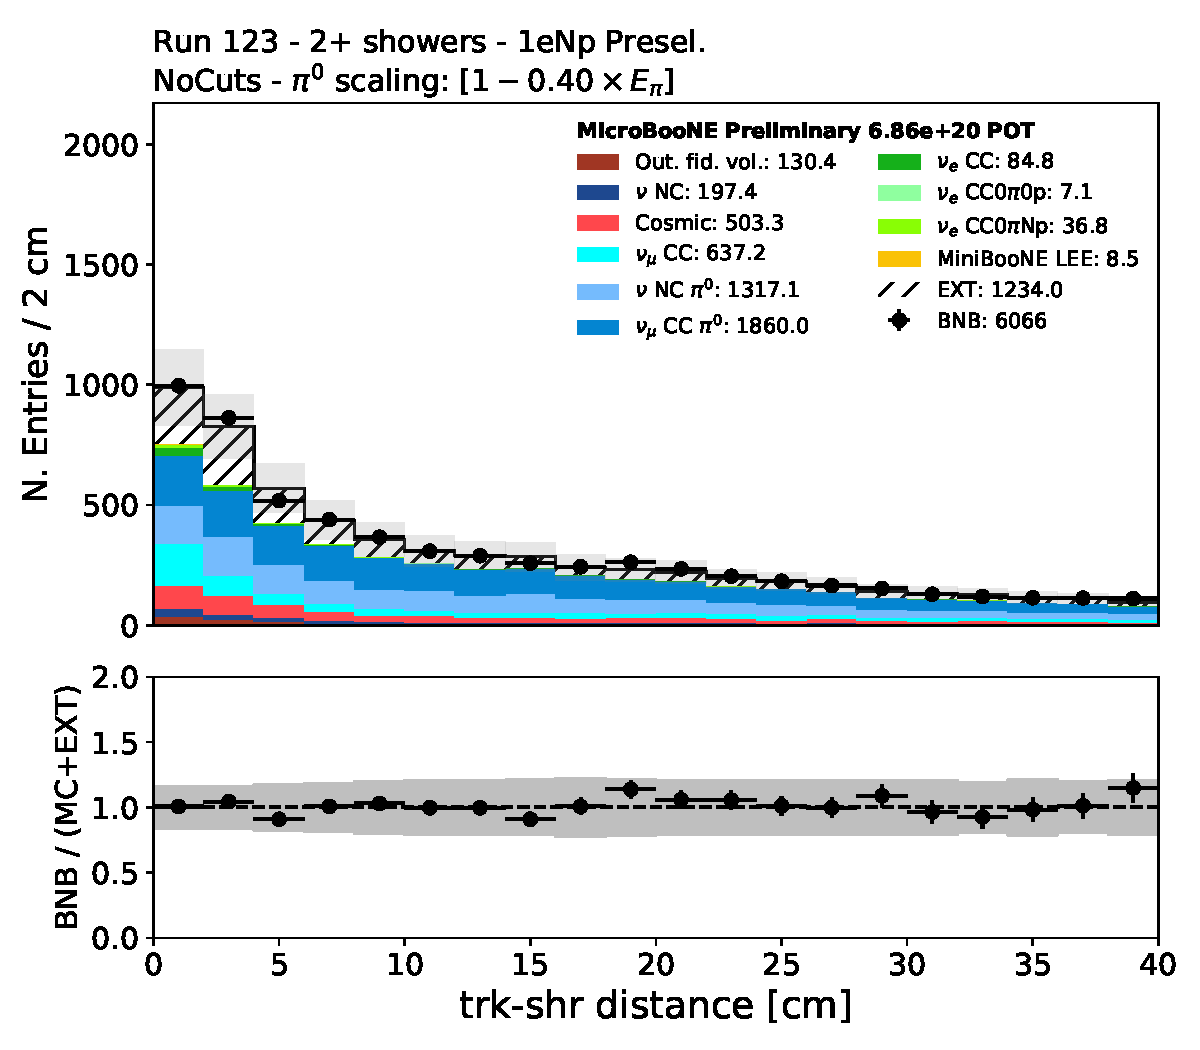
\includegraphics[width=1.0\textwidth]{Sidebands/Figures/1eNp/TwoShower/TwoPShr_NP_None_pi0e040/tksh_distance.pdf}
    \caption{tksh\_distance}
    \end{subfigure}
    \begin{subfigure}{0.3\textwidth}
    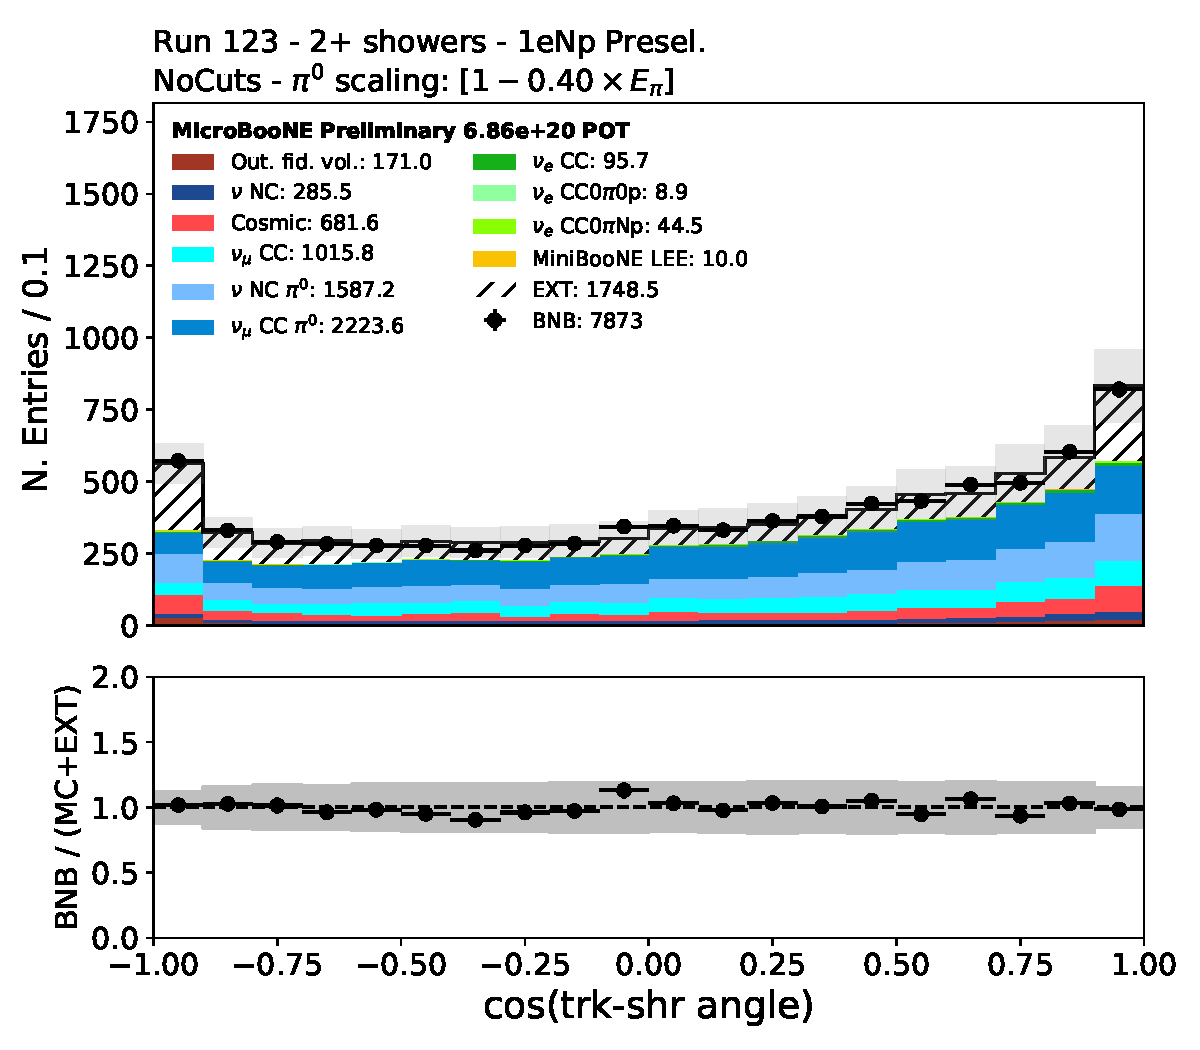
\includegraphics[width=1.0\textwidth]{Sidebands/Figures/1eNp/TwoShower/TwoPShr_NP_None_pi0e040/tksh_angle.pdf}
    \caption{tksh\_angle}
    \end{subfigure}
    \begin{subfigure}{0.3\textwidth}
    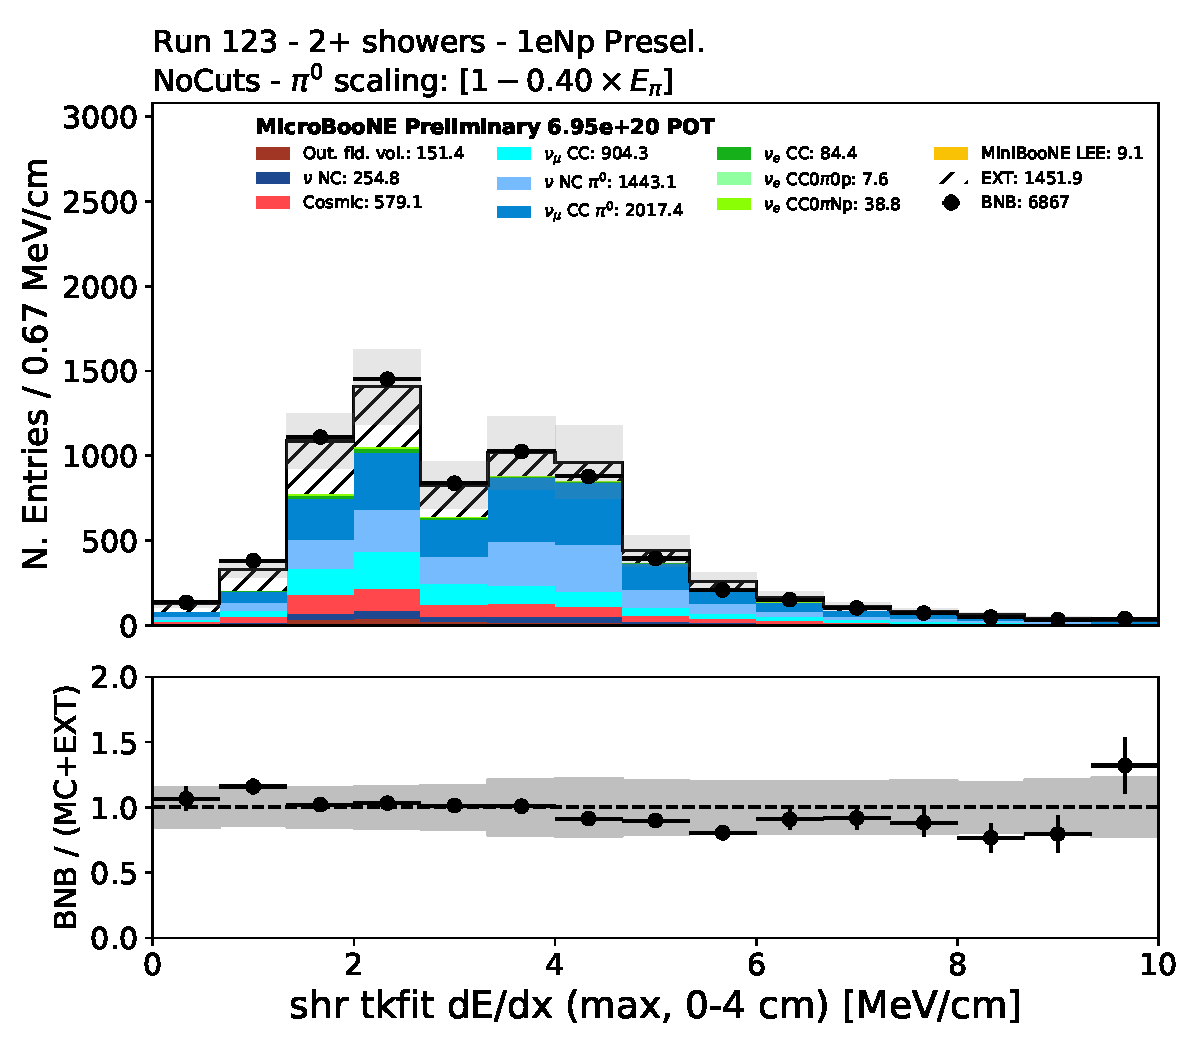
\includegraphics[width=1.0\textwidth]{Sidebands/Figures/1eNp/TwoShower/TwoPShr_NP_None_pi0e040/shr_tkfit_dedx_max.pdf}
    \caption{shr\_tkfit\_dedx\_max}
    \end{subfigure}
    \caption{} 
    \label{fig:TWOP_1eNp_1}
\end{figure}

\begin{figure}[H]
    \centering
    \begin{subfigure}{0.3\textwidth}
    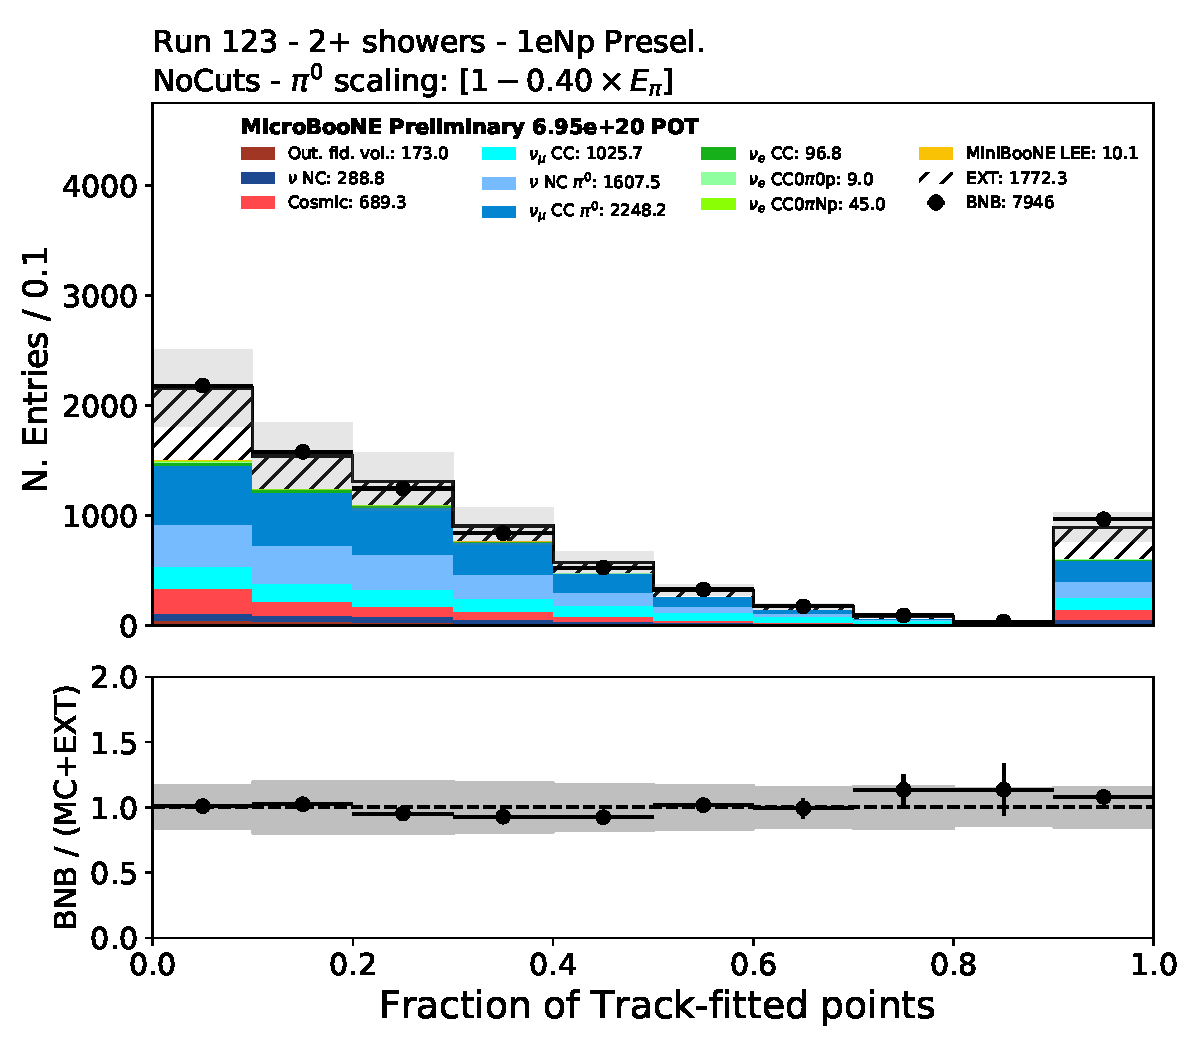
\includegraphics[width=1.0\textwidth]{Sidebands/Figures/1eNp/TwoShower/TwoPShr_NP_None_pi0e040/trkfit.pdf}
    \caption{trkfit}
    \end{subfigure}
    \begin{subfigure}{0.3\textwidth}
    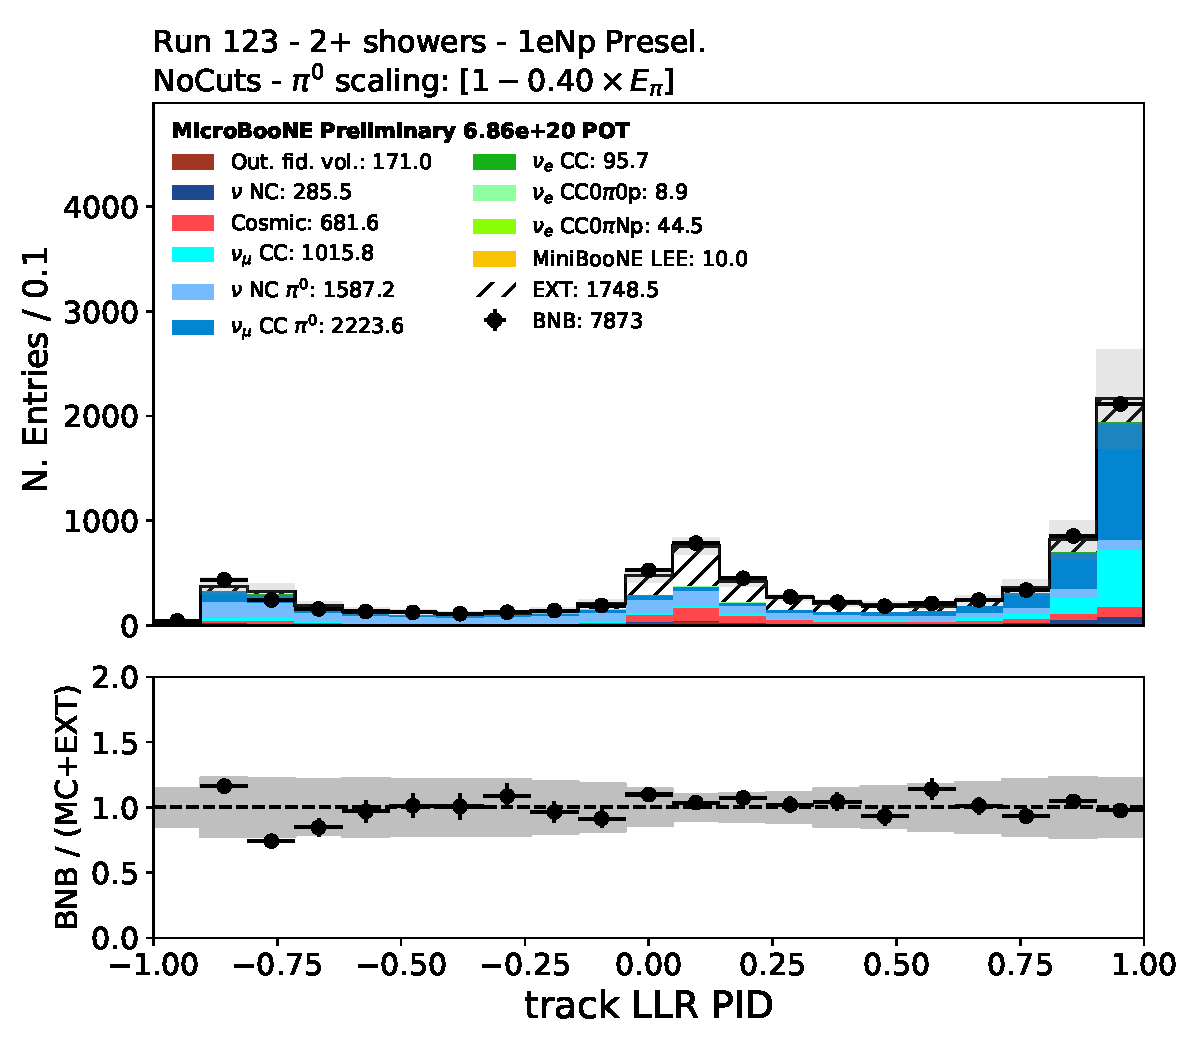
\includegraphics[width=1.0\textwidth]{Sidebands/Figures/1eNp/TwoShower/TwoPShr_NP_None_pi0e040/trkpid.pdf}
    \caption{trkpid}
    \end{subfigure}
    \begin{subfigure}{0.3\textwidth}
    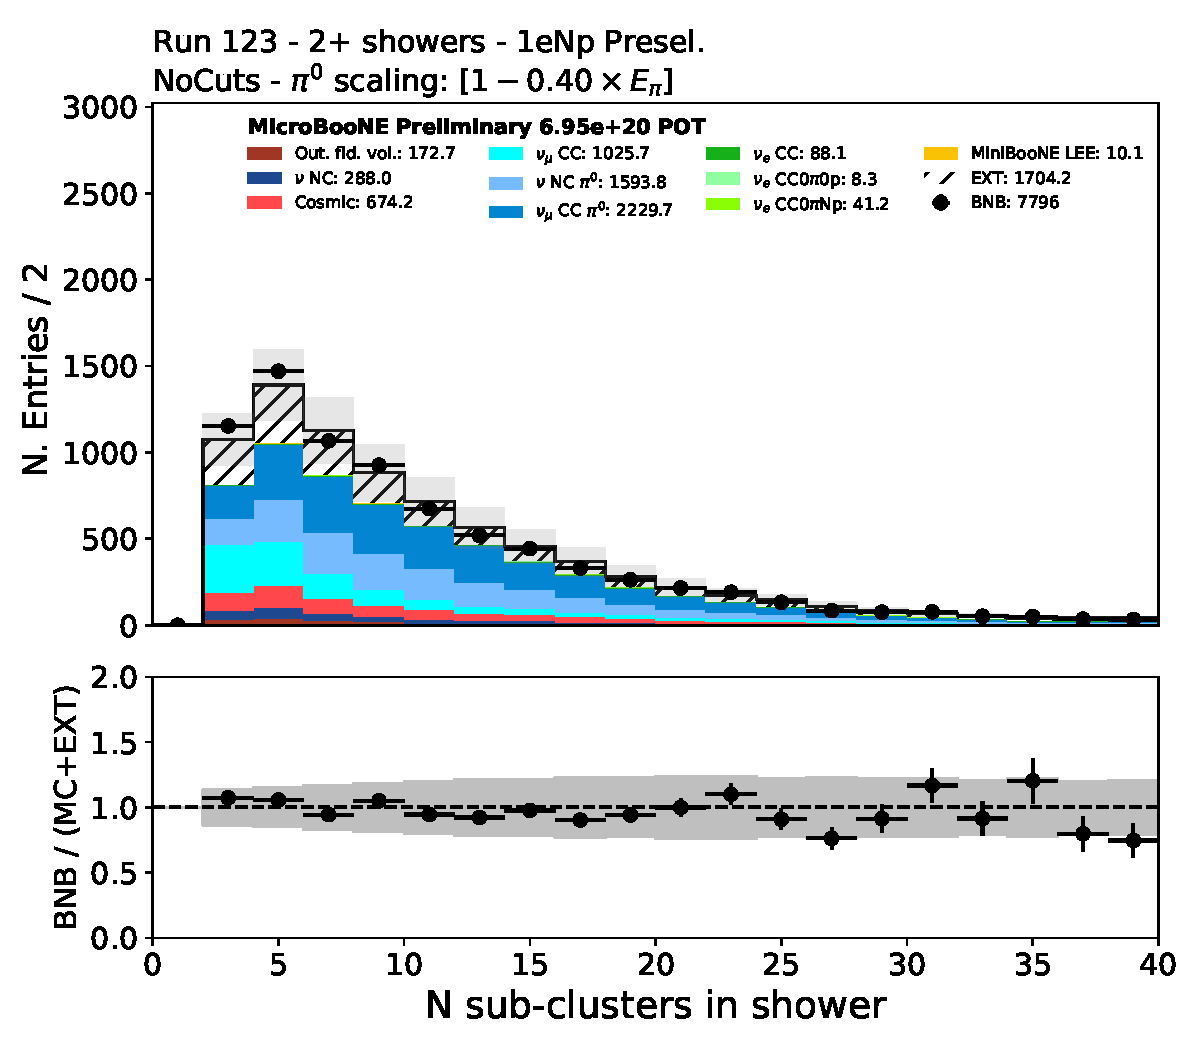
\includegraphics[width=1.0\textwidth]{Sidebands/Figures/1eNp/TwoShower/TwoPShr_NP_None_pi0e040/subcluster.pdf}
    \caption{subcluster}
    \end{subfigure}
    \caption{} 
    \label{fig:TWOP_1eNp_2}
\end{figure}

\begin{figure}[H]
    \centering
    \begin{subfigure}{0.3\textwidth}
    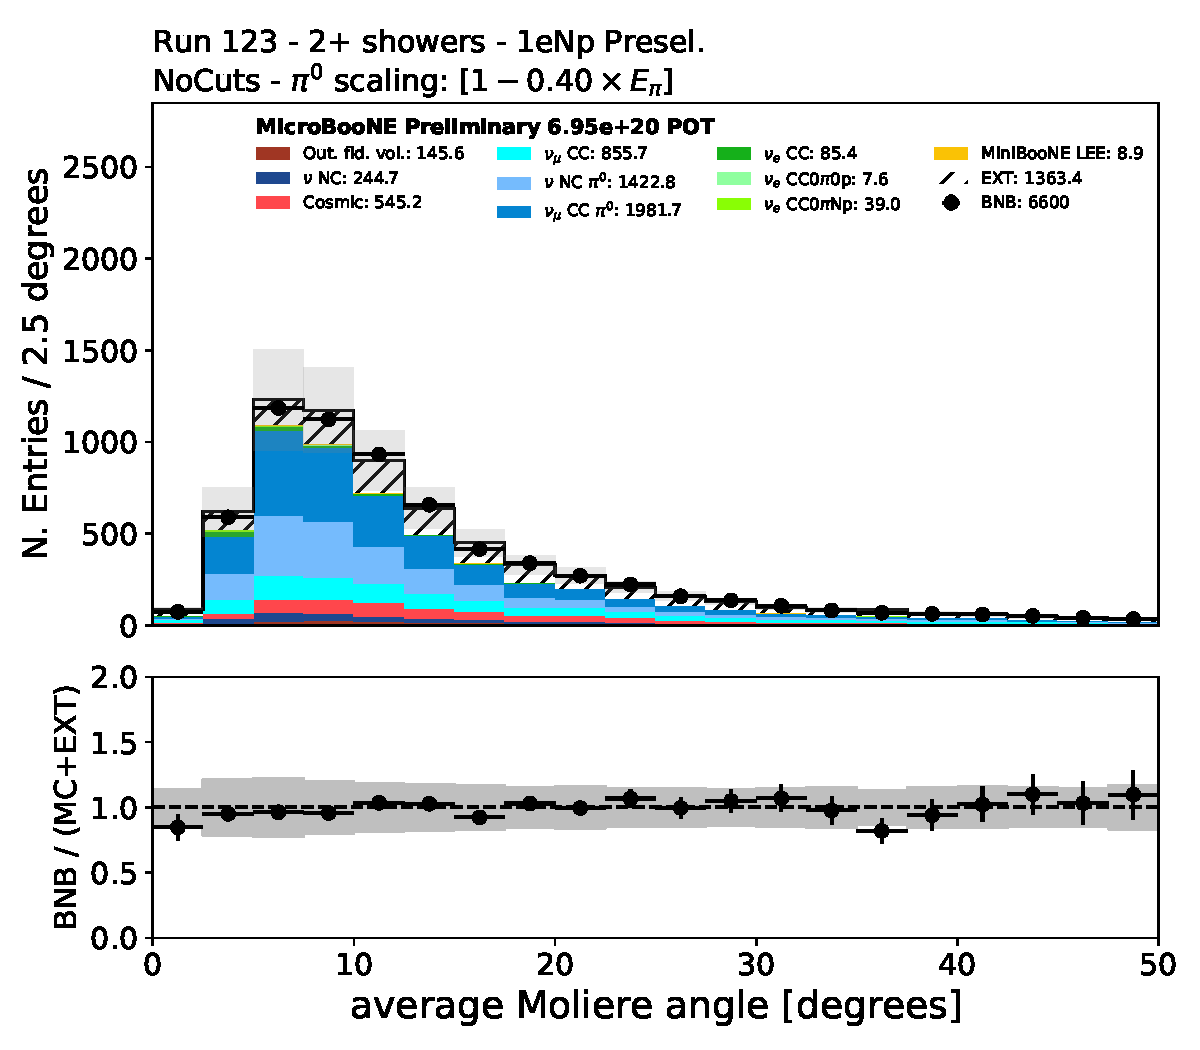
\includegraphics[width=1.0\textwidth]{Sidebands/Figures/1eNp/TwoShower/TwoPShr_NP_None_pi0e040/shrmoliereavg.pdf}
    \caption{shrmoliereavg}
    \end{subfigure}
    \begin{subfigure}{0.3\textwidth}
    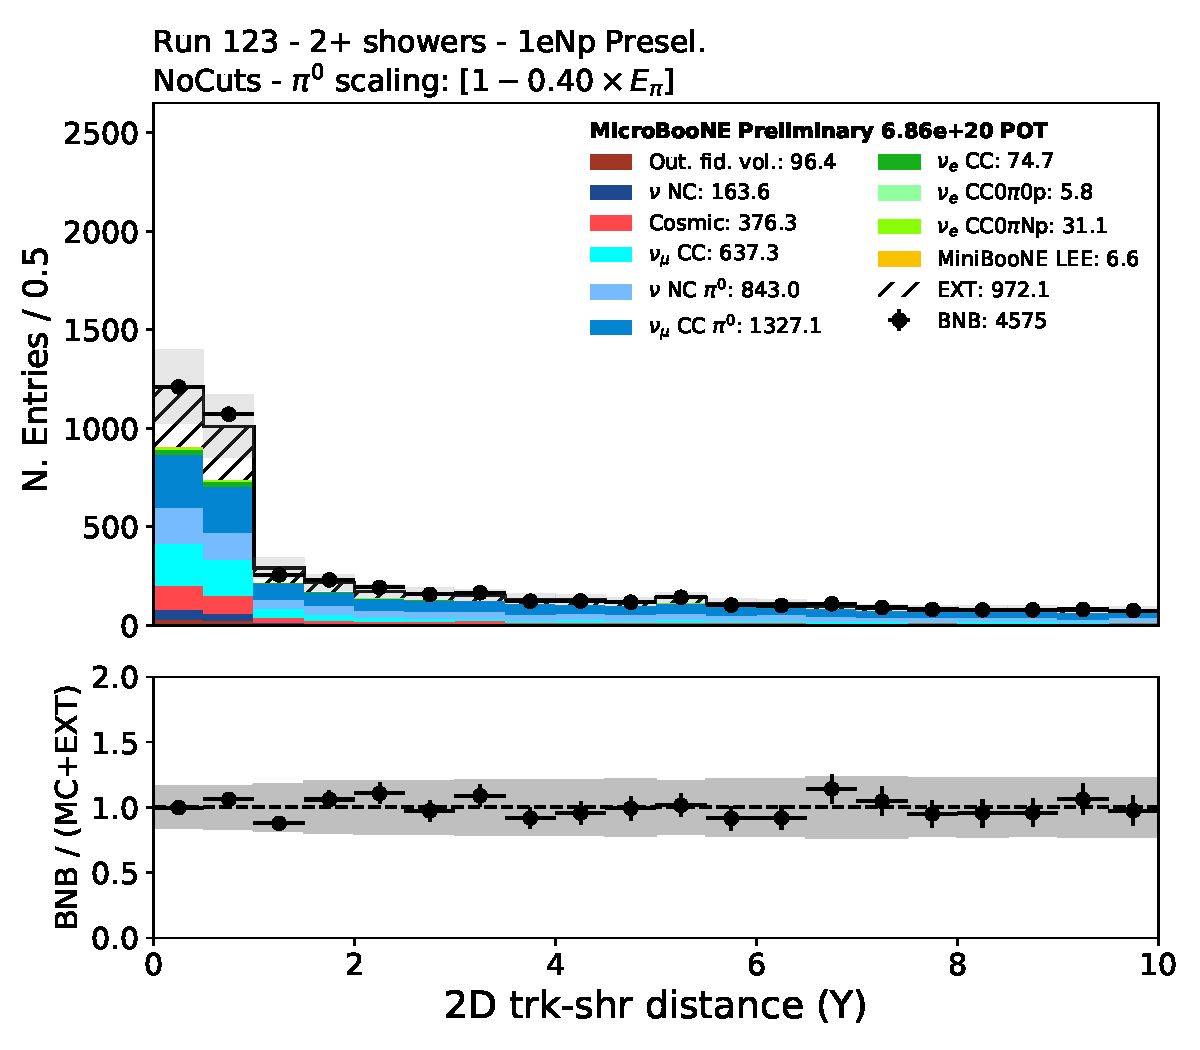
\includegraphics[width=1.0\textwidth]{Sidebands/Figures/1eNp/TwoShower/TwoPShr_NP_None_pi0e040/trkshrhitdist2.pdf}
    \caption{tkshrhitdist2}
    \end{subfigure}
    \begin{subfigure}{0.3\textwidth}
    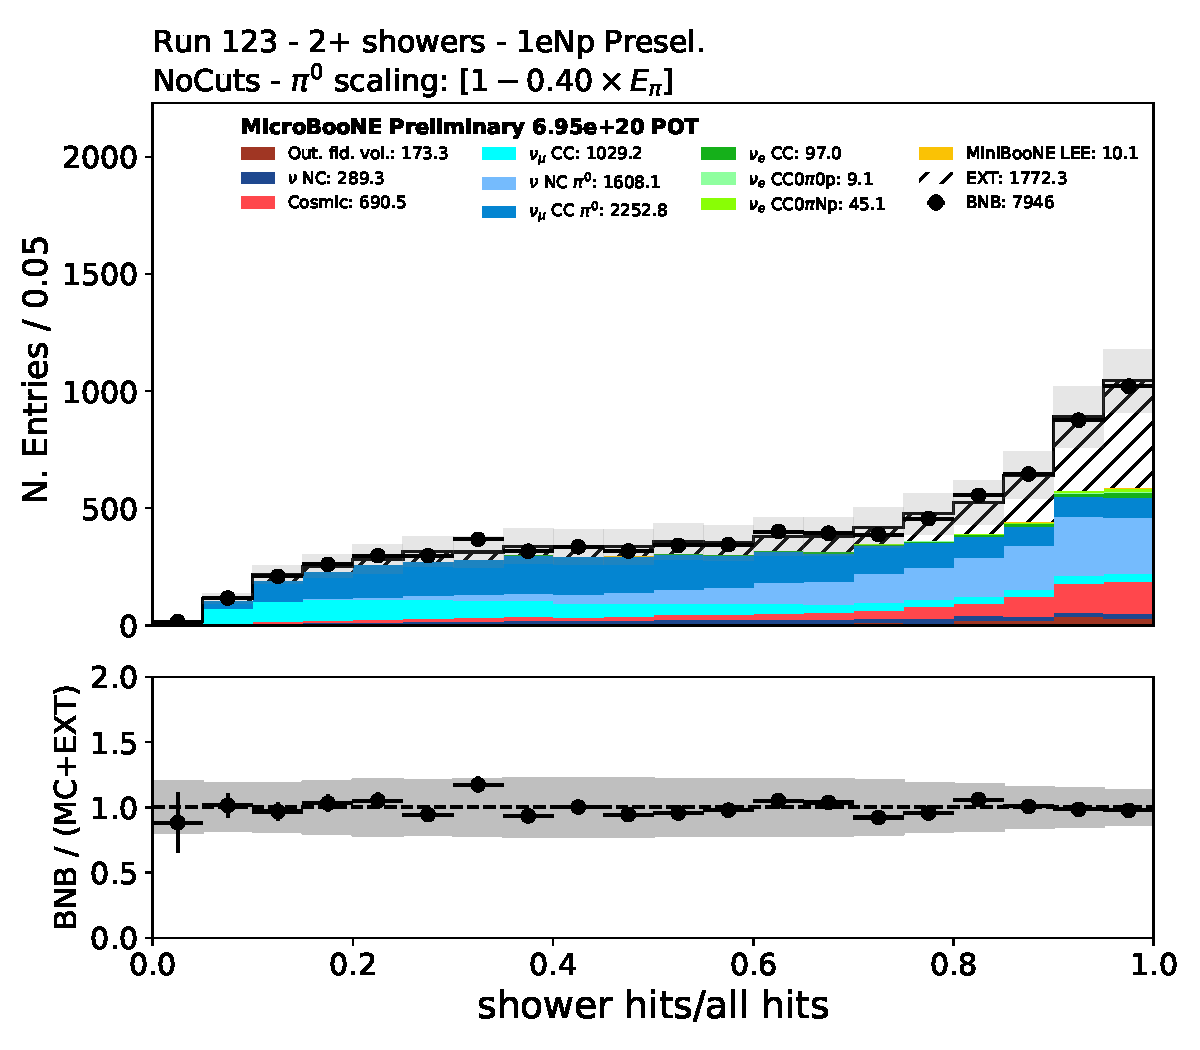
\includegraphics[width=1.0\textwidth]{Sidebands/Figures/1eNp/TwoShower/TwoPShr_NP_None_pi0e040/hits_ratio.pdf}
    \caption{hits\_ratio}
    \end{subfigure}
    \caption{} 
    \label{fig:TWOP_1eNp_3}
\end{figure}

\begin{figure}[H]
    \centering
    \begin{subfigure}{0.3\textwidth}
    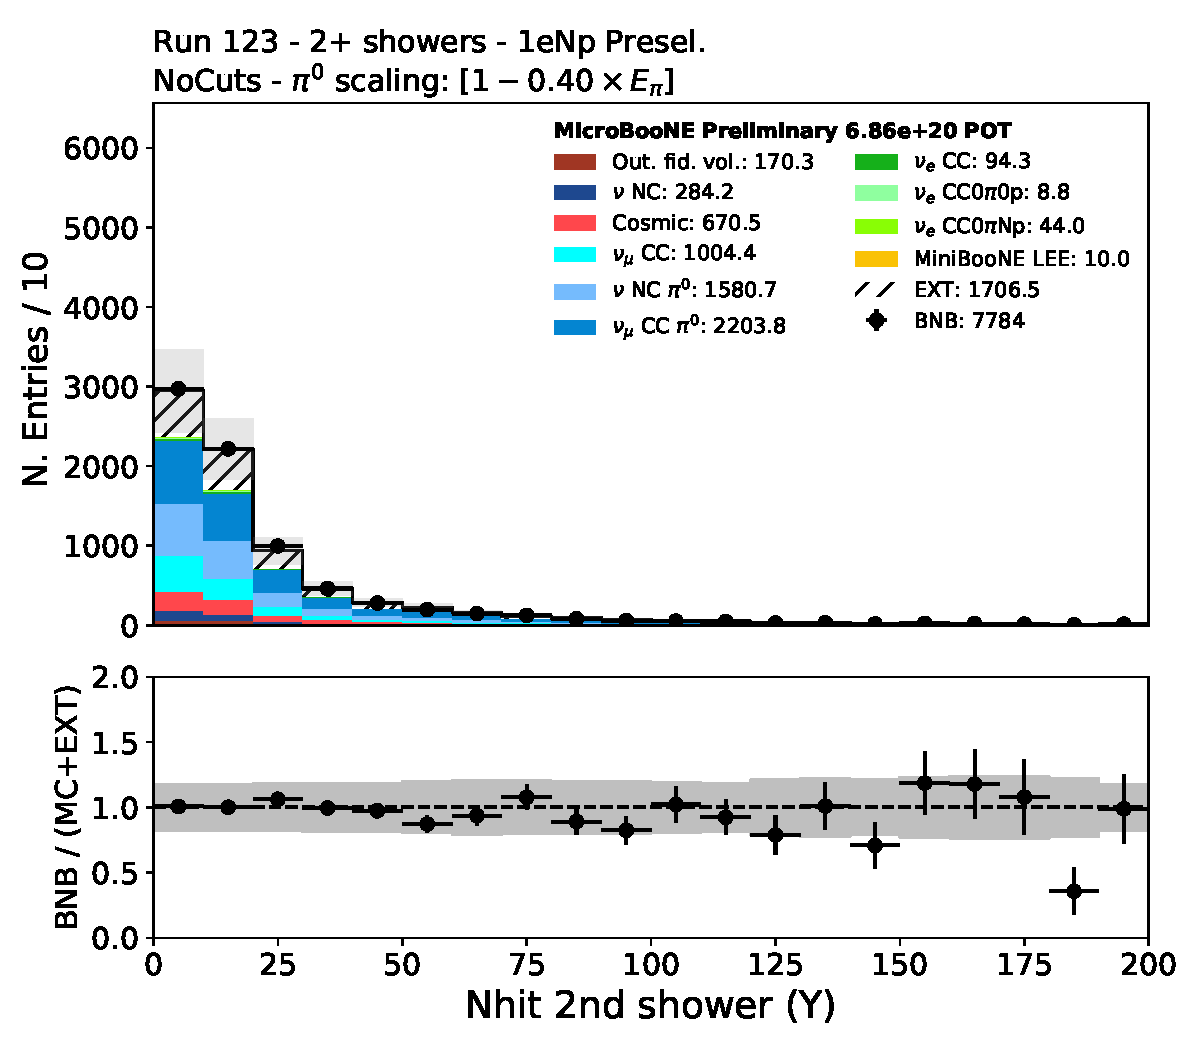
\includegraphics[width=1.0\textwidth]{Sidebands/Figures/1eNp/TwoShower/TwoPShr_NP_None_pi0e040/secondshower_Y_nhit.pdf}
    \caption{secondshower\_Y\_nhit}
    \end{subfigure}
    \begin{subfigure}{0.3\textwidth}
    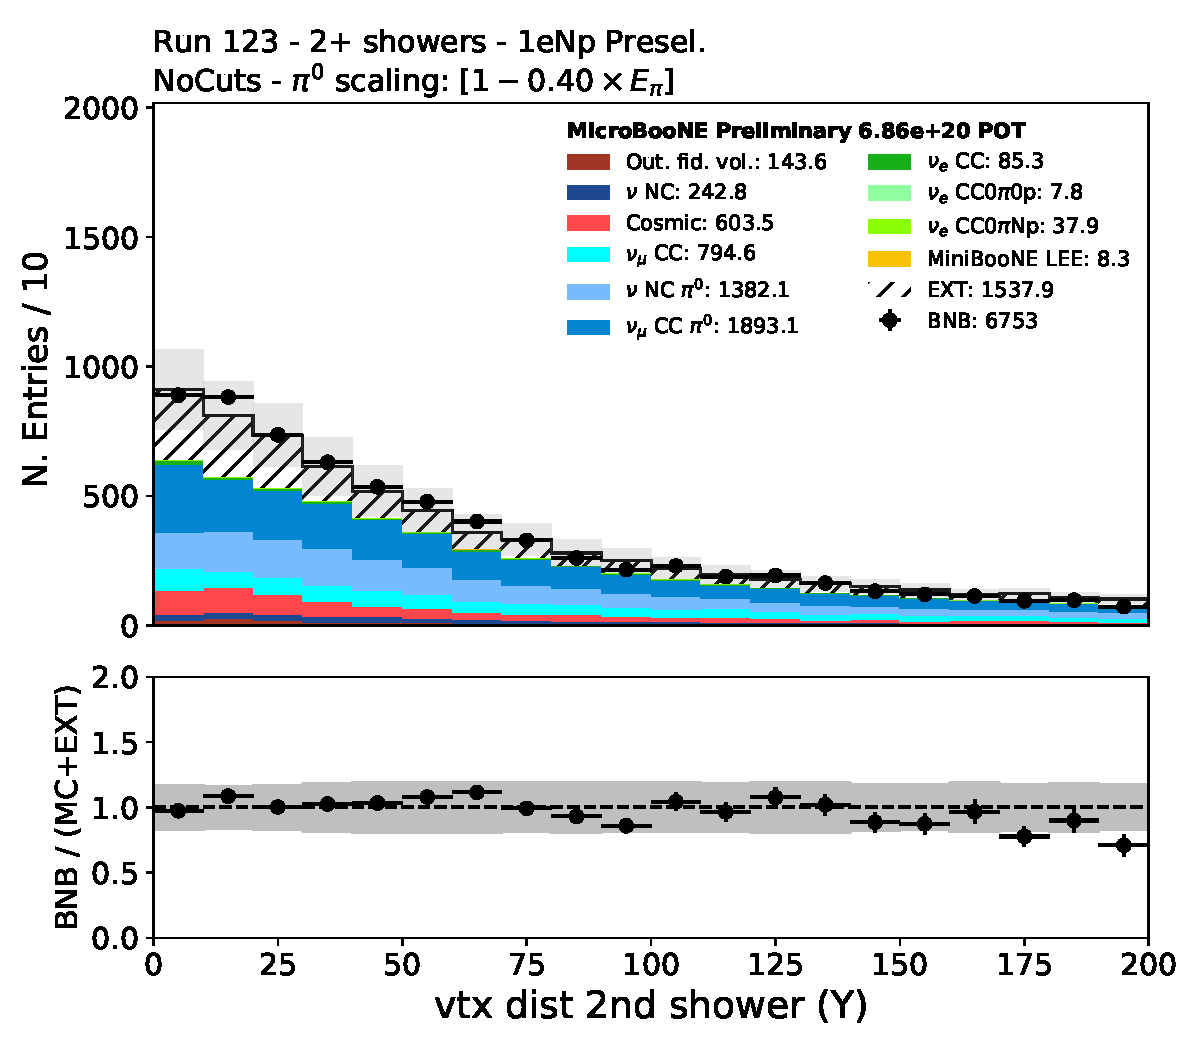
\includegraphics[width=1.0\textwidth]{Sidebands/Figures/1eNp/TwoShower/TwoPShr_NP_None_pi0e040/secondshower_Y_vtxdist.pdf}
    \caption{secondshower\_Y\_vtxdist}
    \end{subfigure}
    \begin{subfigure}{0.3\textwidth}
    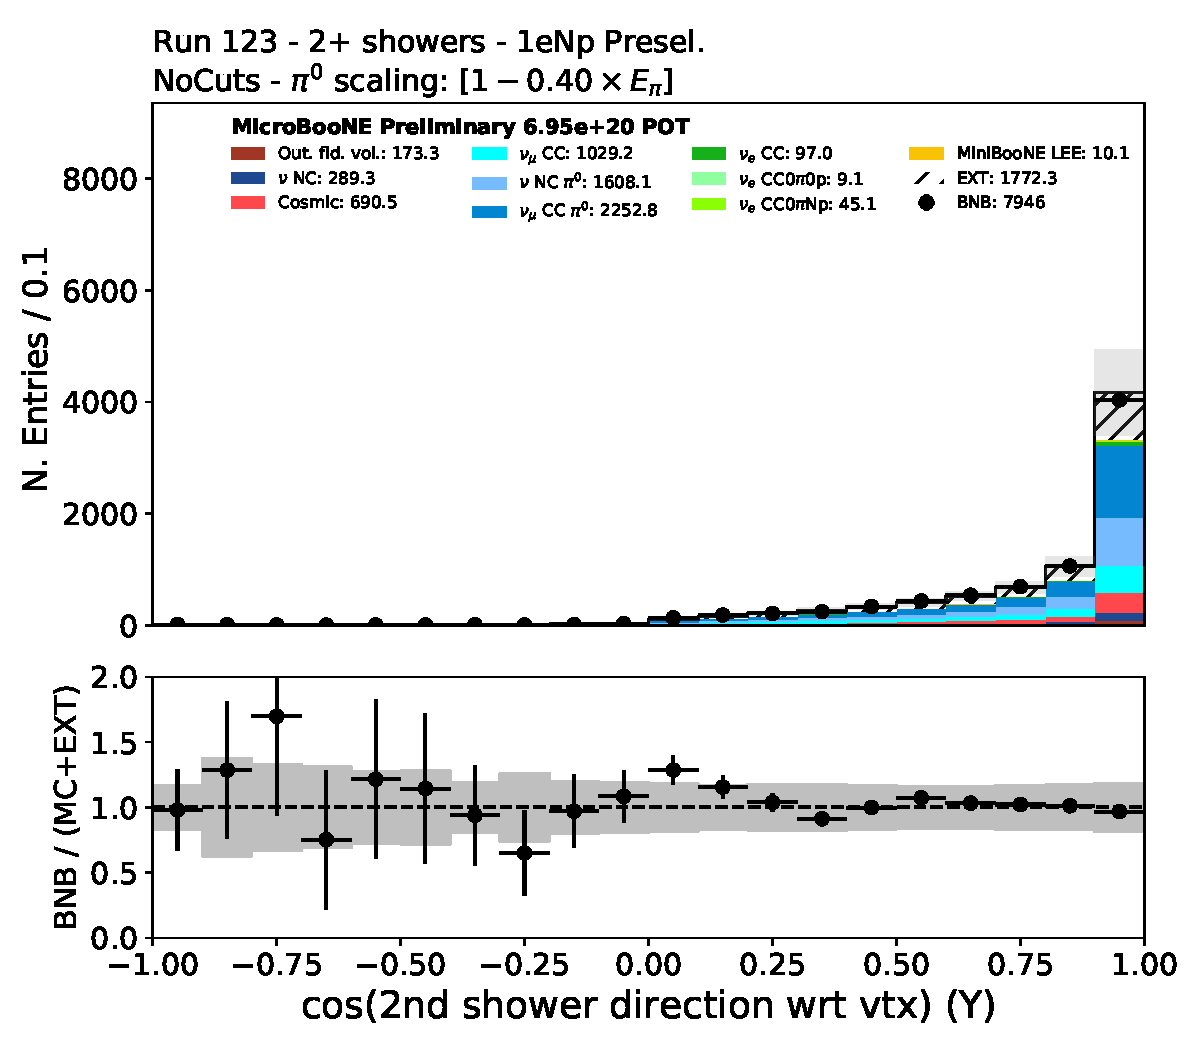
\includegraphics[width=1.0\textwidth]{Sidebands/Figures/1eNp/TwoShower/TwoPShr_NP_None_pi0e040/secondshower_Y_dot.pdf}
    \caption{secondshower\_Y\_dot}
    \end{subfigure}
    \caption{} 
    \label{fig:TWOP_1eNp_4}
\end{figure}

\begin{figure}[H]
    \centering
    \begin{subfigure}{0.3\textwidth}
    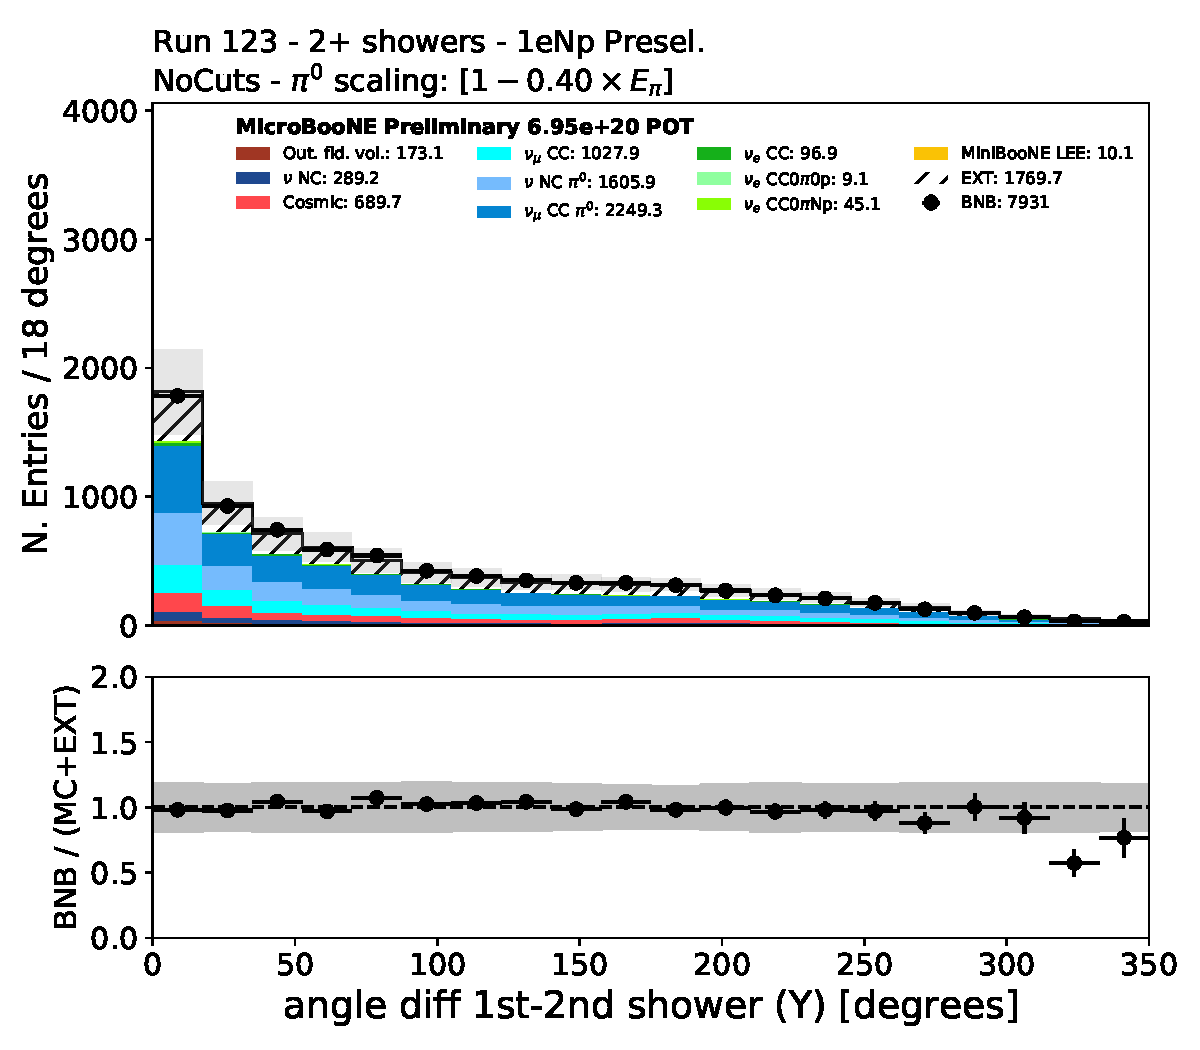
\includegraphics[width=1.0\textwidth]{Sidebands/Figures/1eNp/TwoShower/TwoPShr_NP_None_pi0e040/anglediff_Y.pdf}
    \caption{anglediff\_Y}
    \end{subfigure}
    \begin{subfigure}{0.3\textwidth}
    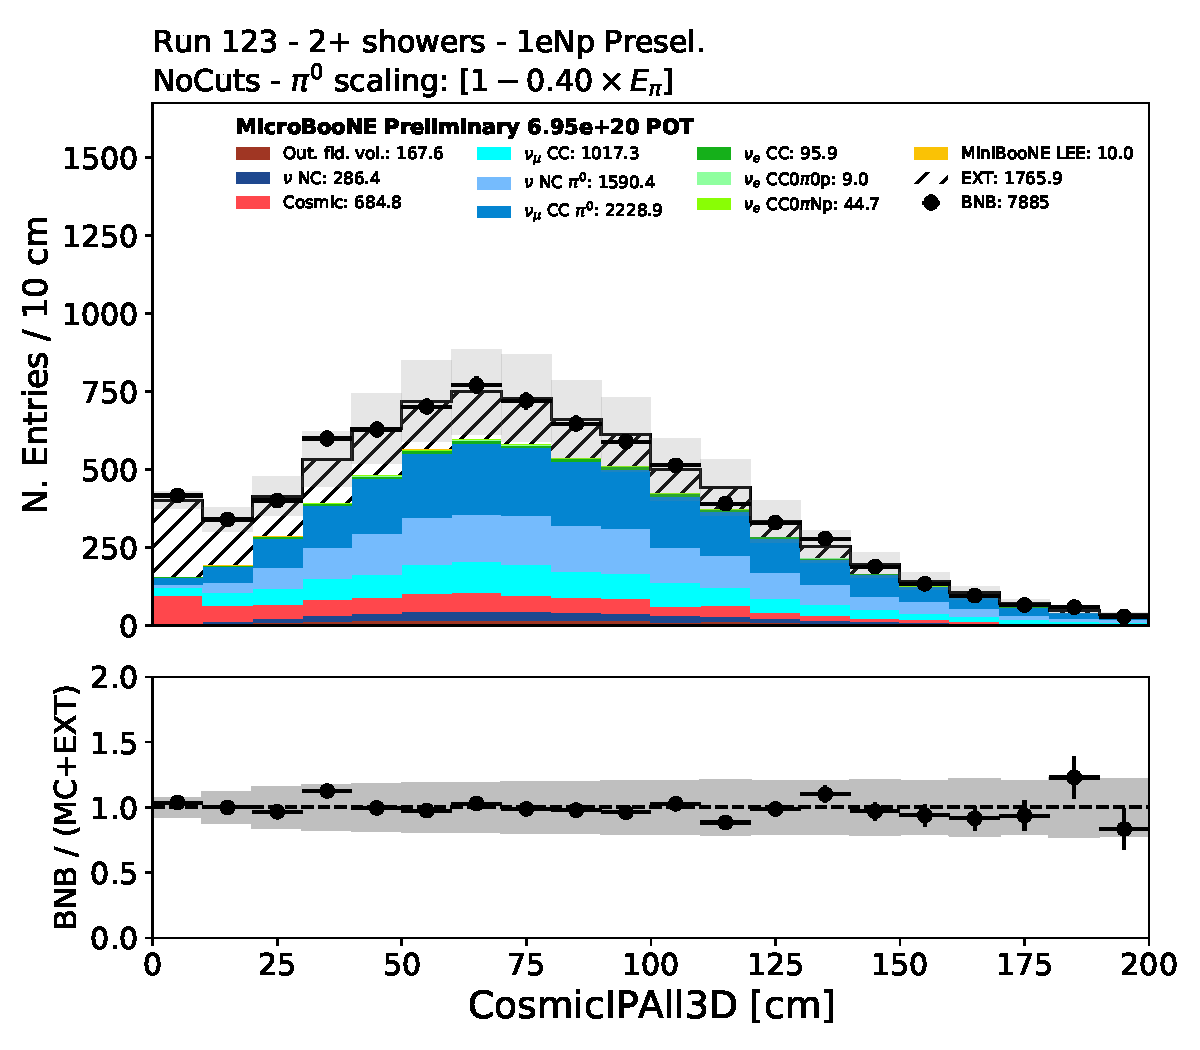
\includegraphics[width=1.0\textwidth]{Sidebands/Figures/1eNp/TwoShower/TwoPShr_NP_None_pi0e040/CosmicIPAll3D.pdf}
    \caption{CosmicIPAll3D}
    \end{subfigure}
    \begin{subfigure}{0.3\textwidth}
    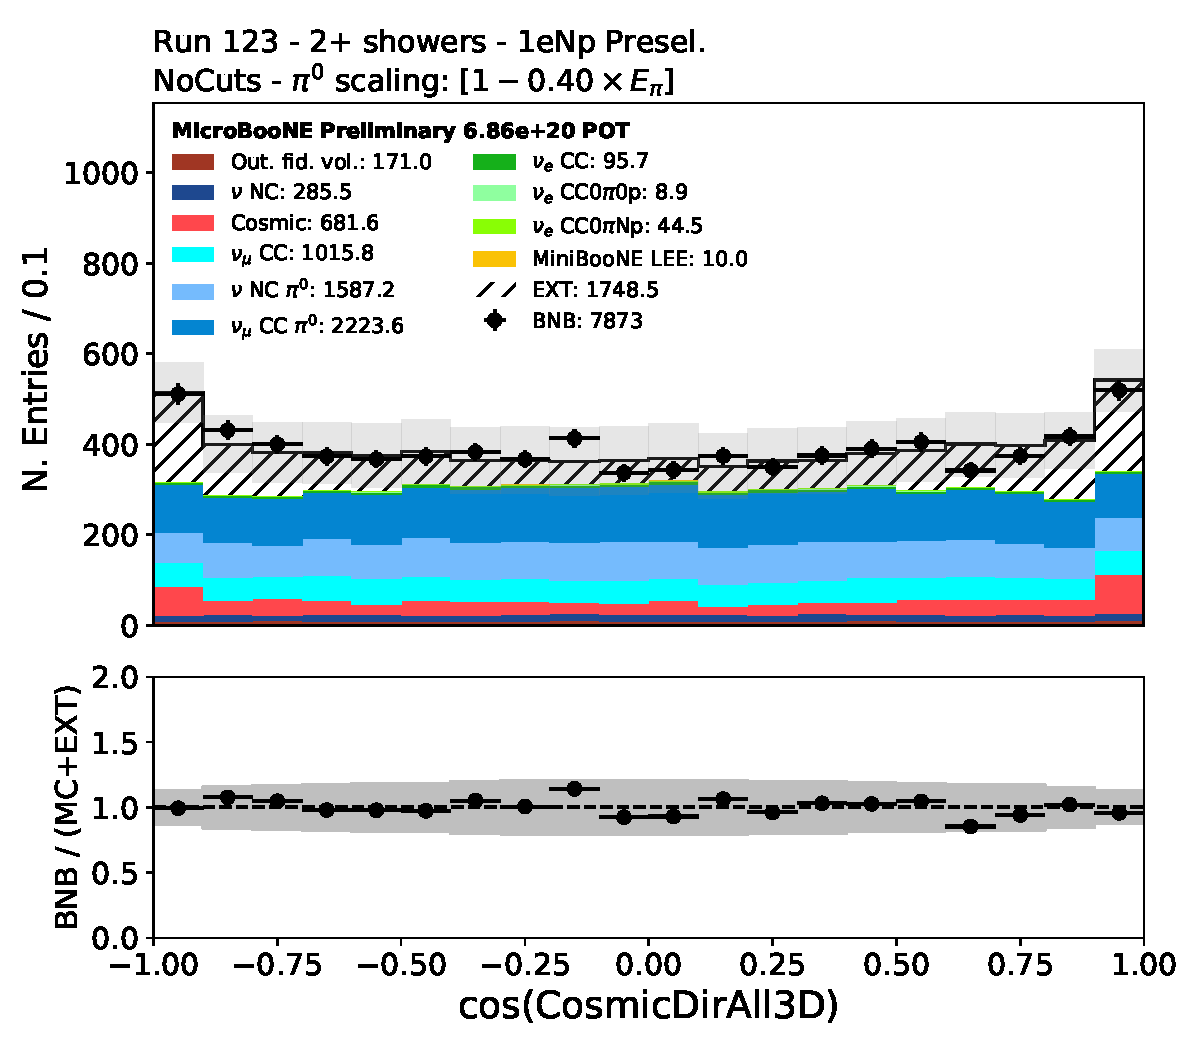
\includegraphics[width=1.0\textwidth]{Sidebands/Figures/1eNp/TwoShower/TwoPShr_NP_None_pi0e040/CosmicDirAll3D.pdf}
    \caption{CosmidDirAll3D}
    \end{subfigure}
    \caption{} 
    \label{fig:TWOP_1eNp_5}
\end{figure}
Figure~\ref{fig:sb:1eNp:twopshr:BDT} shows the \npsel BDT response in the two shower sideband.

\begin{figure}[H]
    \begin{center}
    \begin{subfigure}{0.45\textwidth}
    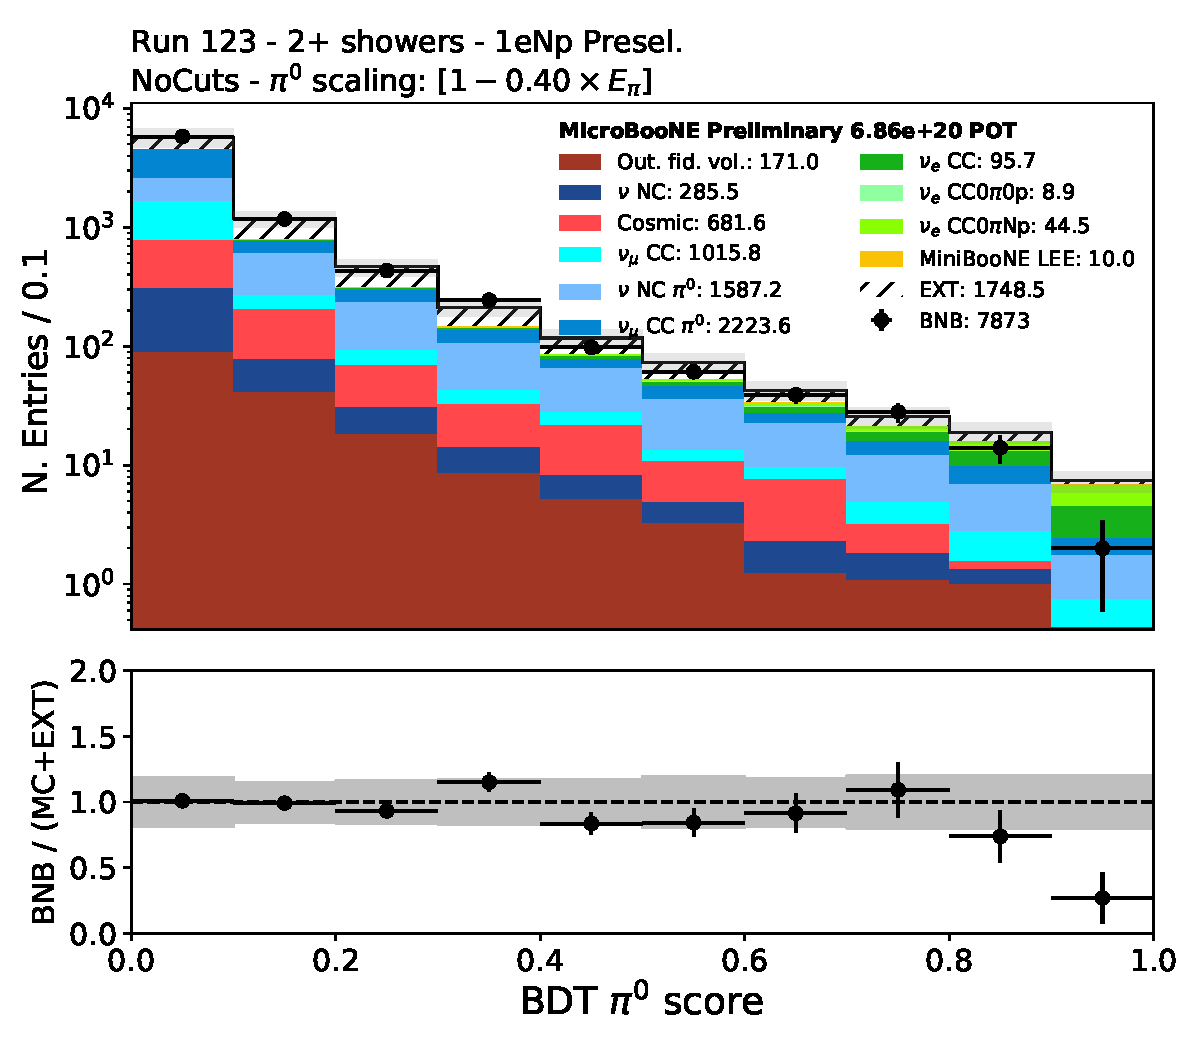
\includegraphics[width=1.00\textwidth]{Sidebands/Figures/1eNp/TwoShower/TwoPShr_NP_None_pi0e040/pi0_score_log.pdf}
    \caption{\npsel $\pi^0$ BDT response}
    \end{subfigure}
    \begin{subfigure}{0.45\textwidth}
    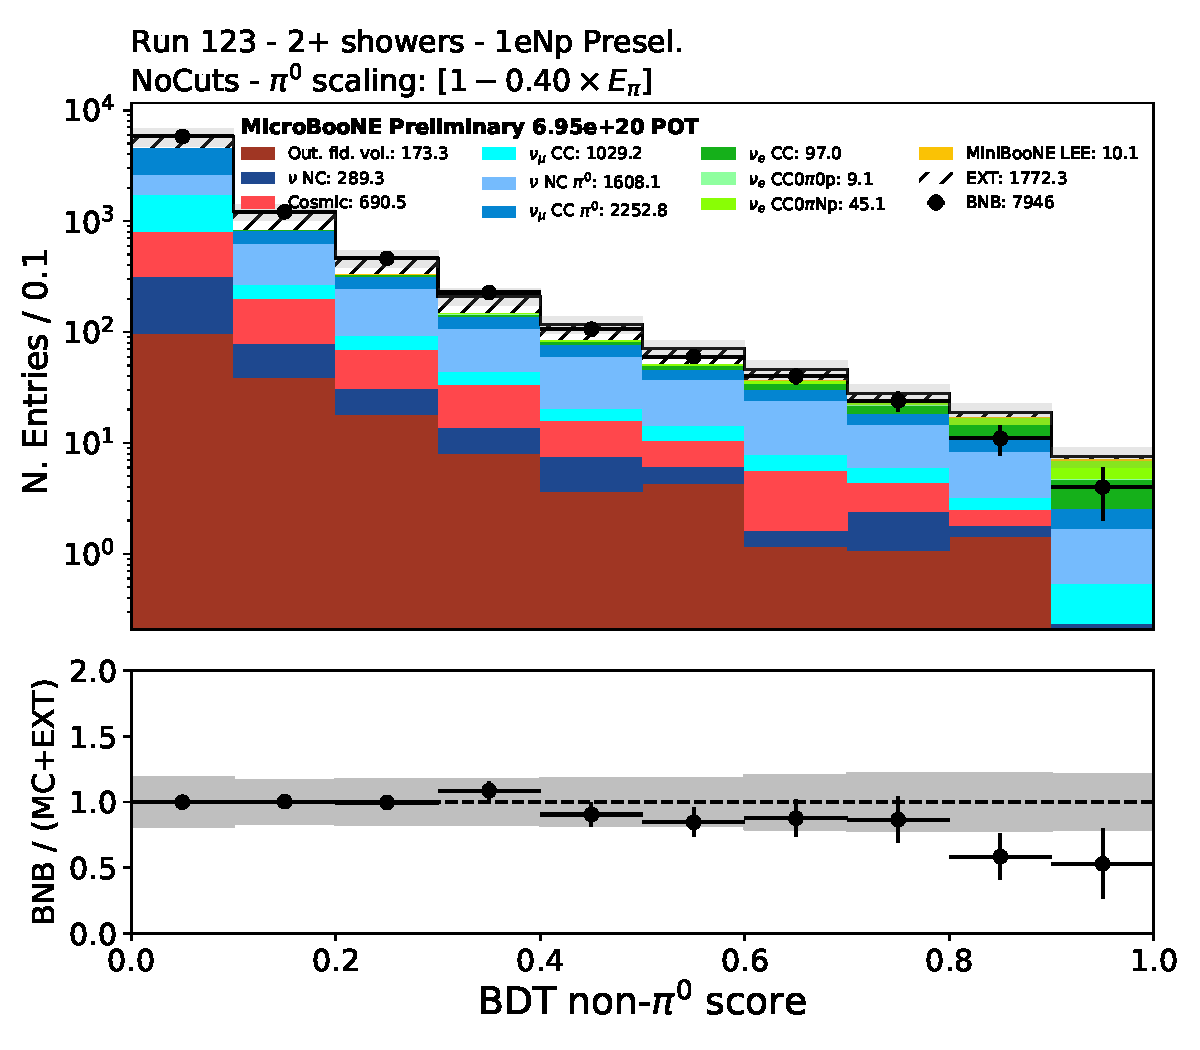
\includegraphics[width=1.00\textwidth]{Sidebands/Figures/1eNp/TwoShower/TwoPShr_NP_None_pi0e040/nonpi0_score_log.pdf}
    \caption{\npsel non-$\pi^0$ BDT response}
    \end{subfigure} \\
    \caption{\label{fig:sb:1eNp:twopshr:BDT} BDT response in the 2+ shower sideband.}
    \end{center}
\end{figure}

The Loose selection is also a stage where we can check the modeling of the most important selection variables in the analysis. These are shown in Fig.~\ref{fig:sb:1eNp:twopshr:loose:vars1}-\ref{fig:sb:1eNp:twopshr:loose:vars2}, and demonstrate good agreement with the prediction. The BDT responses are shown in Fig.~\ref{fig:sb:1eNp:twopshr:loose:bdt}.

\begin{figure}[H]
    \begin{center}
    \begin{subfigure}{0.45\textwidth}
    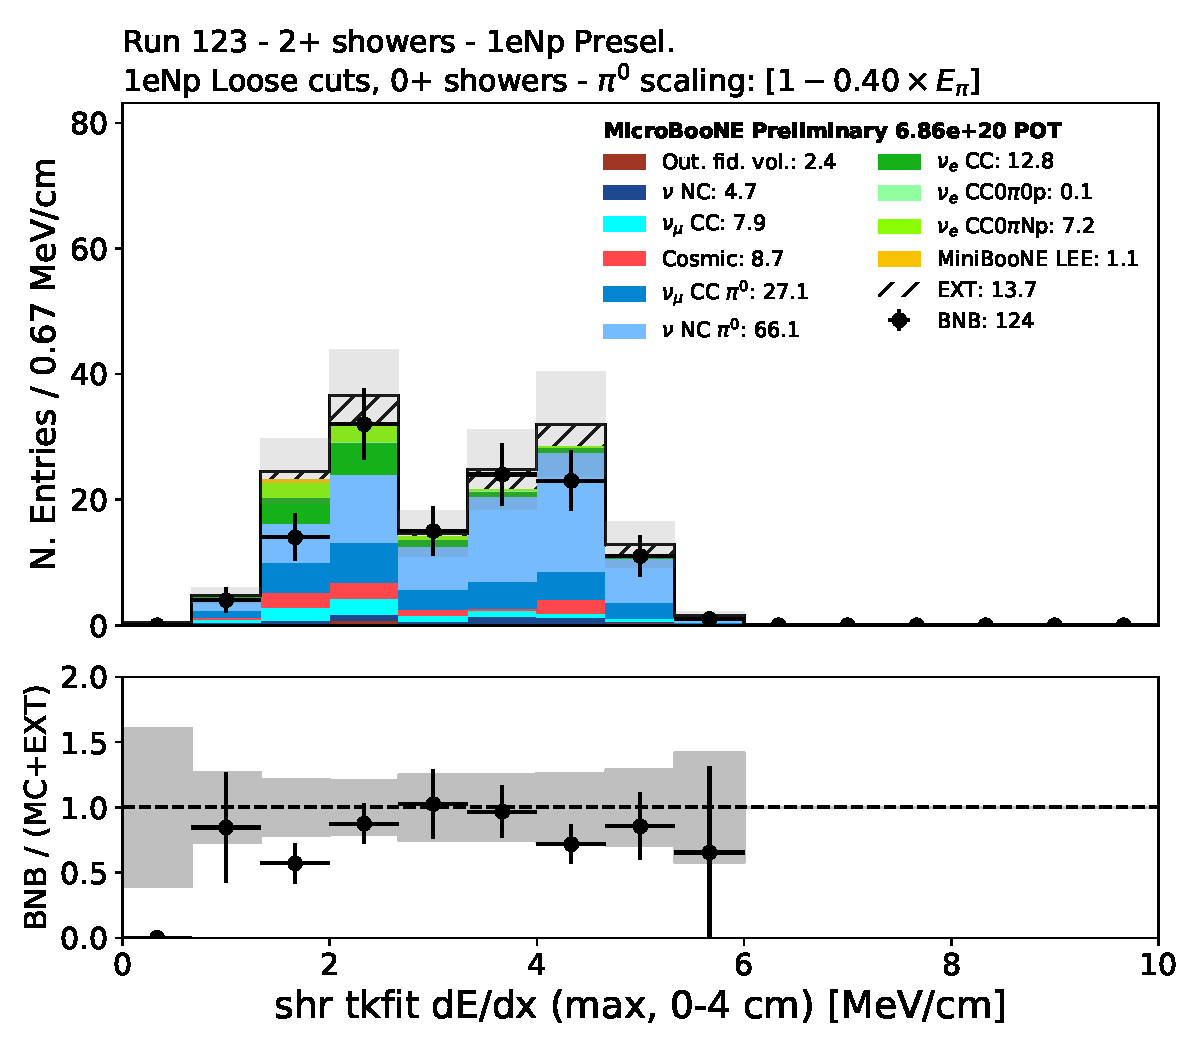
\includegraphics[width=1.00\textwidth]{Sidebands/Figures/1eNp/TwoShower/TwoPShr_NP_NPLAllShr_pi0e040/shr_tkfit_dedx_max.pdf}
    %\caption{}
    \end{subfigure}
    \begin{subfigure}{0.45\textwidth}
    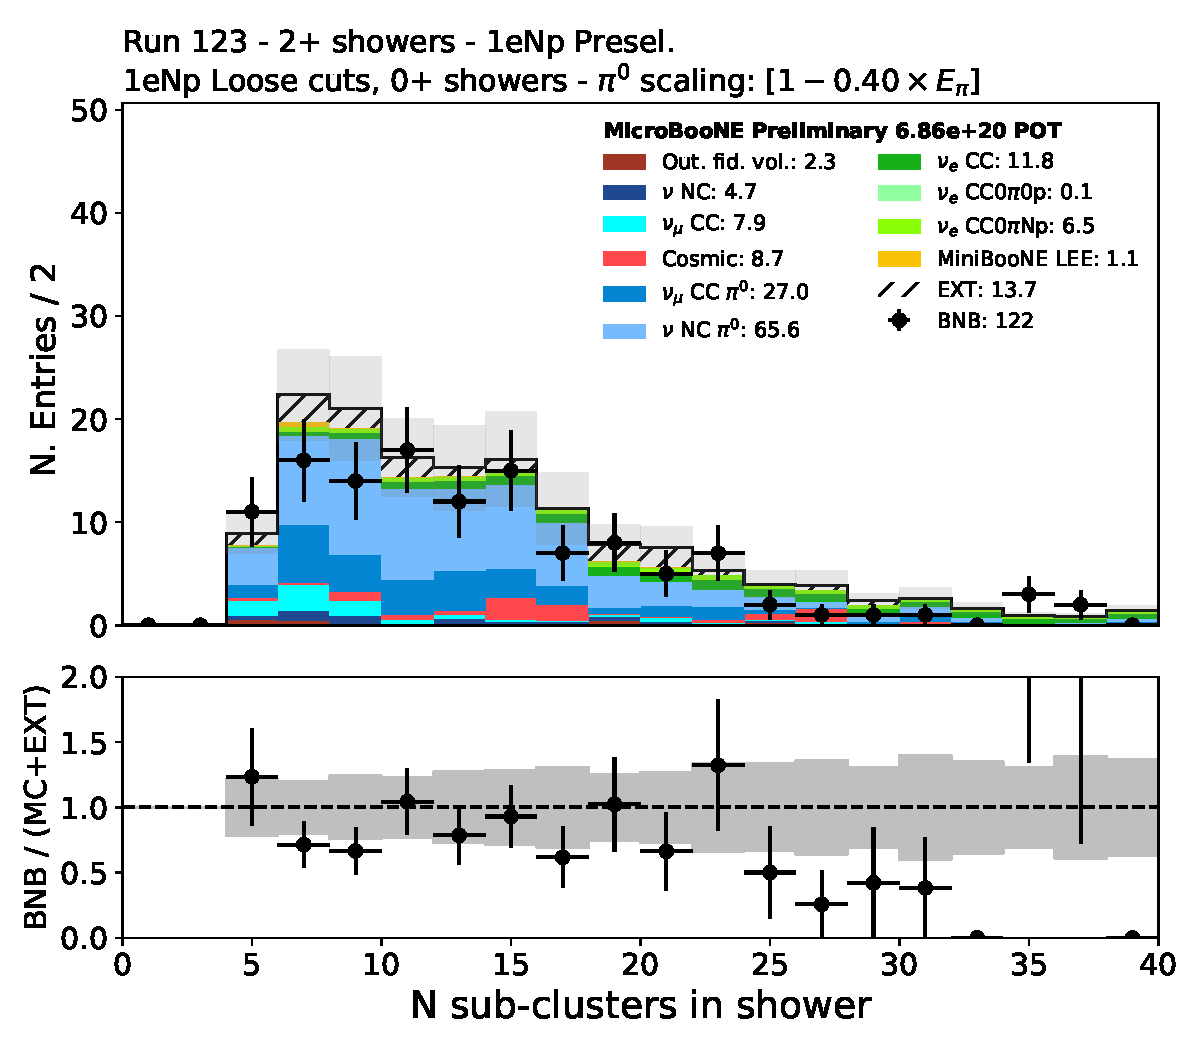
\includegraphics[width=1.00\textwidth]{Sidebands/Figures/1eNp/TwoShower/TwoPShr_NP_NPLAllShr_pi0e040/subcluster.pdf}
    %\caption{}
    \end{subfigure} \\
    \begin{subfigure}{0.45\textwidth}
    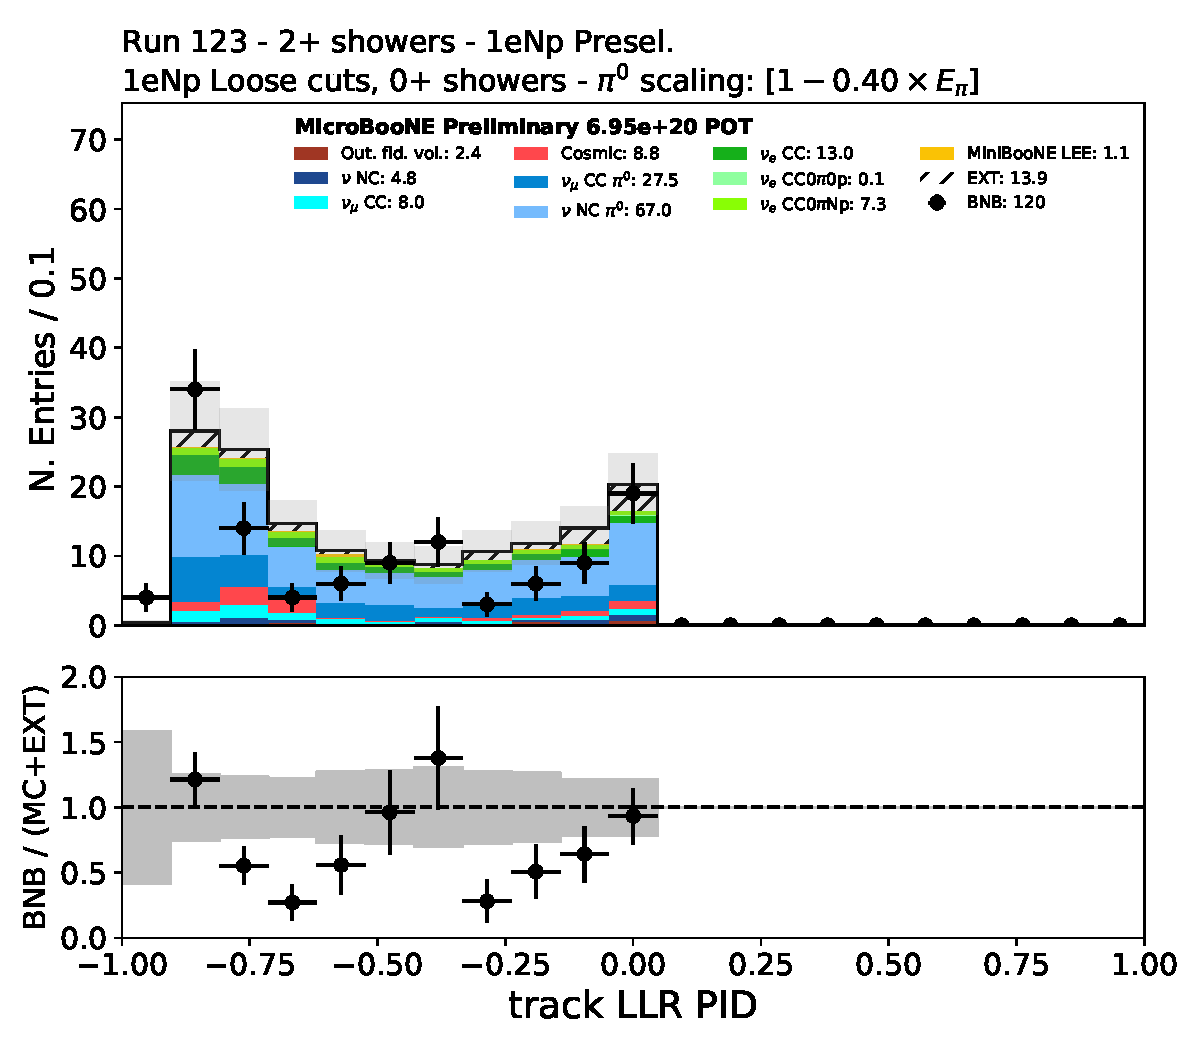
\includegraphics[width=1.00\textwidth]{Sidebands/Figures/1eNp/TwoShower/TwoPShr_NP_NPLAllShr_pi0e040/trkpid.pdf}
    %\caption{}
    \end{subfigure}
    \begin{subfigure}{0.45\textwidth}
    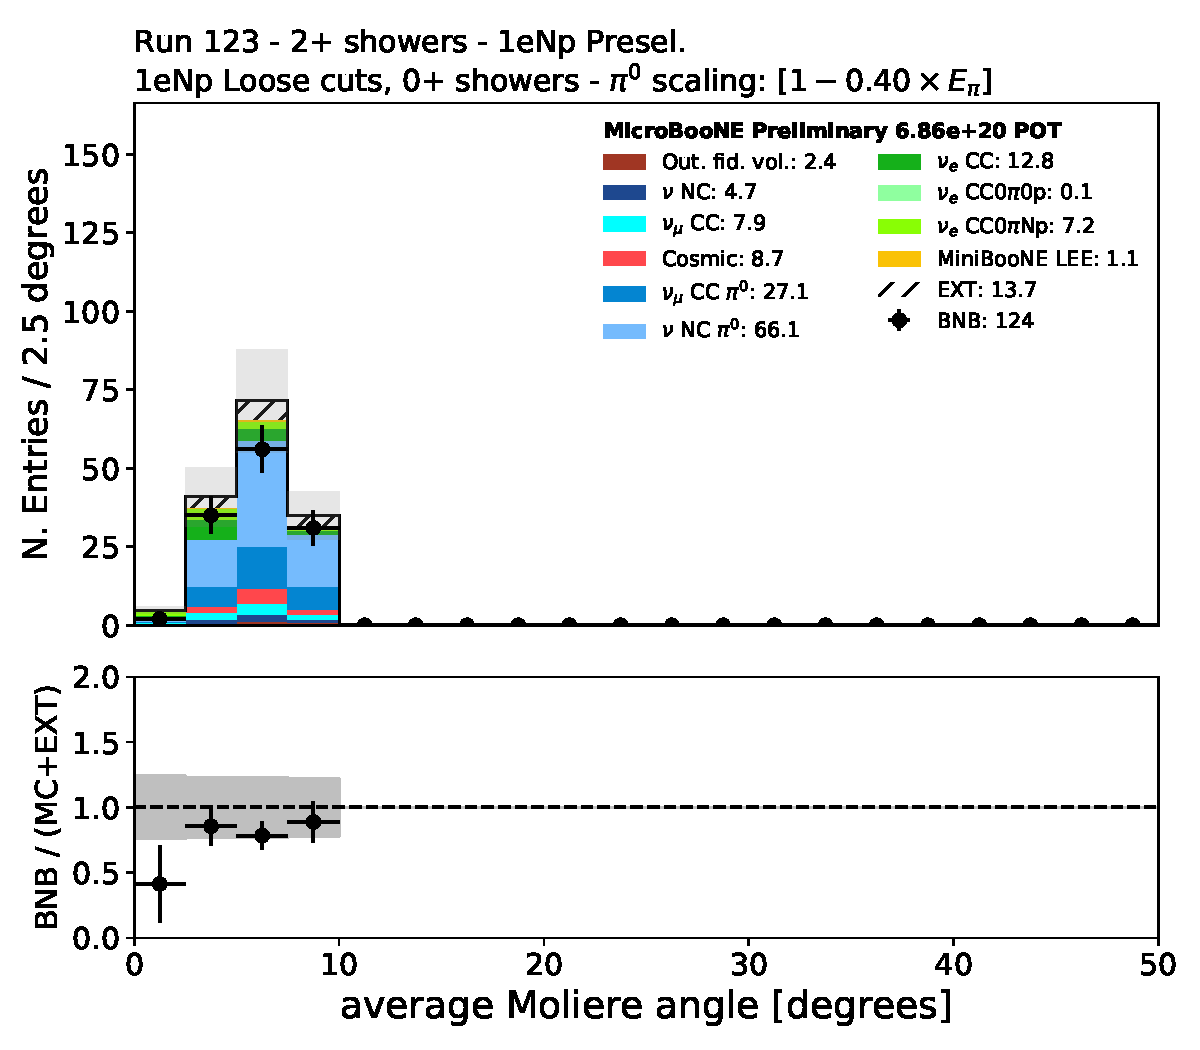
\includegraphics[width=1.00\textwidth]{Sidebands/Figures/1eNp/TwoShower/TwoPShr_NP_NPLAllShr_pi0e040/shrmoliereavg.pdf}
    %\caption{}
    \end{subfigure}
    \caption{\label{fig:sb:1eNp:twopshr:loose:vars1} Selection variables after \npsel Loose cuts in the 2+ shower sideband.}
    \end{center}
\end{figure}

\begin{figure}[H]
    \begin{center}
    \begin{subfigure}{0.45\textwidth}
    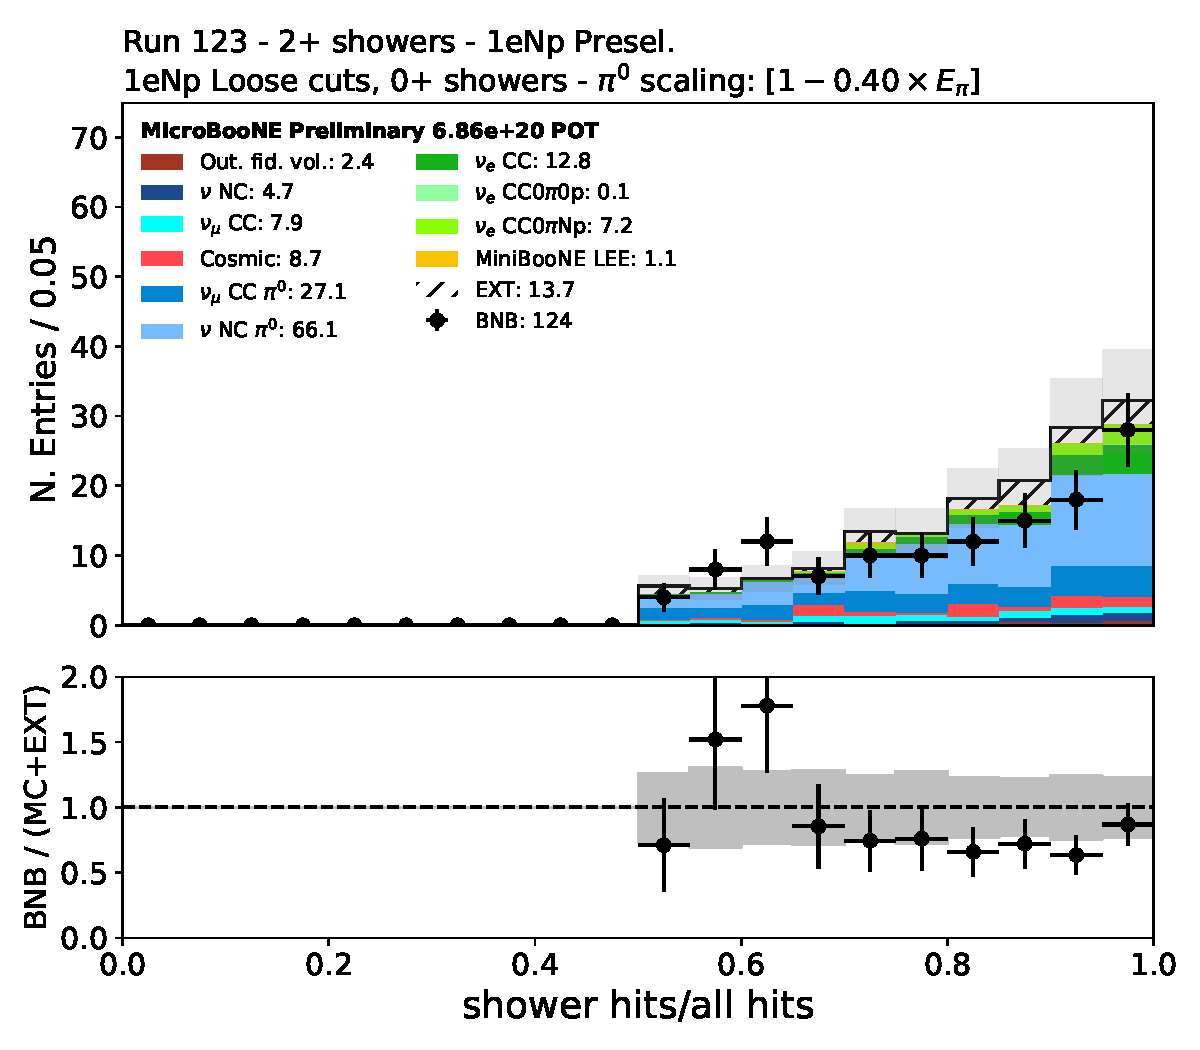
\includegraphics[width=1.00\textwidth]{Sidebands/Figures/1eNp/TwoShower/TwoPShr_NP_NPLAllShr_pi0e040/hits_ratio.pdf}
    %\caption{}
    \end{subfigure}
    \begin{subfigure}{0.45\textwidth}
    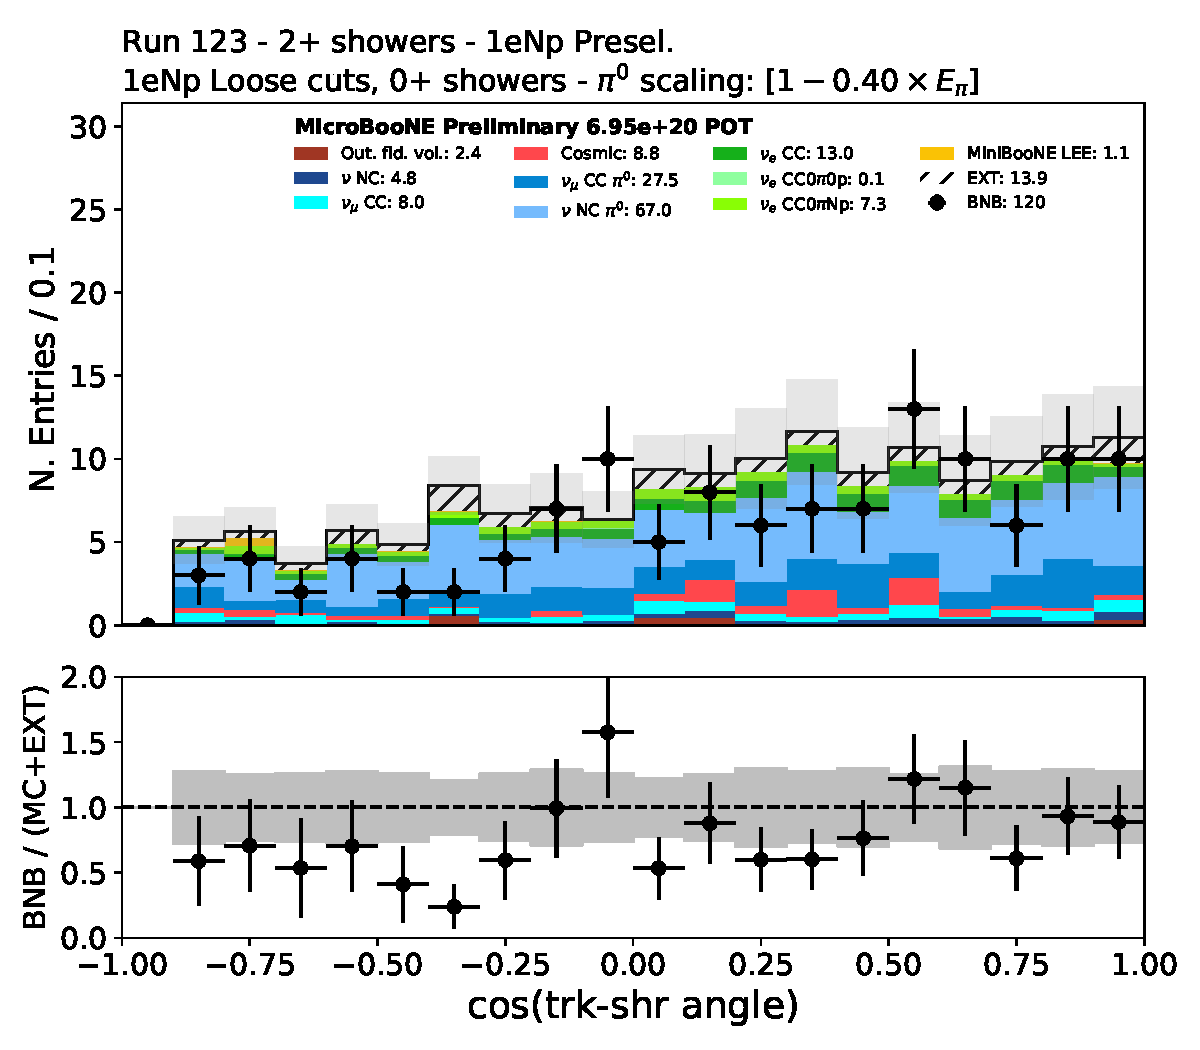
\includegraphics[width=1.00\textwidth]{Sidebands/Figures/1eNp/TwoShower/TwoPShr_NP_NPLAllShr_pi0e040/tksh_angle.pdf}
    %\caption{}
    \end{subfigure} \\
    \begin{subfigure}{0.45\textwidth}
    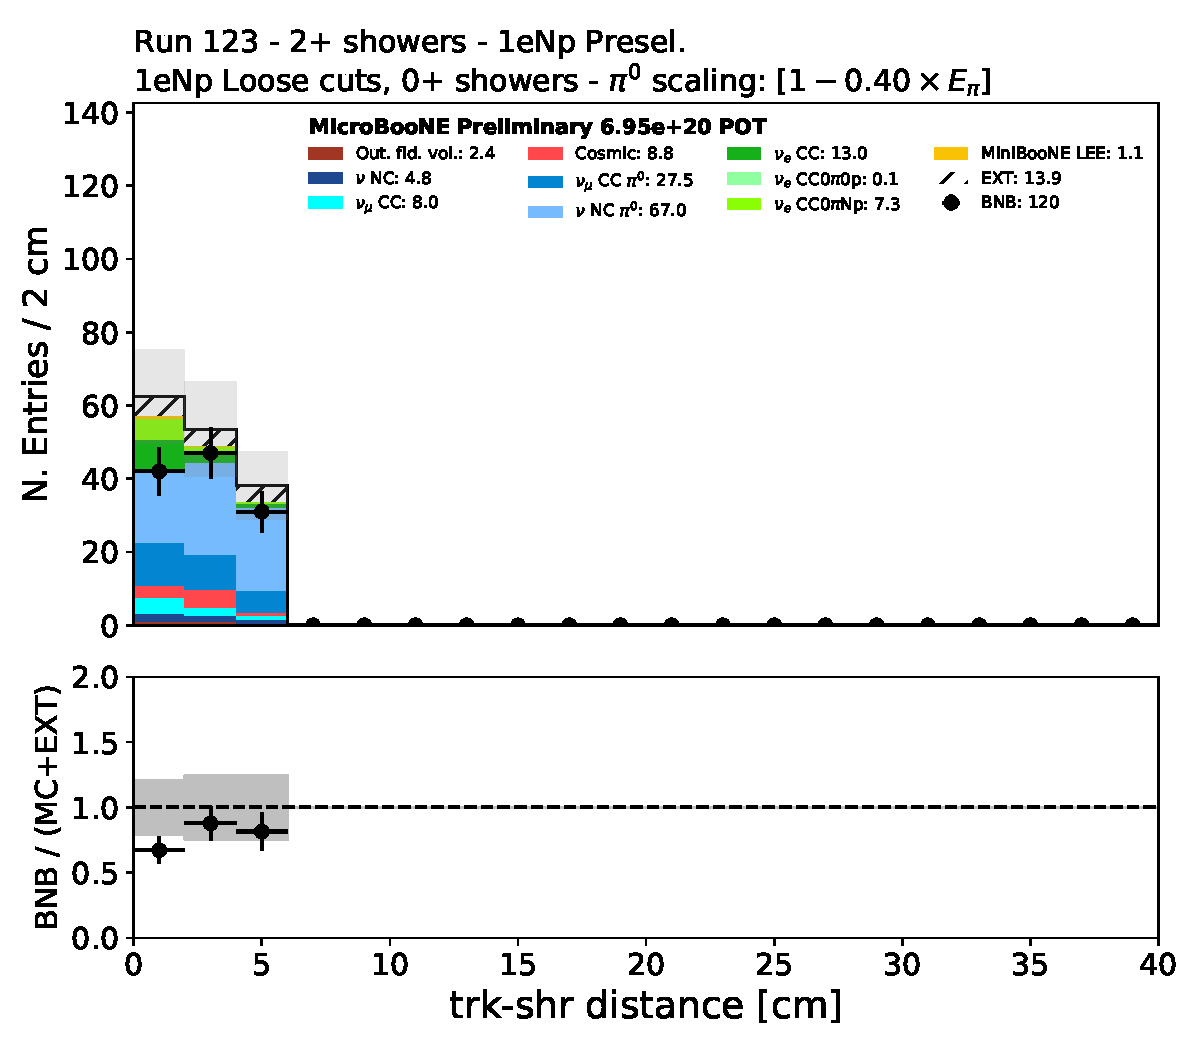
\includegraphics[width=1.00\textwidth]{Sidebands/Figures/1eNp/TwoShower/TwoPShr_NP_NPLAllShr_pi0e040/tksh_distance.pdf}
    %\caption{}
    \end{subfigure}
    \begin{subfigure}{0.45\textwidth}
    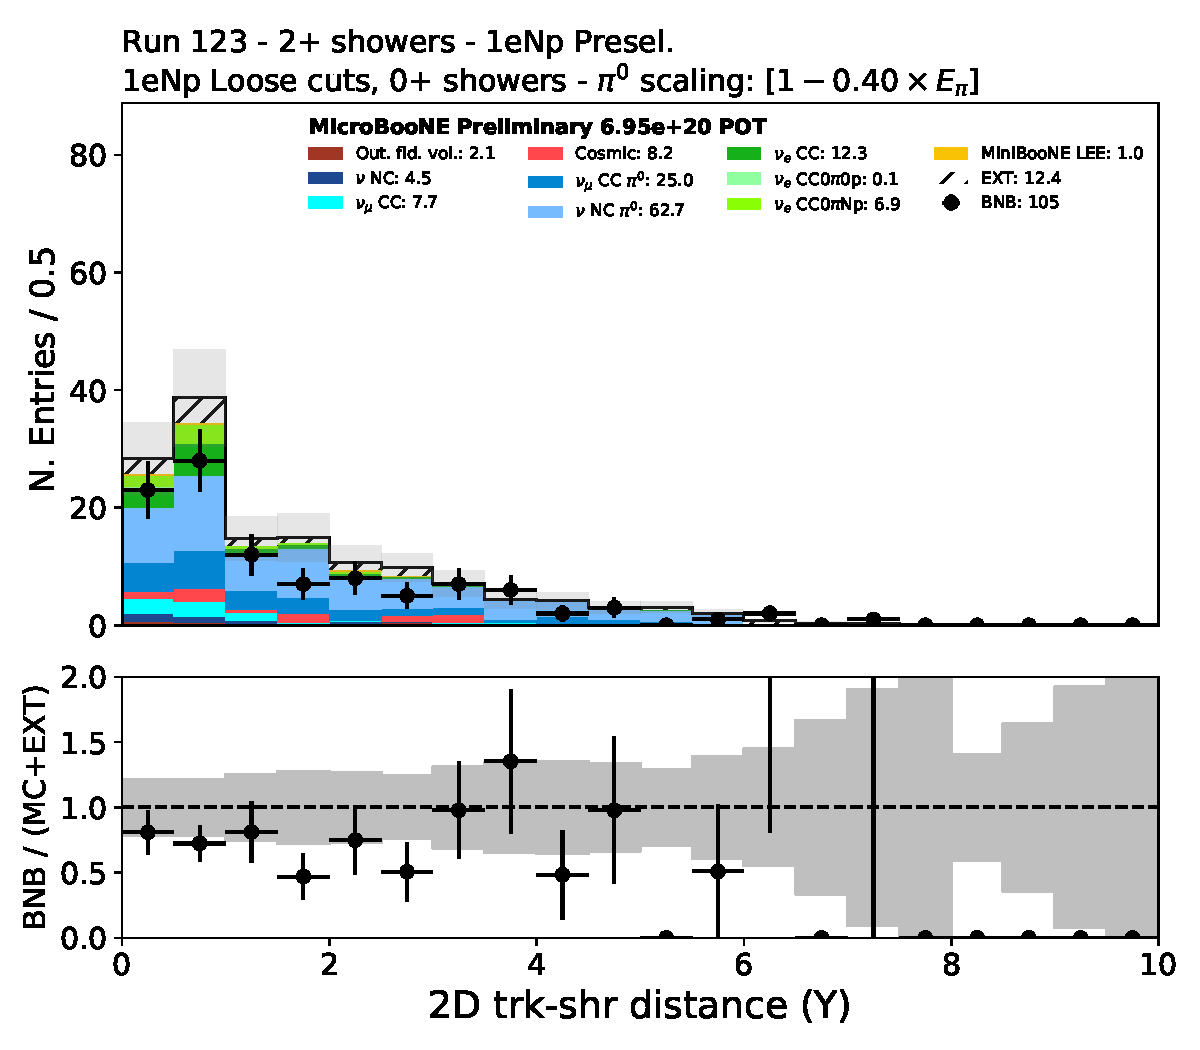
\includegraphics[width=1.00\textwidth]{Sidebands/Figures/1eNp/TwoShower/TwoPShr_NP_NPLAllShr_pi0e040/trkshrhitdist2.pdf}
    %\caption{}
    \end{subfigure}
    \caption{\label{fig:sb:1eNp:twopshr:loose:vars2} Selection variables after \npsel Loose cuts in the 2+ shower sideband.}
    \end{center}
\end{figure}

\begin{figure}[H]
    \begin{center}
    \begin{subfigure}{0.45\textwidth}
    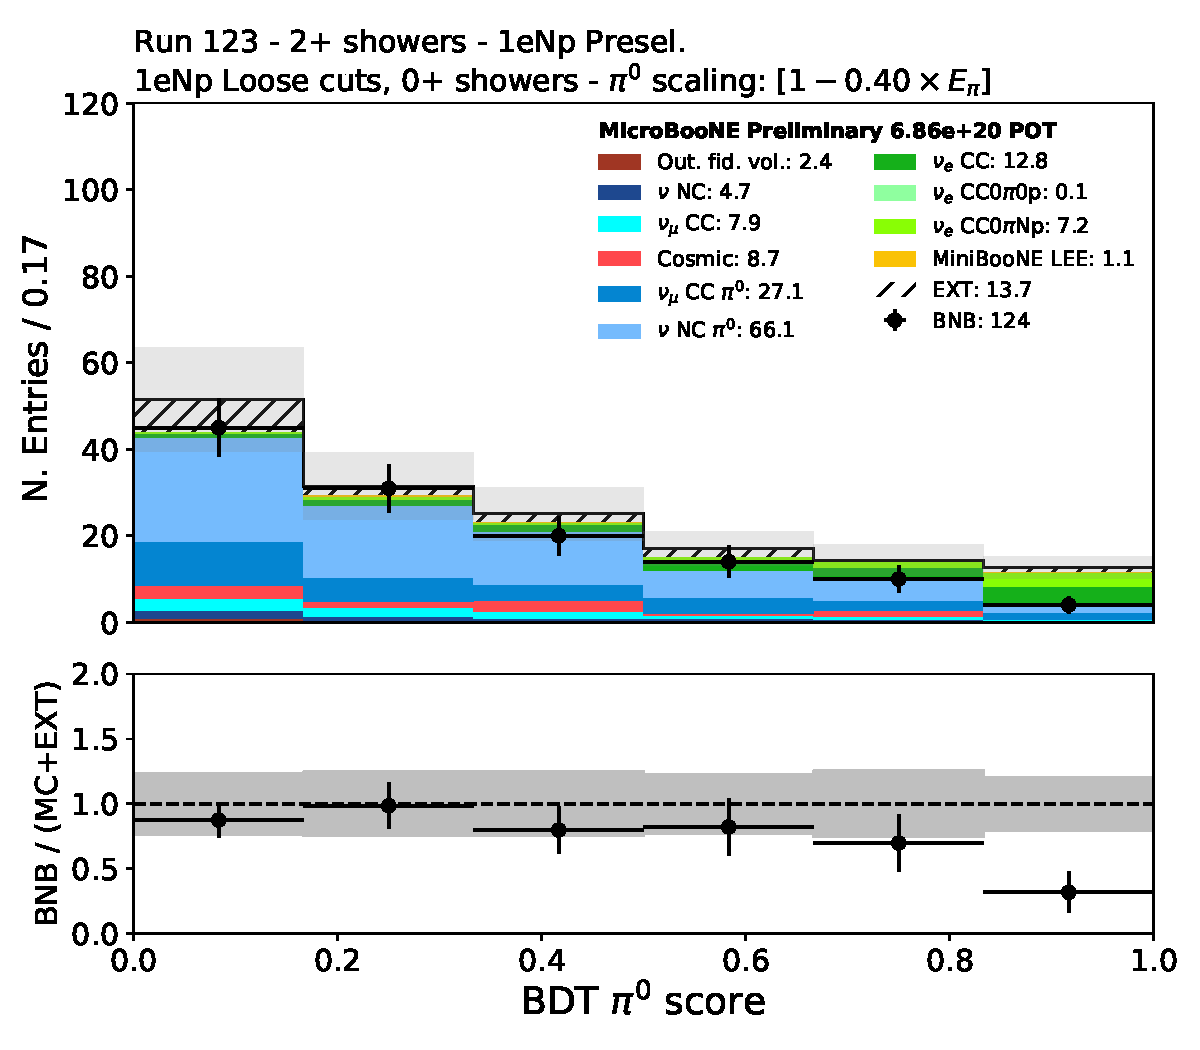
\includegraphics[width=1.00\textwidth]{Sidebands/Figures/1eNp/TwoShower/TwoPShr_NP_NPLAllShr_pi0e040/pi0_score.pdf}
    %\caption{}
    \end{subfigure}
    \begin{subfigure}{0.45\textwidth}
    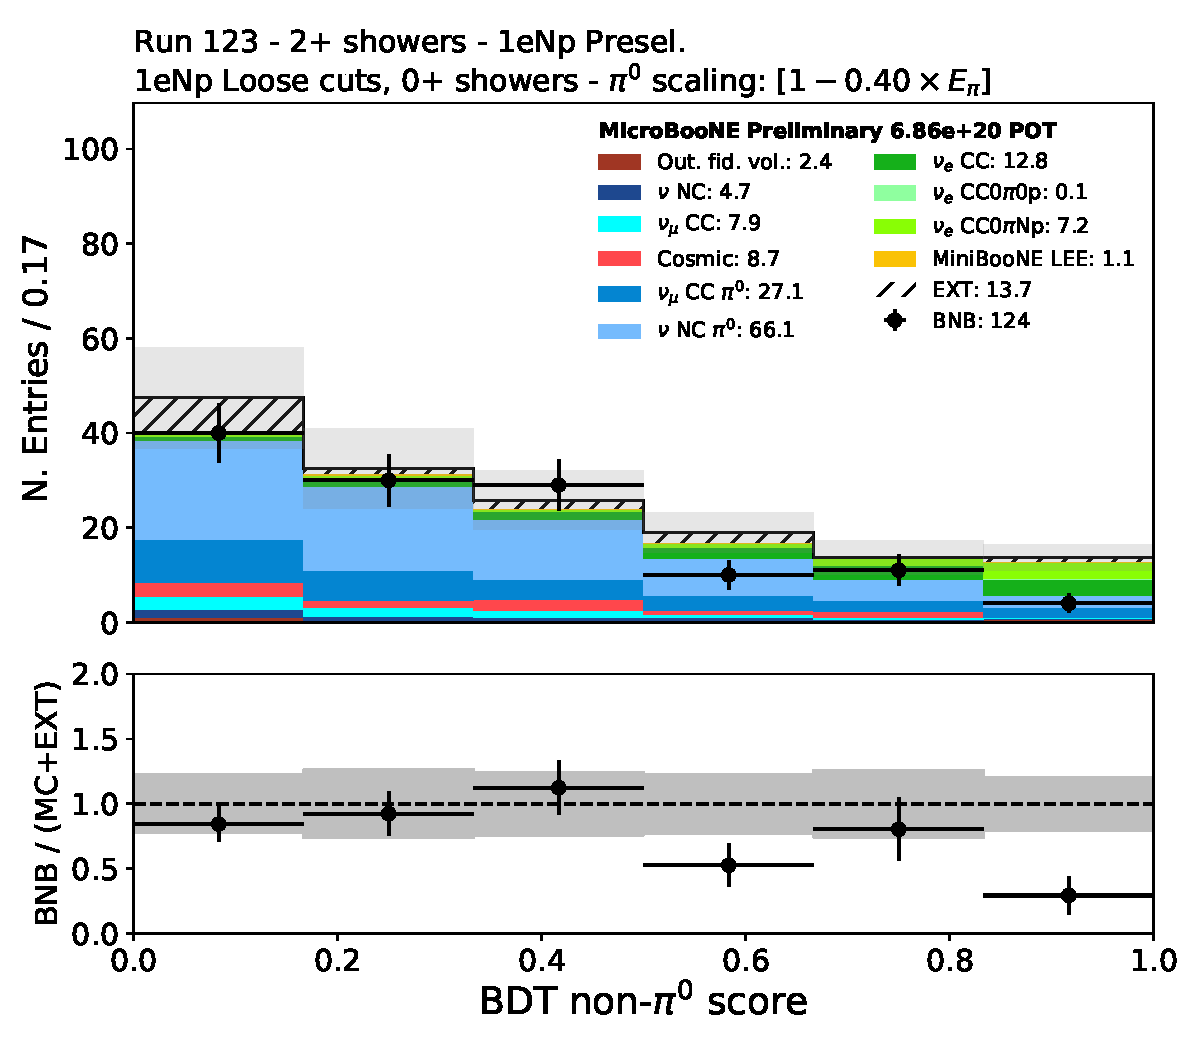
\includegraphics[width=1.00\textwidth]{Sidebands/Figures/1eNp/TwoShower/TwoPShr_NP_NPLAllShr_pi0e040/nonpi0_score.pdf}
    %\caption{}
    \end{subfigure}
    \caption{\label{fig:sb:1eNp:twopshr:loose:bdt} BDT responses after \npsel Loose cuts in the 2+ shower sideband.}
    \end{center}
\end{figure}

\begin{table}[H]
\centering
\setlength{\tabcolsep}{10pt}
\renewcommand{\arraystretch}{1.25}
\begin{tabular}{| c | c | c | c | c | c | c |} 
 \hline
\multirow{3}{*}{variable} & \multicolumn{6}{c|}{p-values} \\
\cline{2-7} & \multicolumn{3}{c|}{pre-selection} & \multicolumn{3}{c|}{loose cuts}  \\
\cline{2-7} & stat-only & diag syst. & covariance & stat-only & diag syst. & covariance \\ \hline
n\_showers\_contained & 0.000 & 0.000 & 0.000 & 0.395 & 0.934 & 0.971 \\ \hline
n\_tracks\_contained & 0.856 & 1.000 & 0.926 & 0.086 & 0.587 & 0.731 \\ \hline
reco\_e & 0.001 & 0.999 & 0.487 & 0.103 & 0.649 & 0.670 \\ \hline
hits\_ratio & 0.318 & 1.000 & 0.575 & 0.081 & 0.589 & 0.529 \\ \hline
CosmicIPAll3D & 0.127 & 1.000 & 0.303 & 0.005 & 0.289 & 0.327 \\ \hline
CosmicDirAll3D & 0.057 & 1.000 & 0.161 & 0.014 & 0.367 & 0.271 \\ \hline
trkfit & 0.077 & 0.997 & 0.367 & 0.013 & 0.412 & 0.250 \\ \hline
shrmoliereavg & 0.415 & 1.000 & 0.759 & 0.115 & 0.579 & 0.731 \\ \hline
shr\_score & 0.319 & 1.000 & 0.625 & 0.041 & 0.584 & 0.578 \\ \hline
subcluster & 0.000 & 0.572 & 0.051 & 0.566 & 0.936 & 0.975 \\ \hline
secondshower\_Y\_nhit & 0.185 & 0.992 & 0.546 & 0.113 & 0.645 & 0.653 \\ \hline
secondshower\_Y\_dot & 0.583 & 1.000 & 0.853 & 0.650 & 0.971 & 0.972 \\ \hline
anglediff\_Y & 0.000 & 0.994 & 0.001 & 0.222 & 0.836 & 0.802 \\ \hline
secondshower\_Y\_vtxdist & 0.001 & 0.999 & 0.019 & 0.490 & 0.942 & 0.972 \\ \hline
shr\_tkfit\_dedx\_max & 0.000 & 0.983 & 0.015 & 0.309 & 0.882 & 0.886 \\ \hline
shr\_trk\_sce\_start\_y & 0.431 & 1.000 & 0.715 & 0.001 & 0.097 & 0.080 \\ \hline
shr\_trk\_sce\_end\_y & 0.048 & 1.000 & 0.198 & 0.103 & 0.701 & 0.718 \\ \hline
tksh\_angle & 0.570 & 1.000 & 0.756 & 0.095 & 0.615 & 0.630 \\ \hline
trkshrhitdist2 & 0.600 & 1.000 & 0.789 & 0.215 & 0.796 & 0.906 \\ \hline
tksh\_distance & 0.529 & 1.000 & 0.741 & 0.086 & 0.638 & 0.668 \\ \hline
trkpid & 0.000 & 0.000 & 0.000 & 0.000 & 0.000 & 0.000 \\ \hline
nonpi0\_score & 0.163 & 0.846 & 0.412 & 0.053 & 0.406 & 0.507 \\ \hline
pi0\_score & 0.015 & 0.640 & 0.064 & 0.018 & 0.277 & 0.355 \\ \hline

 \end{tabular}
 \caption{\label{tab:LOWPIDppvalues}p-values from the 2+ shower \npsel sideband for input variables to the \npsel in addition to the final BDT scores (\texttt{pi0\_score}, \texttt{nonpi0\_score}) and the reconstructed energy spectrum \texttt{reco\_e}. The three columns show the p-values computed through statistics-only uncertainties (left), with systematics but not accounting for correlations in systematics (center), and finally including the full systematics covariance matrix. Systematics include flux, cross-sections, and re-interaction uncertainties, but not detector uncertainties.}
\end{table}

\subsection{\npsel Low BDT Sideband}
\label{app:sideband:1eNplowpid}
Figures~\ref{fig:LPID_1eNp_1} through~\ref{fig:LPID_1eNp_5} show data/mc comparison of the \npsel BDT input variables. Table~\ref{tab:LOWPIDppvalues} shows the p-values for these data/mc comparisons.

\begin{figure}[H]
    \centering
    \begin{subfigure}{0.3\textwidth}
    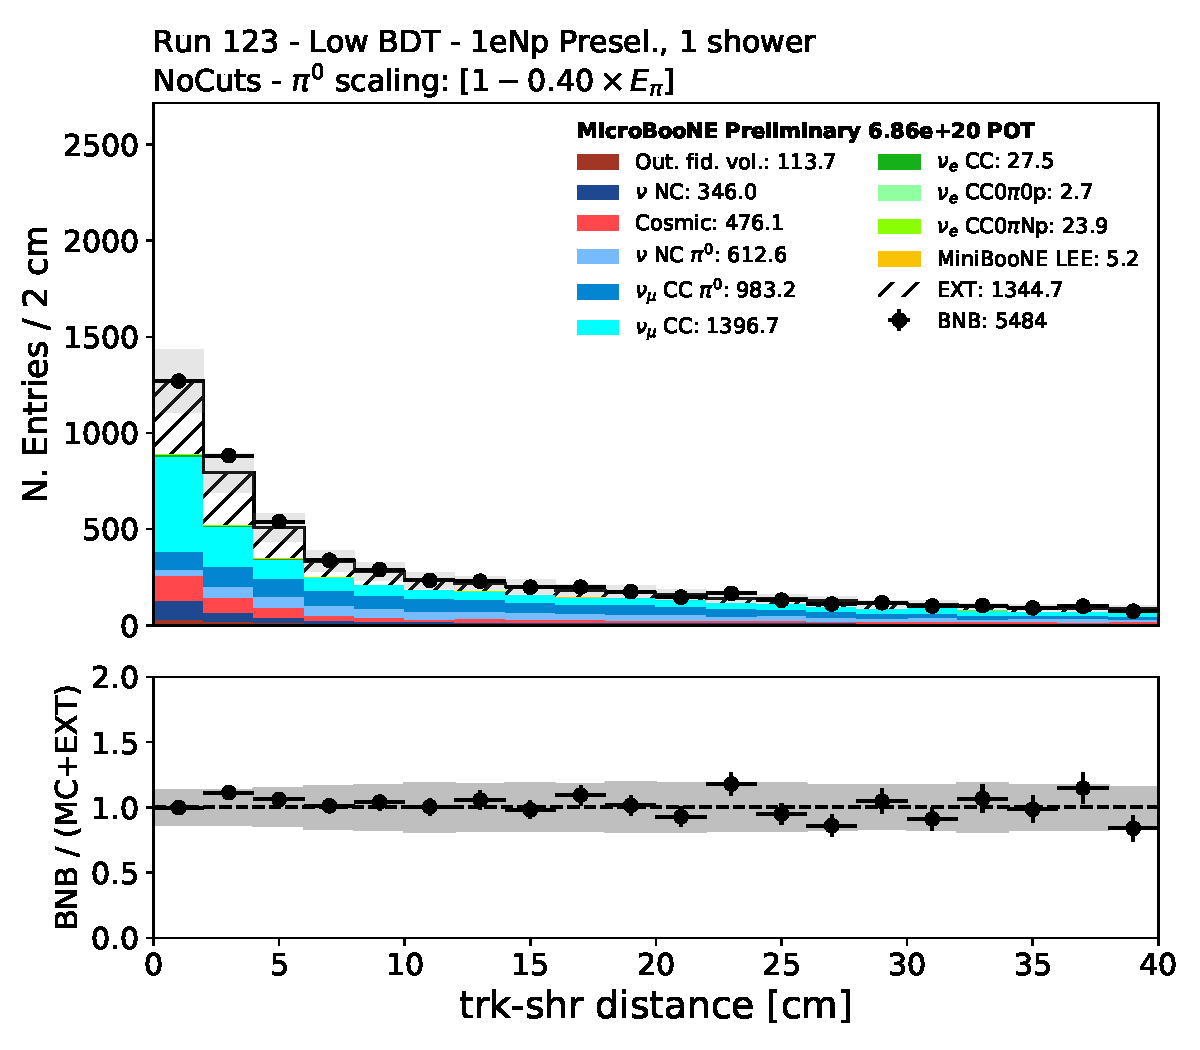
\includegraphics[width=1.0\textwidth]{Sidebands/Figures/1eNp/LPID_NPOneShr_None_pi0e40/tksh_distance.pdf}
    \caption{tksh\_distance}
    \end{subfigure}
    \begin{subfigure}{0.3\textwidth}
    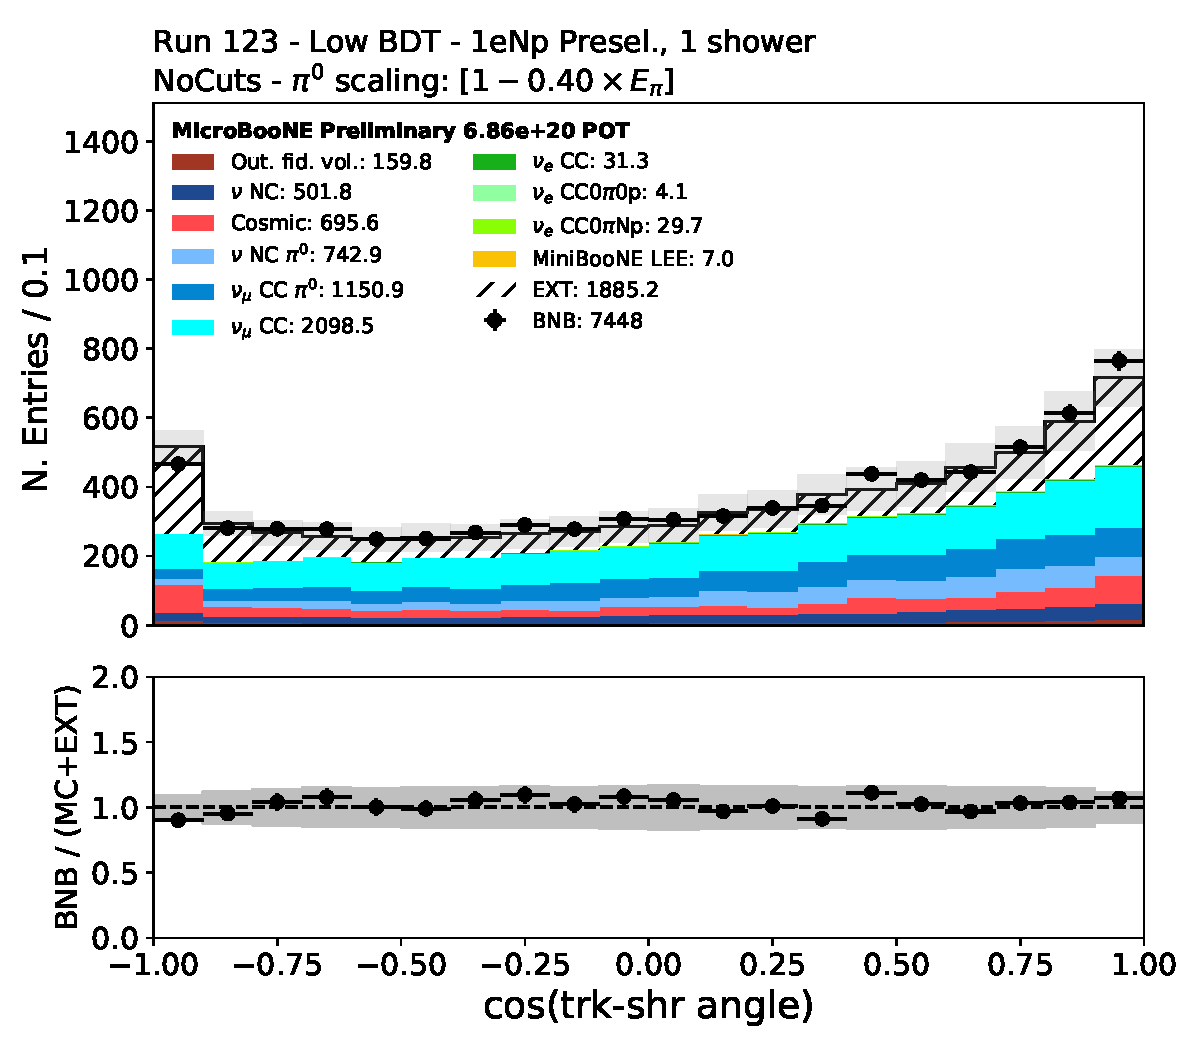
\includegraphics[width=1.0\textwidth]{Sidebands/Figures/1eNp/LPID_NPOneShr_None_pi0e40/tksh_angle.pdf}
    \caption{tksh\_angle}
    \end{subfigure}
    \begin{subfigure}{0.3\textwidth}
    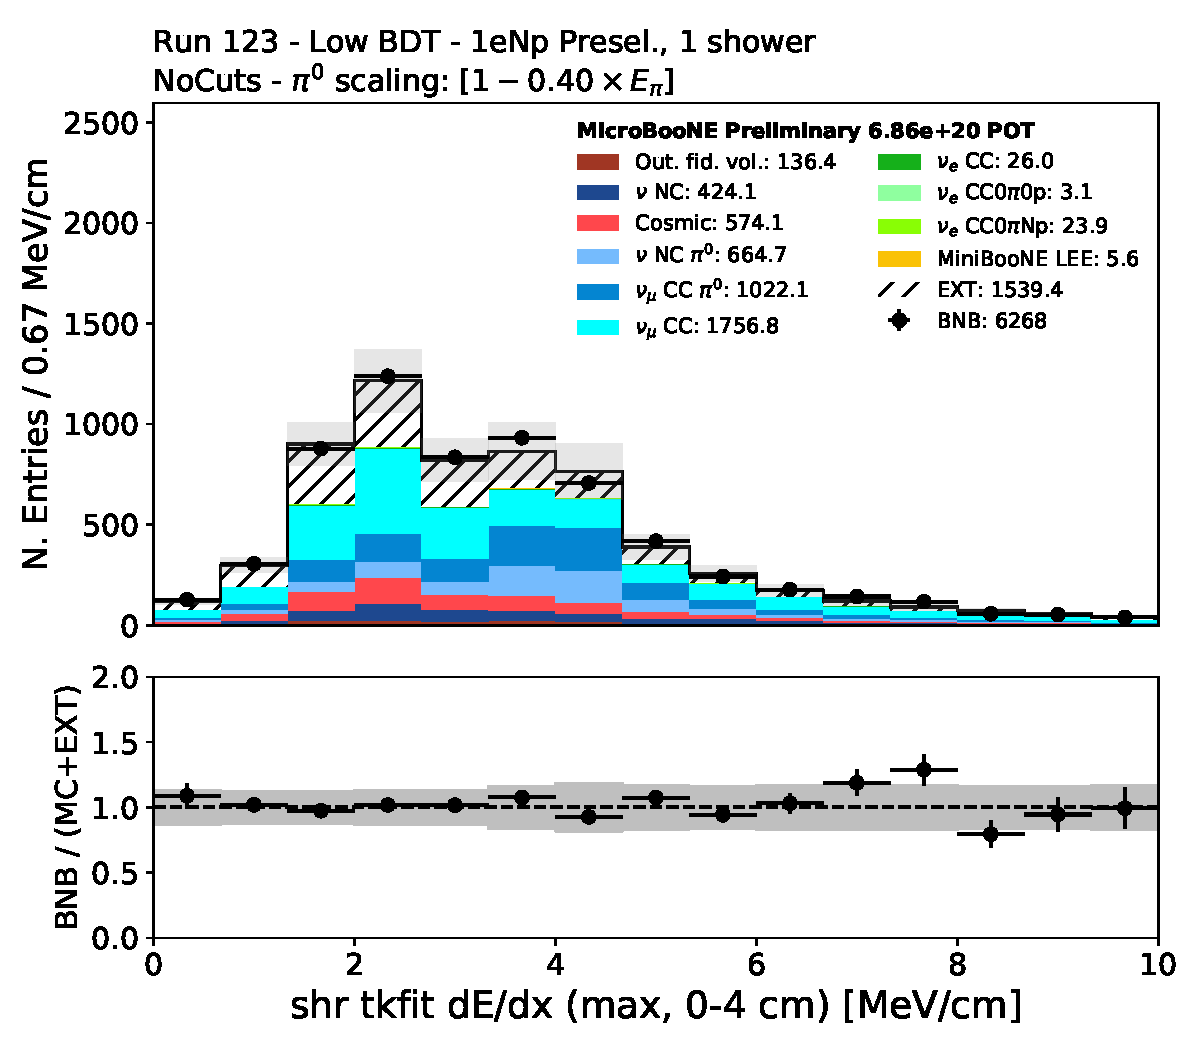
\includegraphics[width=1.0\textwidth]{Sidebands/Figures/1eNp/LPID_NPOneShr_None_pi0e40/shr_tkfit_dedx_max.pdf}
    \caption{shr\_tkfit\_dedx\_max}
    \end{subfigure}
    \caption{} 
    \label{fig:LPID_1eNp_1}
\end{figure}

\begin{figure}[H]
    \centering
    \begin{subfigure}{0.3\textwidth}
    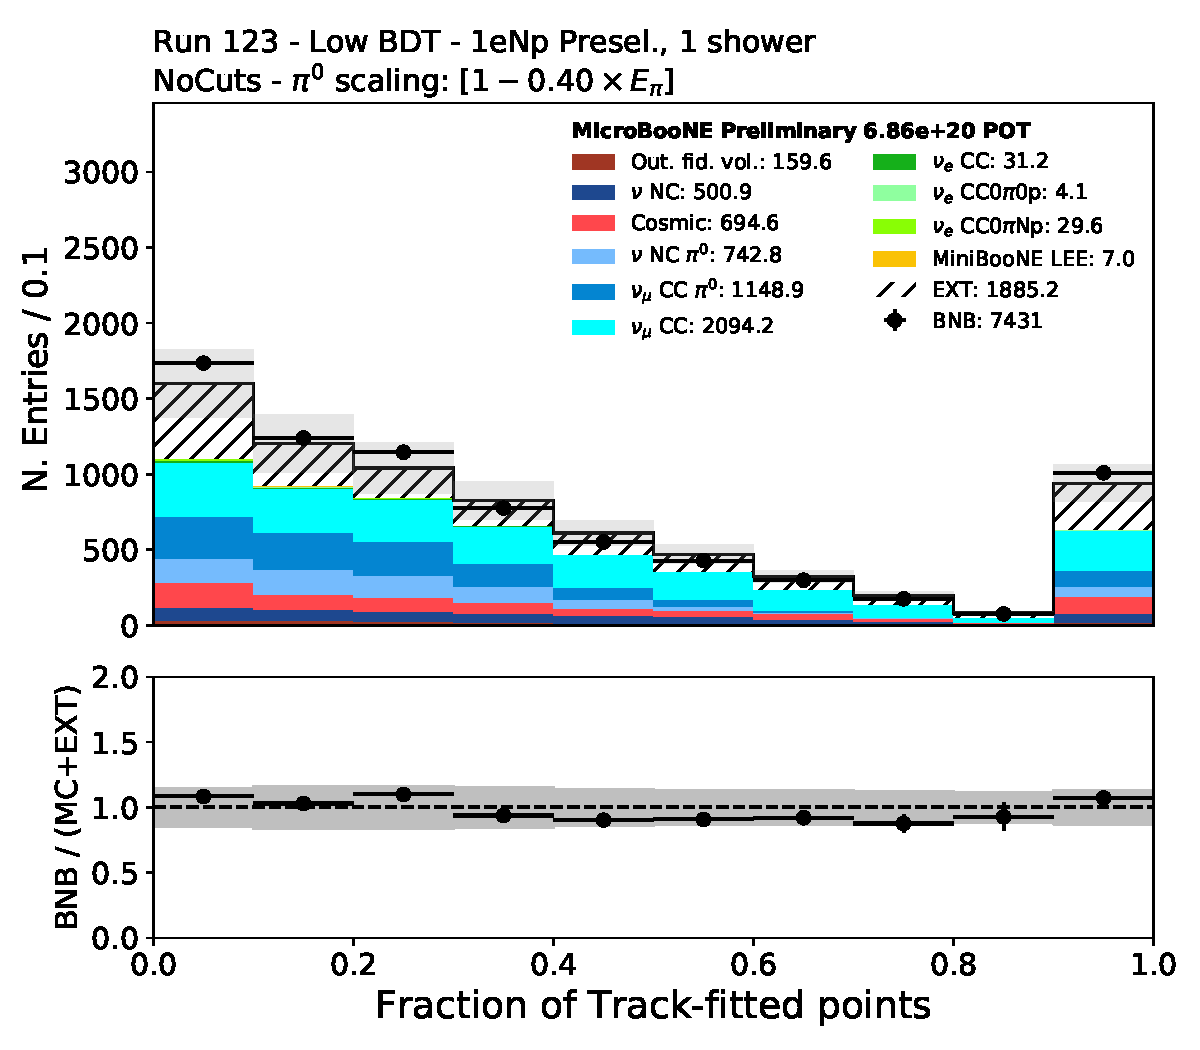
\includegraphics[width=1.0\textwidth]{Sidebands/Figures/1eNp/LPID_NPOneShr_None_pi0e40/trkfit.pdf}
    \caption{trkfit}
    \end{subfigure}
    \begin{subfigure}{0.3\textwidth}
    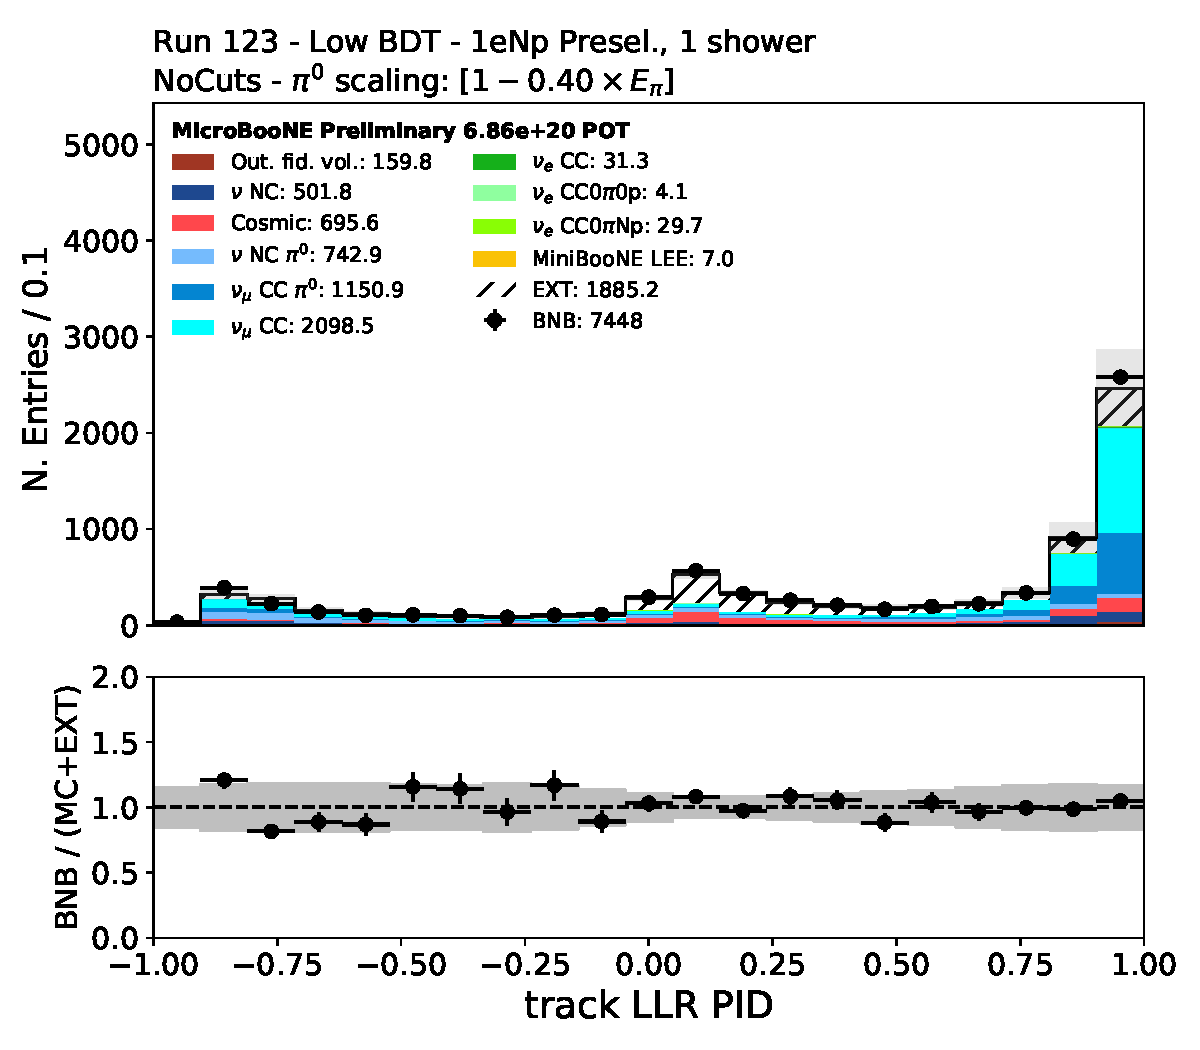
\includegraphics[width=1.0\textwidth]{Sidebands/Figures/1eNp/LPID_NPOneShr_None_pi0e40/trkpid.pdf}
    \caption{trkpid}
    \end{subfigure}
    \begin{subfigure}{0.3\textwidth}
    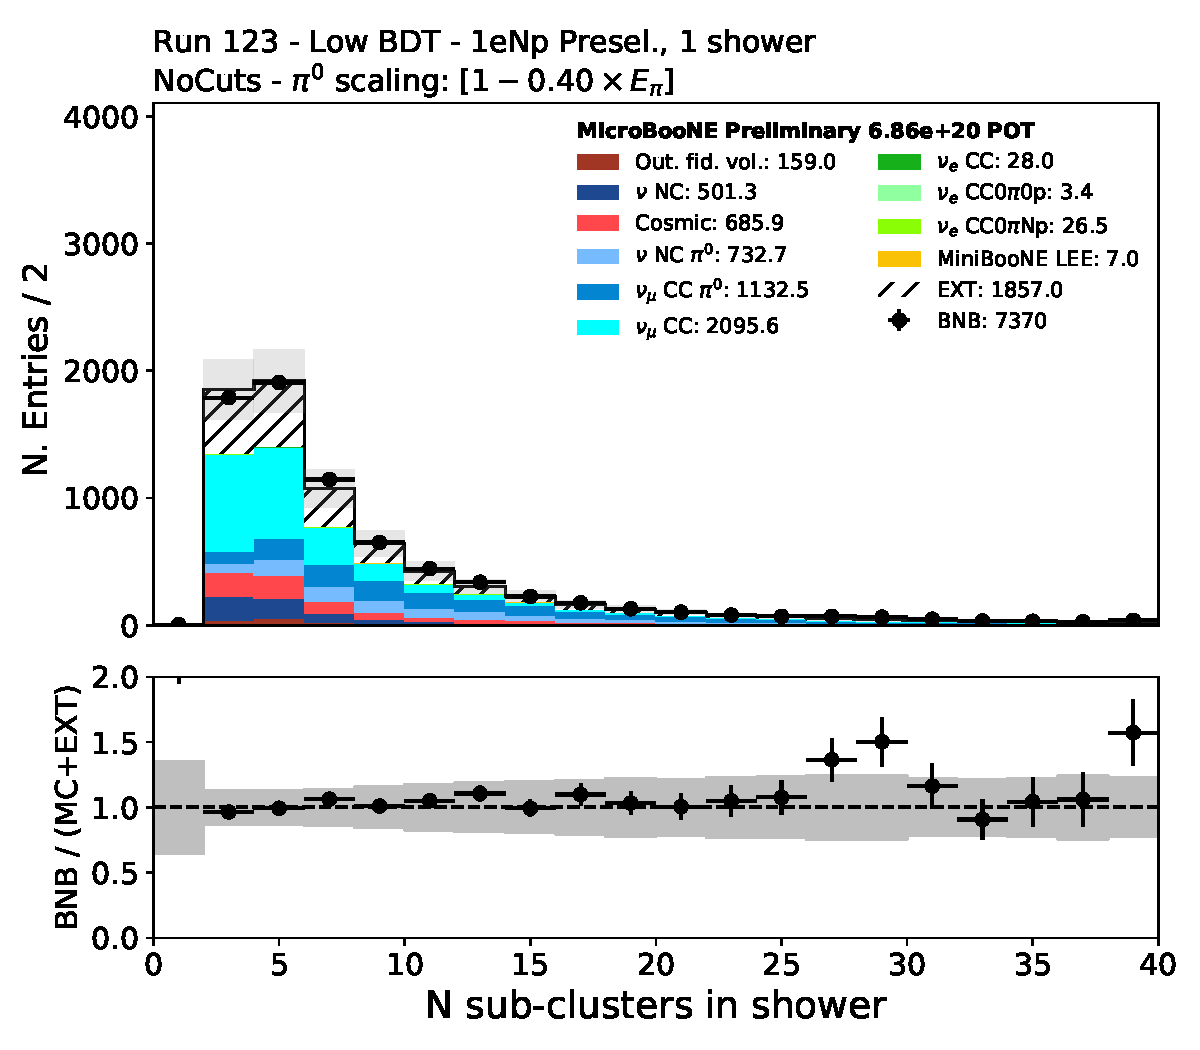
\includegraphics[width=1.0\textwidth]{Sidebands/Figures/1eNp/LPID_NPOneShr_None_pi0e40/subcluster.pdf}
    \caption{subcluster}
    \end{subfigure}
    \caption{} 
    \label{fig:LPID_1eNp_2}
\end{figure}

\begin{figure}[H]
    \centering
    \begin{subfigure}{0.3\textwidth}
    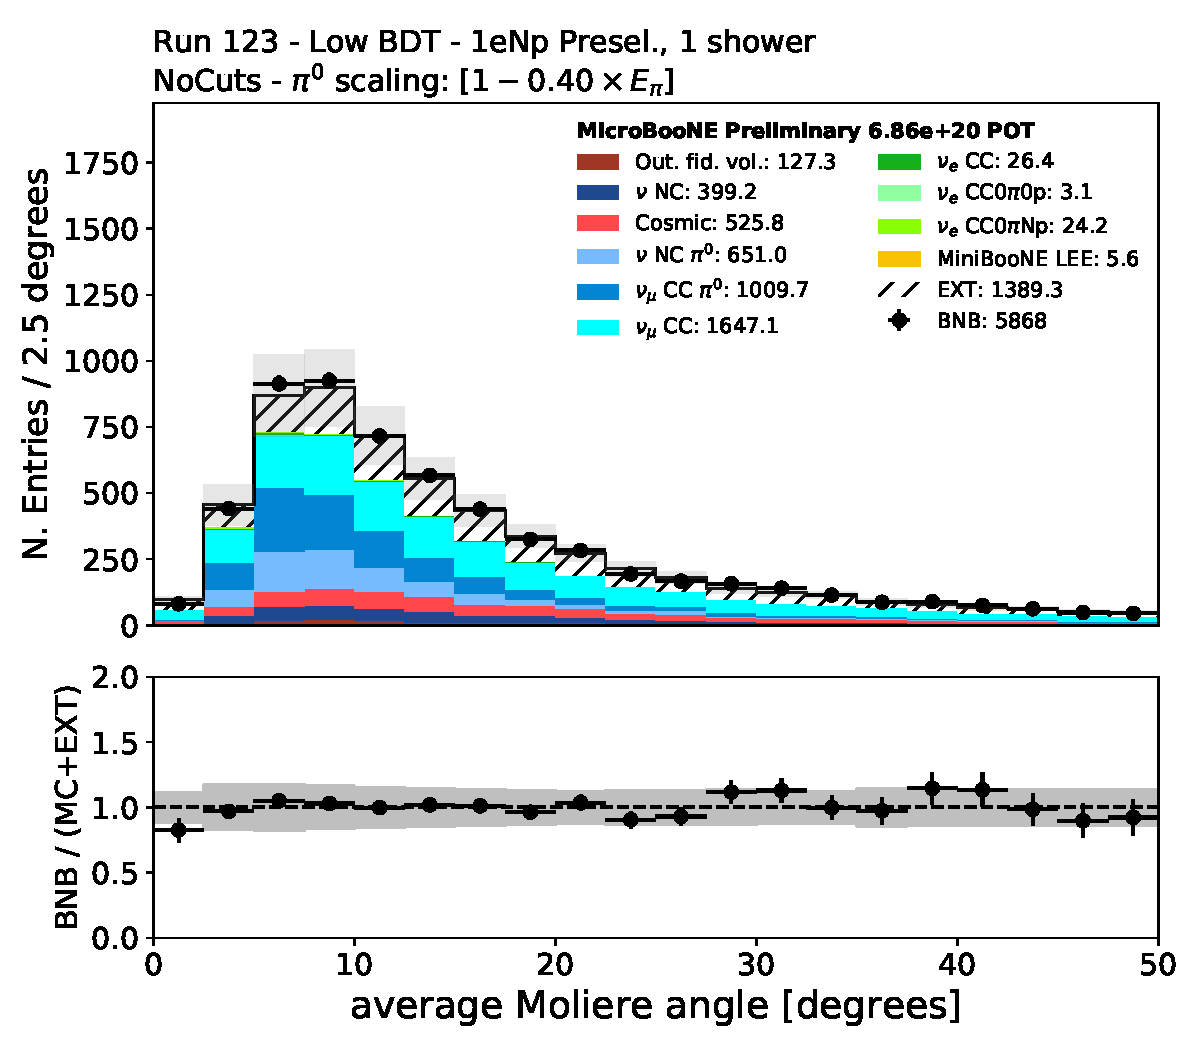
\includegraphics[width=1.0\textwidth]{Sidebands/Figures/1eNp/LPID_NPOneShr_None_pi0e40/shrmoliereavg.pdf}
    \caption{shrmoliereavg}
    \end{subfigure}
    \begin{subfigure}{0.3\textwidth}
    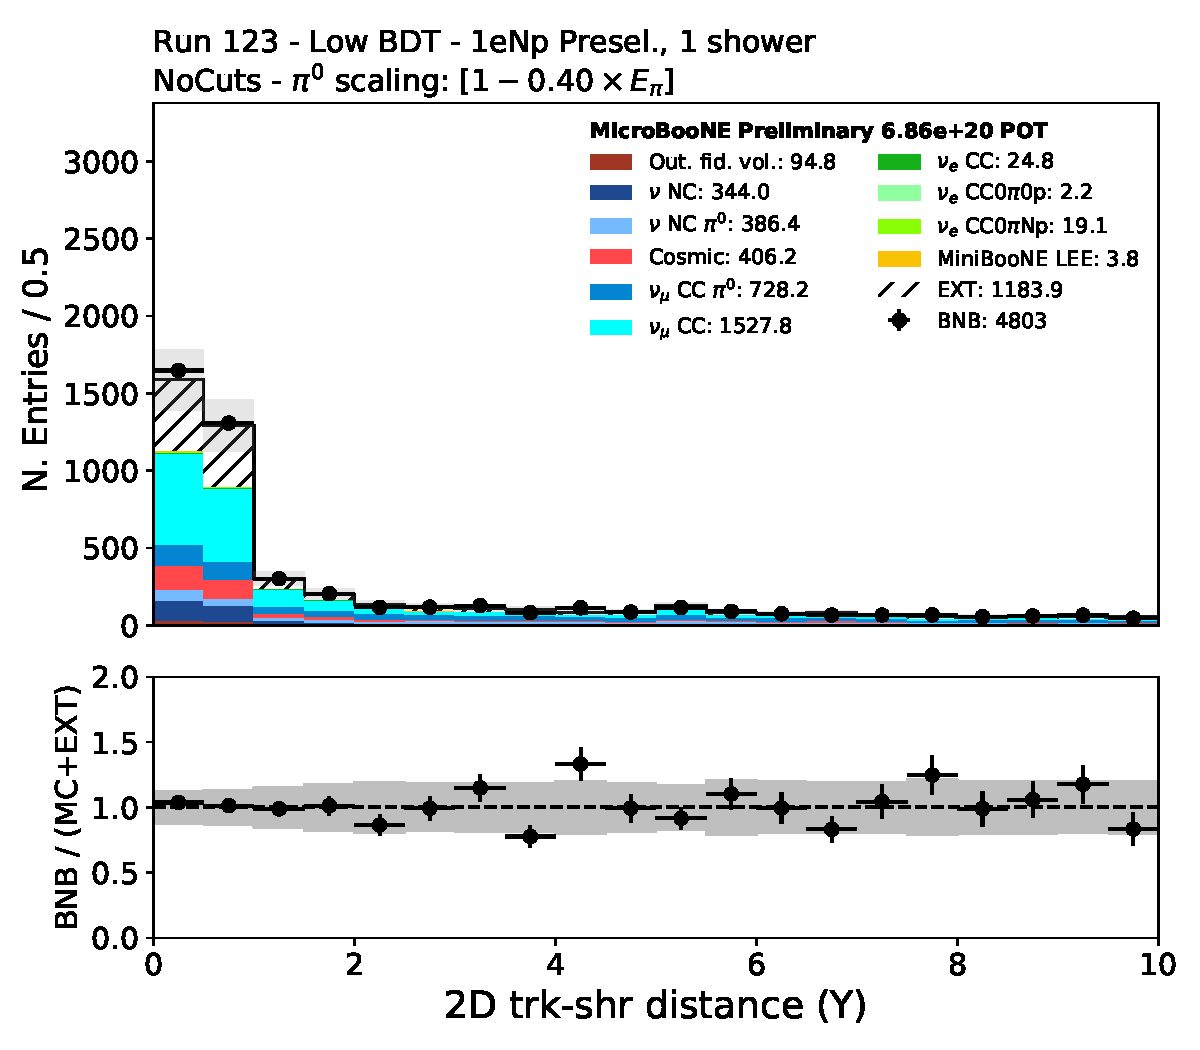
\includegraphics[width=1.0\textwidth]{Sidebands/Figures/1eNp/LPID_NPOneShr_None_pi0e40/trkshrhitdist2.pdf}
    \caption{tkshrhitdist2}
    \end{subfigure}
    \begin{subfigure}{0.3\textwidth}
    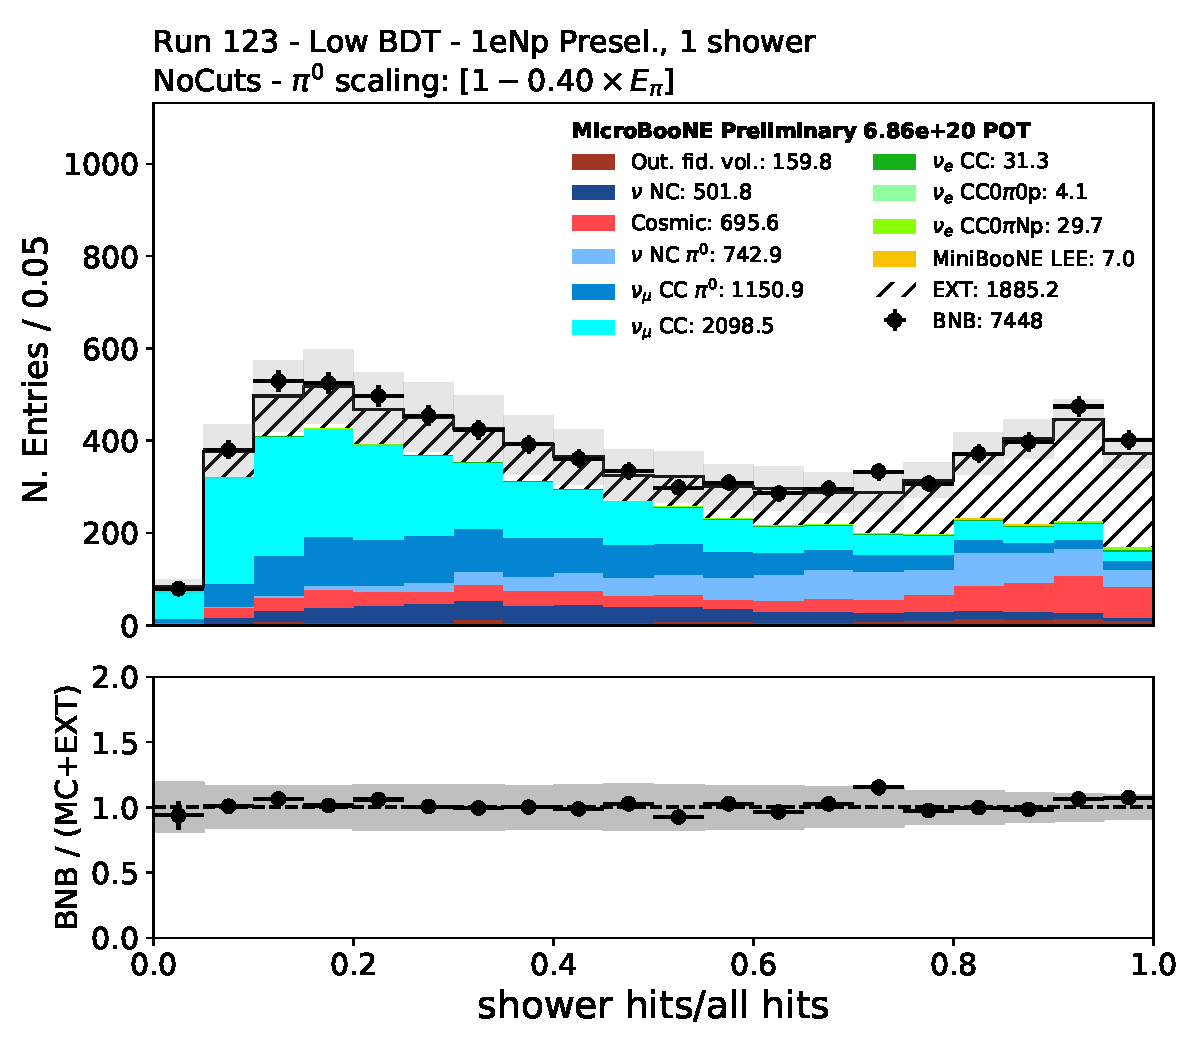
\includegraphics[width=1.0\textwidth]{Sidebands/Figures/1eNp/LPID_NPOneShr_None_pi0e40/hits_ratio.pdf}
    \caption{hits\_ratio}
    \end{subfigure}
    \caption{} 
    \label{fig:LPID_1eNp_3}
\end{figure}

\begin{figure}[H]
    \centering
    \begin{subfigure}{0.3\textwidth}
    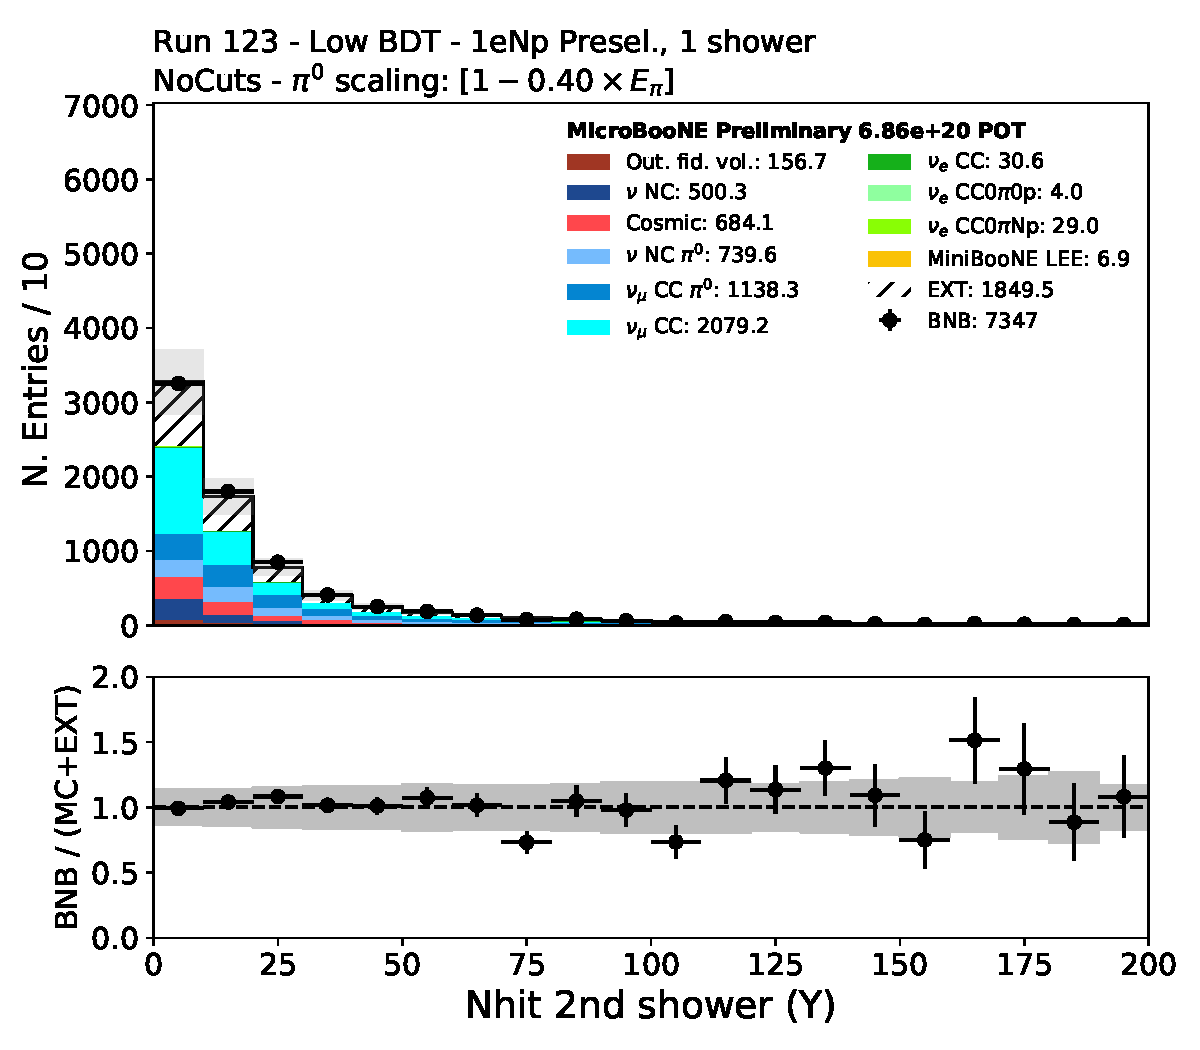
\includegraphics[width=1.0\textwidth]{Sidebands/Figures/1eNp/LPID_NPOneShr_None_pi0e40/secondshower_Y_nhit.pdf}
    \caption{secondshower\_Y\_nhit}
    \end{subfigure}
    \begin{subfigure}{0.3\textwidth}
    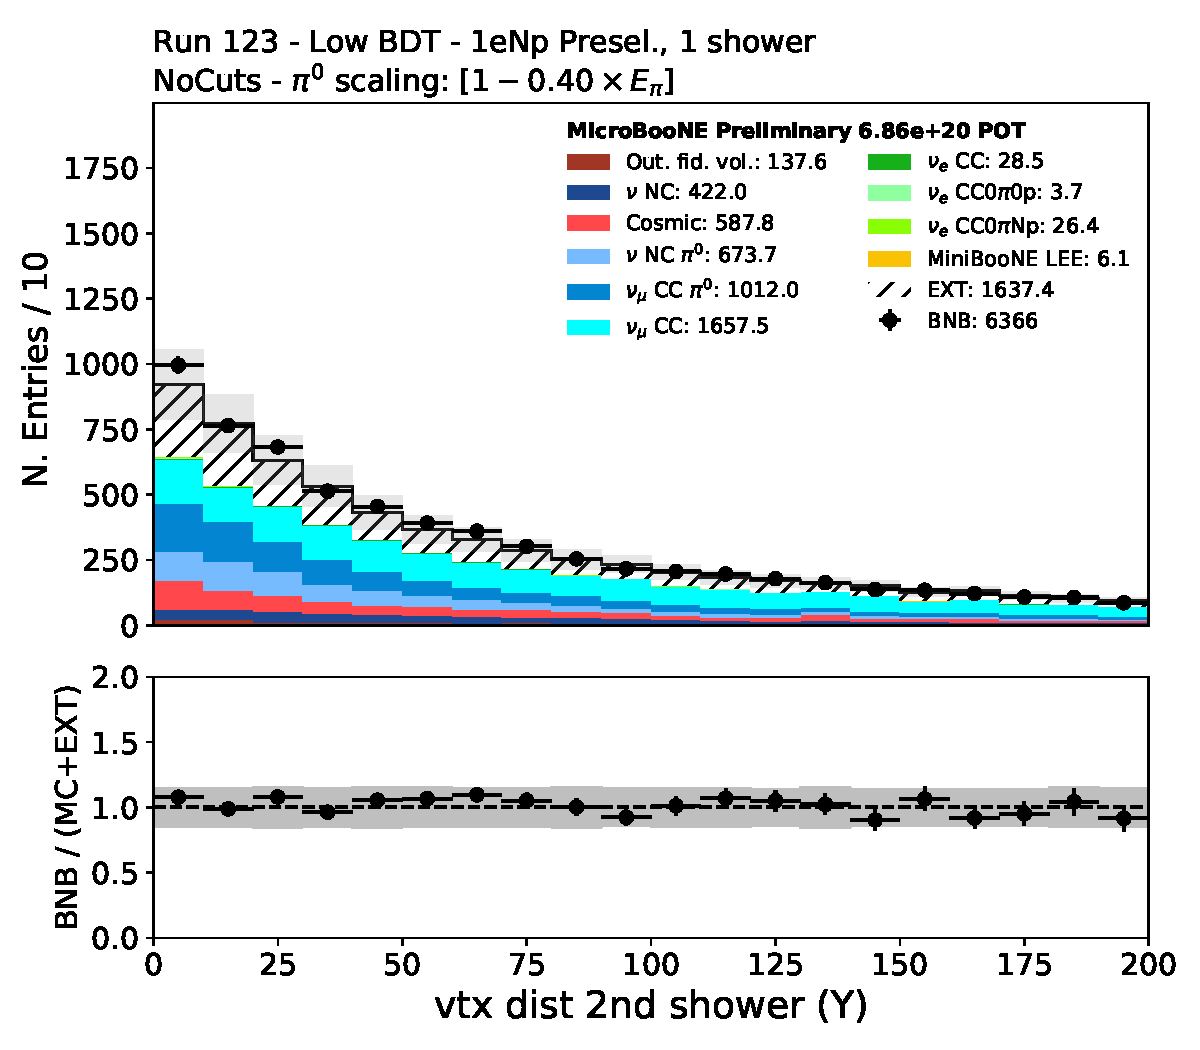
\includegraphics[width=1.0\textwidth]{Sidebands/Figures/1eNp/LPID_NPOneShr_None_pi0e40/secondshower_Y_vtxdist.pdf}
    \caption{secondshower\_Y\_vtxdist}
    \end{subfigure}
    \begin{subfigure}{0.3\textwidth}
    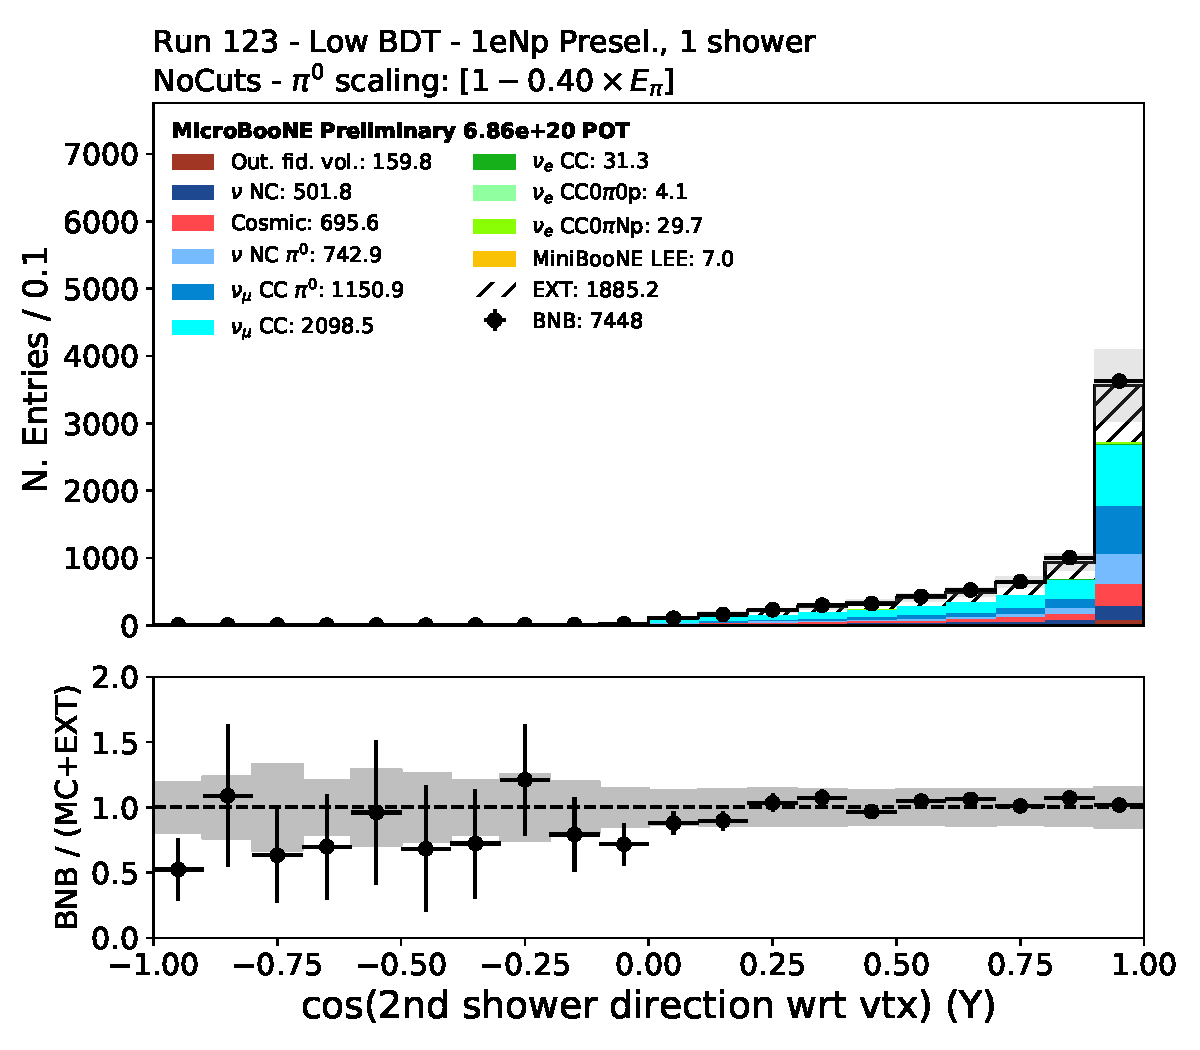
\includegraphics[width=1.0\textwidth]{Sidebands/Figures/1eNp/LPID_NPOneShr_None_pi0e40/secondshower_Y_dot.pdf}
    \caption{secondshower\_Y\_dot}
    \end{subfigure}
    \caption{} 
    \label{fig:LPID_1eNp_4}
\end{figure}

\begin{figure}[H]
    \centering
    \begin{subfigure}{0.3\textwidth}
    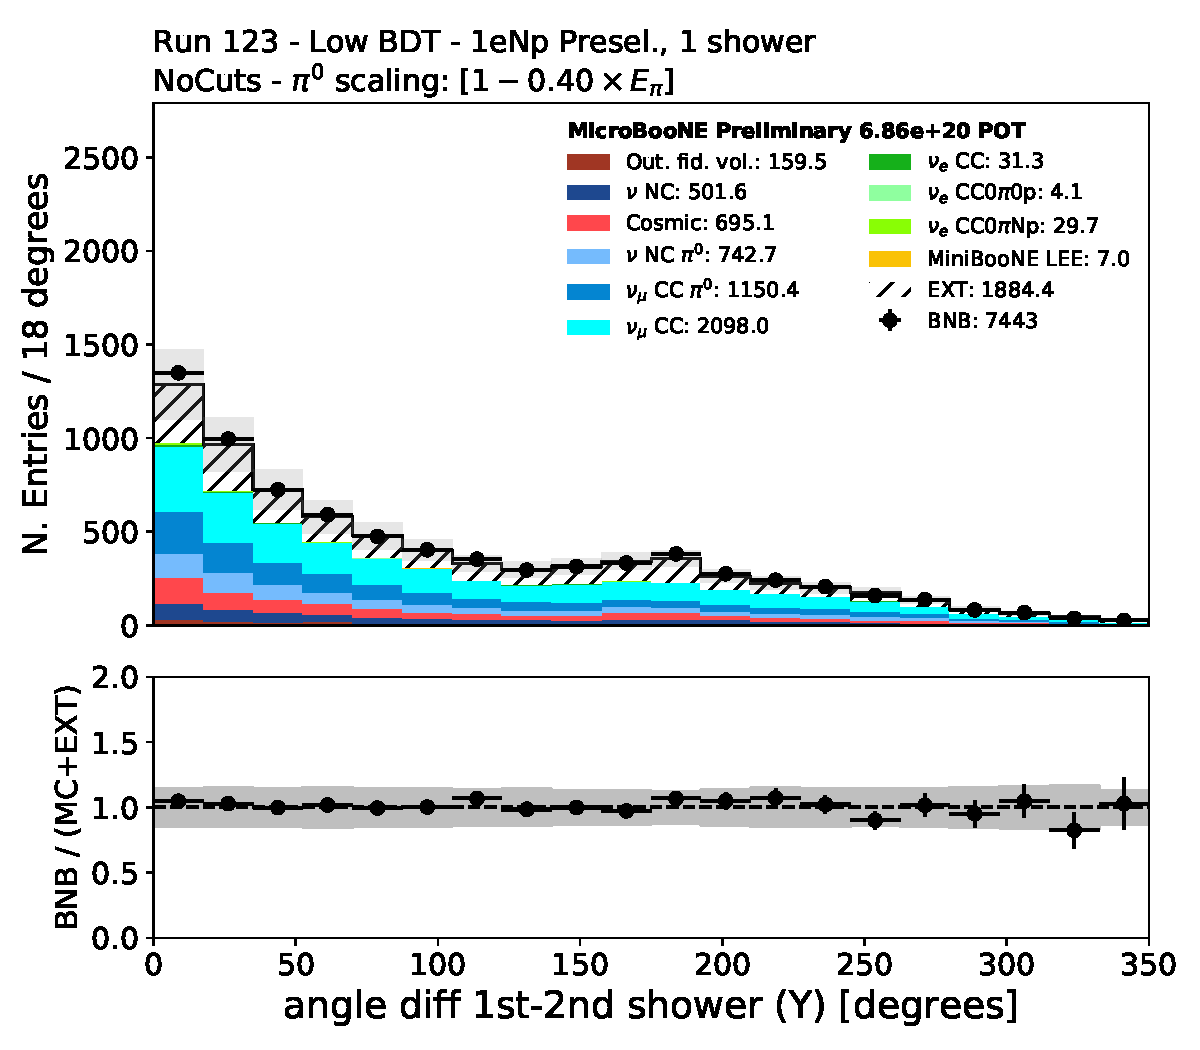
\includegraphics[width=1.0\textwidth]{Sidebands/Figures/1eNp/LPID_NPOneShr_None_pi0e40/anglediff_Y.pdf}
    \caption{anglediff\_Y}
    \end{subfigure}
    \begin{subfigure}{0.3\textwidth}
    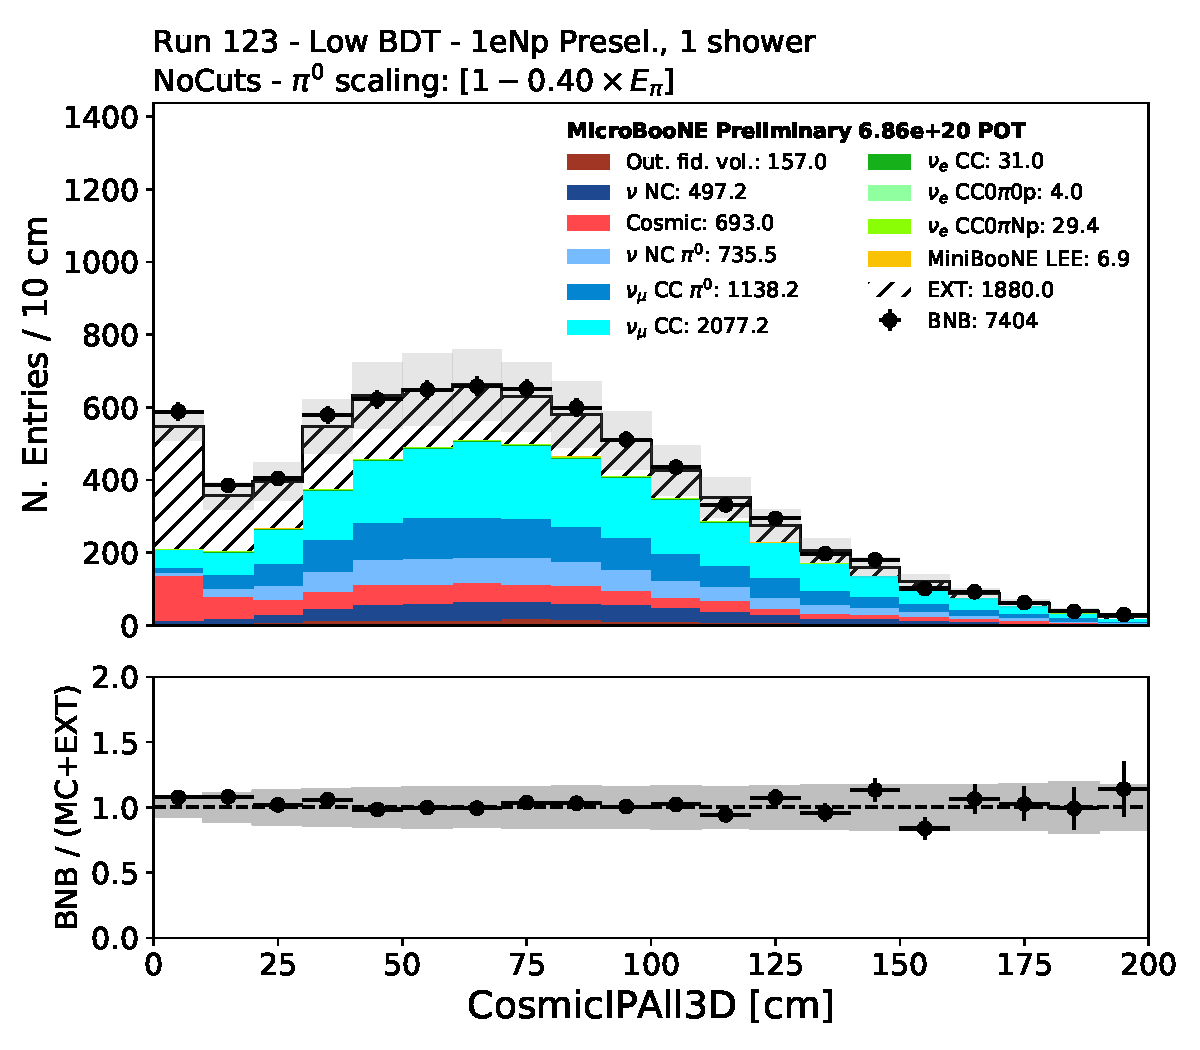
\includegraphics[width=1.0\textwidth]{Sidebands/Figures/1eNp/LPID_NPOneShr_None_pi0e40/CosmicIPAll3D.pdf}
    \caption{CosmicIPAll3D}
    \end{subfigure}
    \begin{subfigure}{0.3\textwidth}
    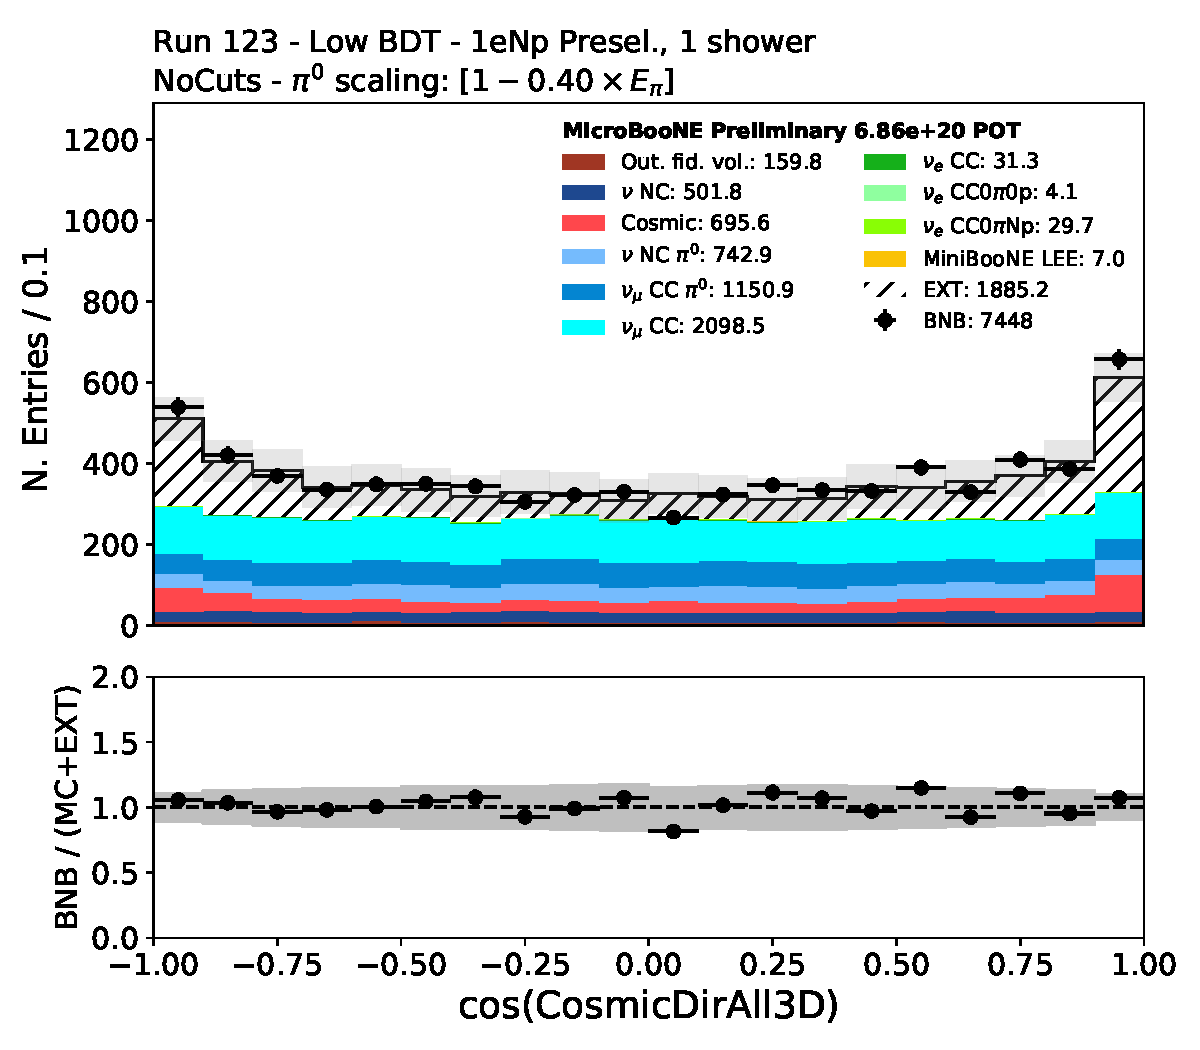
\includegraphics[width=1.0\textwidth]{Sidebands/Figures/1eNp/LPID_NPOneShr_None_pi0e40/CosmicDirAll3D.pdf}
    \caption{CosmidDirAll3D}
    \end{subfigure}
    \caption{} 
    \label{fig:LPID_1eNp_5}
\end{figure}


\begin{table}[H]
\centering
\setlength{\tabcolsep}{10pt}
\renewcommand{\arraystretch}{1.25}
\begin{tabular}{| c | c | c | c | } 
 \hline
\multirow{2}{*}{variable} & \multicolumn{3}{c|}{p-values} \\
\cline{2-4} & stat-only & diag syst. & full covariance \\ \hline
n\_showers\_contained & 0.100 & 0.892 & 0.892 \\ \hline
n\_tracks\_contained & 0.206 & 0.997 & 0.791 \\ \hline
reco\_e & 0.011 & 0.996 & 0.311 \\ \hline
hits\_ratio & 0.599 & 1.000 & 0.858 \\ \hline
CosmicIPAll3D & 0.506 & 1.000 & 0.822 \\ \hline
CosmicDirAll3D & 0.002 & 1.000 & 0.026 \\ \hline
tksh\_angle & 0.117 & 1.000 & 0.447 \\ \hline
trkshrhitdist2 & 0.038 & 0.995 & 0.138 \\ \hline
tksh\_distance & 0.100 & 1.000 & 0.392 \\ \hline
trkpid & 0.000 & 0.001 & 0.000 \\ \hline
trkfit & 0.000 & 0.969 & 0.026 \\ \hline
shrmoliereavg & 0.577 & 1.000 & 0.829 \\ \hline
shr\_score & 0.008 & 1.000 & 0.874 \\ \hline
subcluster & 0.002 & 0.755 & 0.224 \\ \hline
subcluster & 0.008 & 0.838 & 0.421 \\ \hline
secondshower\_Y\_nhit & 0.045 & 0.973 & 0.263 \\ \hline
secondshower\_Y\_dot & 0.304 & 0.995 & 0.745 \\ \hline
anglediff\_Y & 0.880 & 1.000 & 0.987 \\ \hline
secondshower\_Y\_vtxdist & 0.255 & 1.000 & 0.790 \\ \hline
shr\_tkfit\_dedx\_max & 0.016 & 0.990 & 0.078 \\ \hline
shr\_trk\_sce\_start\_y & 0.029 & 0.934 & 0.153 \\ \hline
shr\_trk\_sce\_end\_y & 0.366 & 1.000 & 0.728 \\ \hline
nonpi0\_score & 0.011 & 0.424 & 0.166 \\ \hline
pi0\_score & 0.036 & 0.159 & 0.155 \\ \hline

 \end{tabular}
 \caption{\label{tab:LOWPIDppvalues}p-values from the low-PID \npsel sideband for input variables to the \npsel in addition to the final BDT scores (\texttt{pi0\_score}, \texttt{nonpi0\_score}) and the reconstructed energy spectrum \texttt{reco\_e}. The three columns show the p-values computed through statistics-only uncertainties (left), with systematics but not accounting for correlations in systematics (center), and finally including the full systematics covariance matrix. Systematics include flux, cross-sections, and re-interaction uncertainties, but not detector uncertainties.}
\end{table}

\subsection{\npsel High Energy Sideband}
\label{app:datasidebandplotdump:nphe}

This section presents data-mc comparisons of selection input distributions as well as event kinematics at different stages in the $\nu_e$ \npsel selection. 
Figures~\ref{fig:HE_1eNp_1} to~\ref{fig:HE_1eNp_5} show all BDT input variables from the HE sideband at pre-selection stage.

\begin{figure}[H]
    \centering
    \begin{subfigure}{0.3\textwidth}
    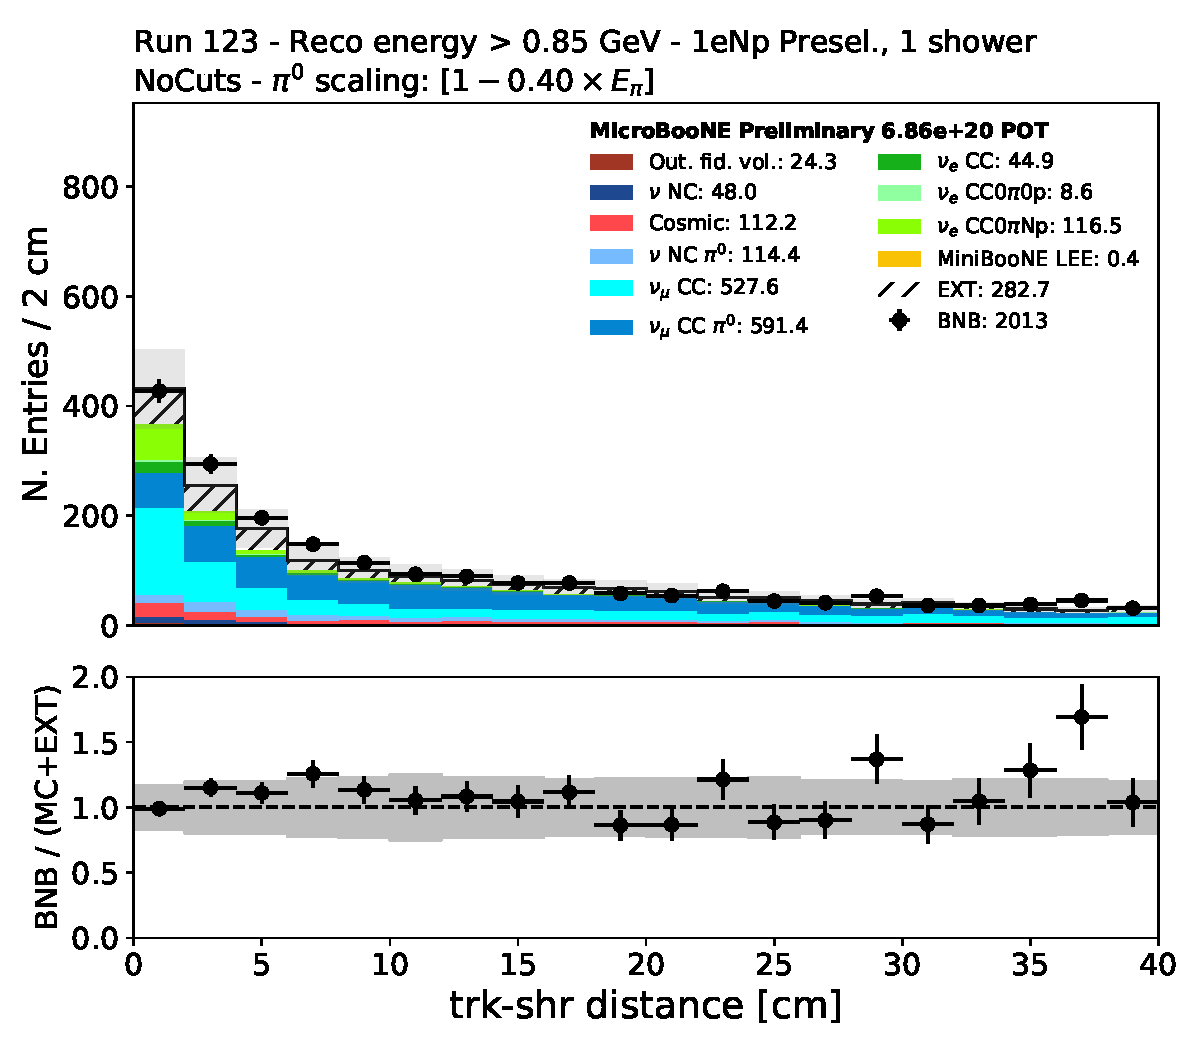
\includegraphics[width=1.0\textwidth]{Sidebands/Figures/1eNp/HighEnergy/HiEext_NPOneShr_None_pi0e040/tksh_distance.pdf}
    \caption{tksh\_distance}
    \end{subfigure}
    \begin{subfigure}{0.3\textwidth}
    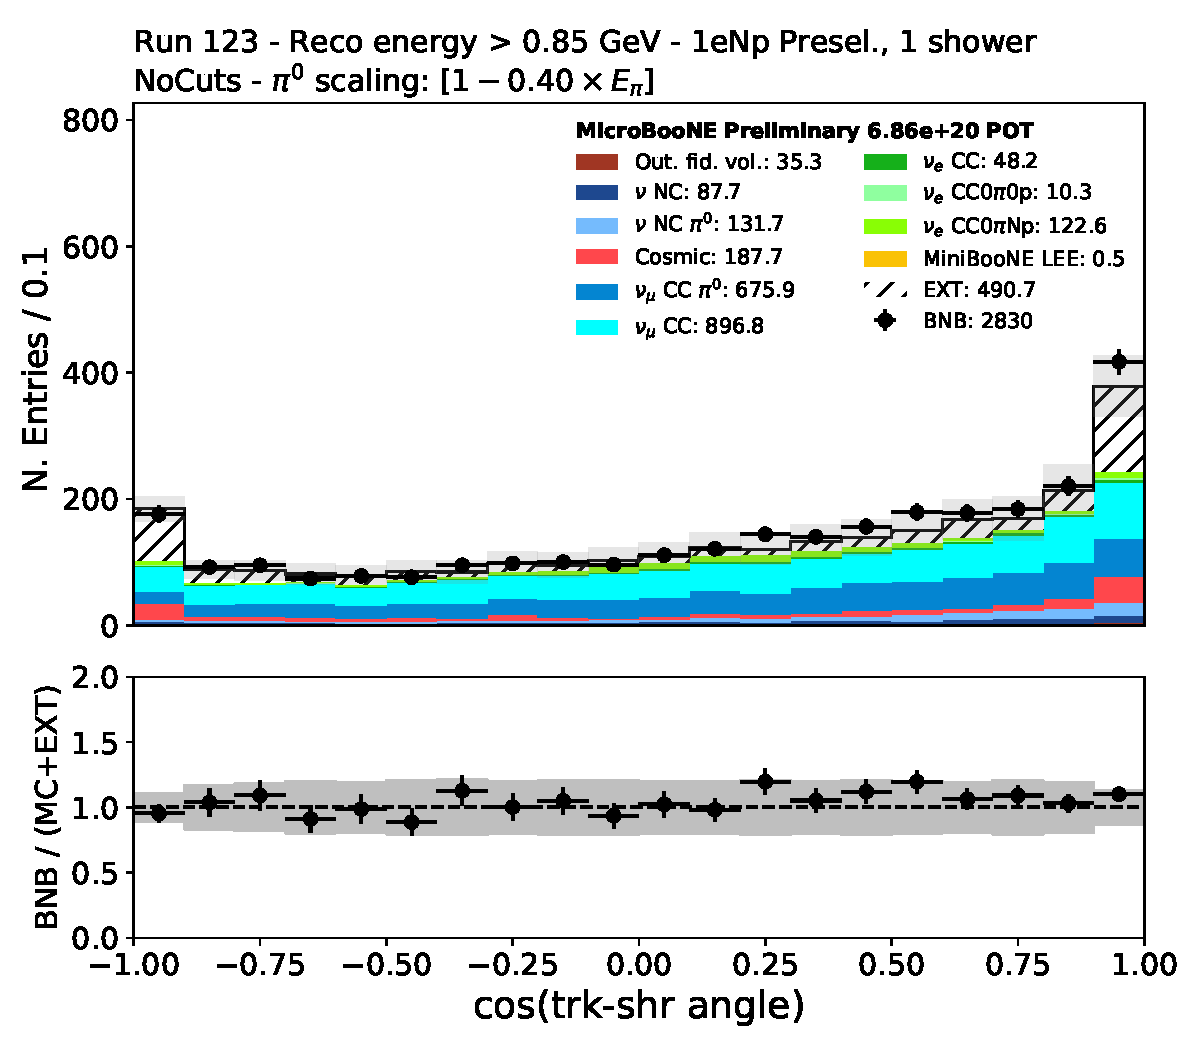
\includegraphics[width=1.0\textwidth]{Sidebands/Figures/1eNp/HighEnergy/HiEext_NPOneShr_None_pi0e040/tksh_angle.pdf}
    \caption{tksh\_angle}
    \end{subfigure}
    \begin{subfigure}{0.3\textwidth}
    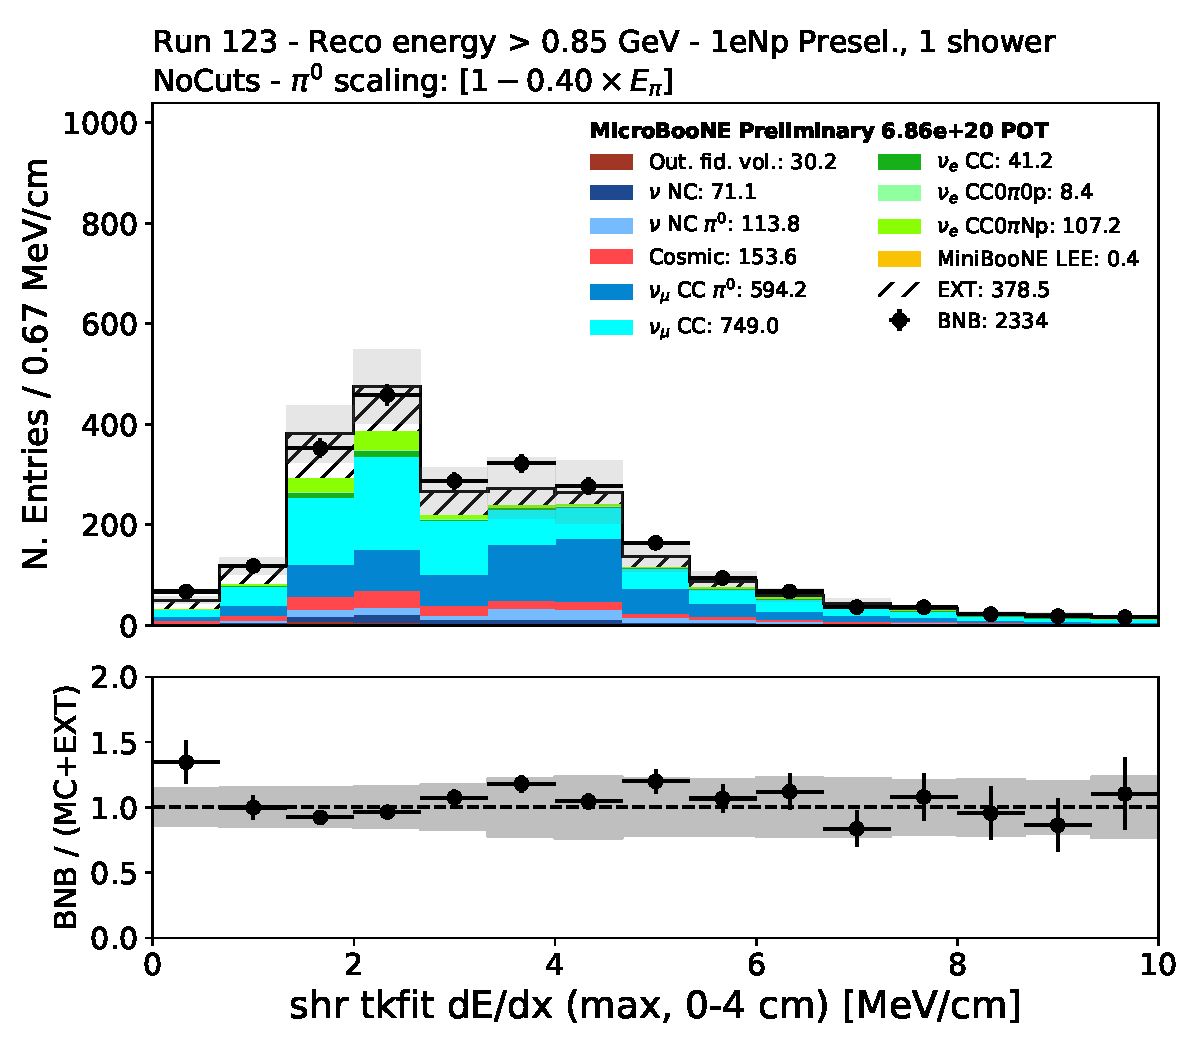
\includegraphics[width=1.0\textwidth]{Sidebands/Figures/1eNp/HighEnergy/HiEext_NPOneShr_None_pi0e040/shr_tkfit_dedx_max.pdf}
    \caption{shr\_tkfit\_dedx\_max}
    \end{subfigure}
    \caption{} 
    \label{fig:HE_1eNp_1}
\end{figure}

\begin{figure}[H]
    \centering
    \begin{subfigure}{0.3\textwidth}
    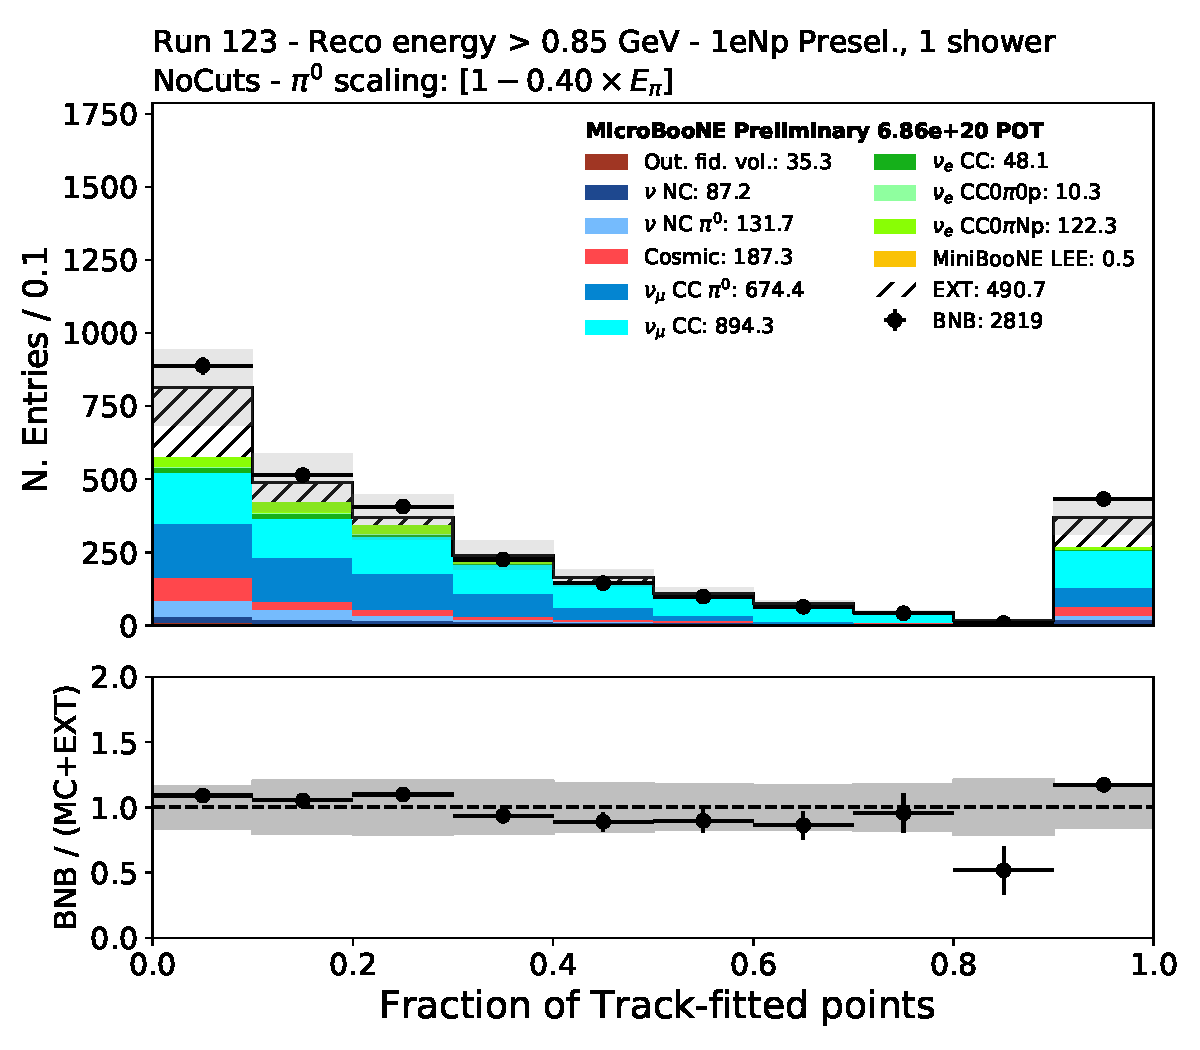
\includegraphics[width=1.0\textwidth]{Sidebands/Figures/1eNp/HighEnergy/HiEext_NPOneShr_None_pi0e040/trkfit.pdf}
    \caption{trkfit}
    \end{subfigure}
    \begin{subfigure}{0.3\textwidth}
    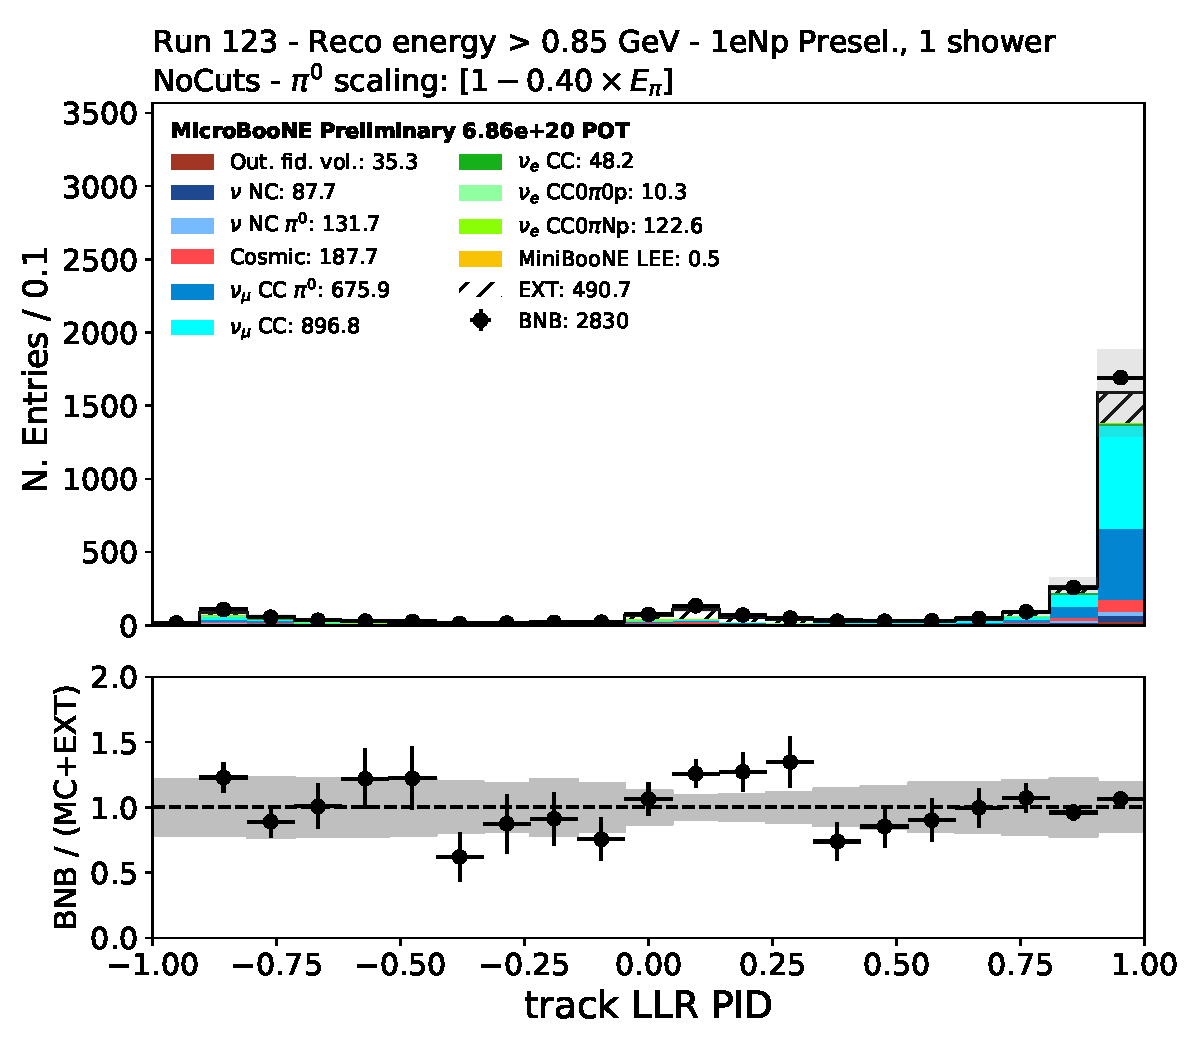
\includegraphics[width=1.0\textwidth]{Sidebands/Figures/1eNp/HighEnergy/HiEext_NPOneShr_None_pi0e040/trkpid.pdf}
    \caption{trkpid}
    \end{subfigure}
    \begin{subfigure}{0.3\textwidth}
    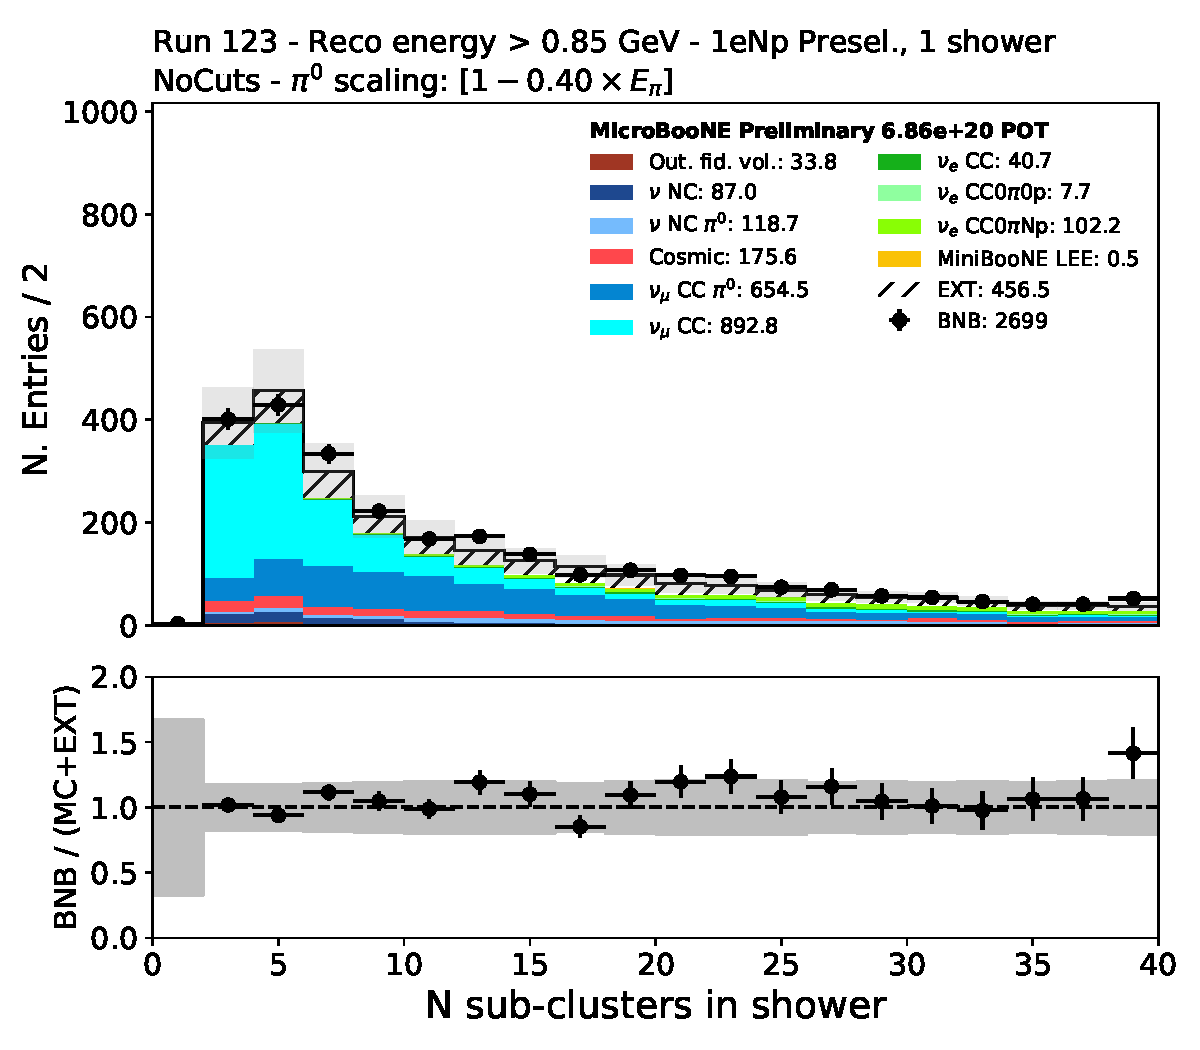
\includegraphics[width=1.0\textwidth]{Sidebands/Figures/1eNp/HighEnergy/HiEext_NPOneShr_None_pi0e040/subcluster.pdf}
    \caption{subcluster}
    \end{subfigure}
    \caption{} 
    \label{fig:HE_1eNp_2}
\end{figure}

\begin{figure}[H]
    \centering
    \begin{subfigure}{0.3\textwidth}
    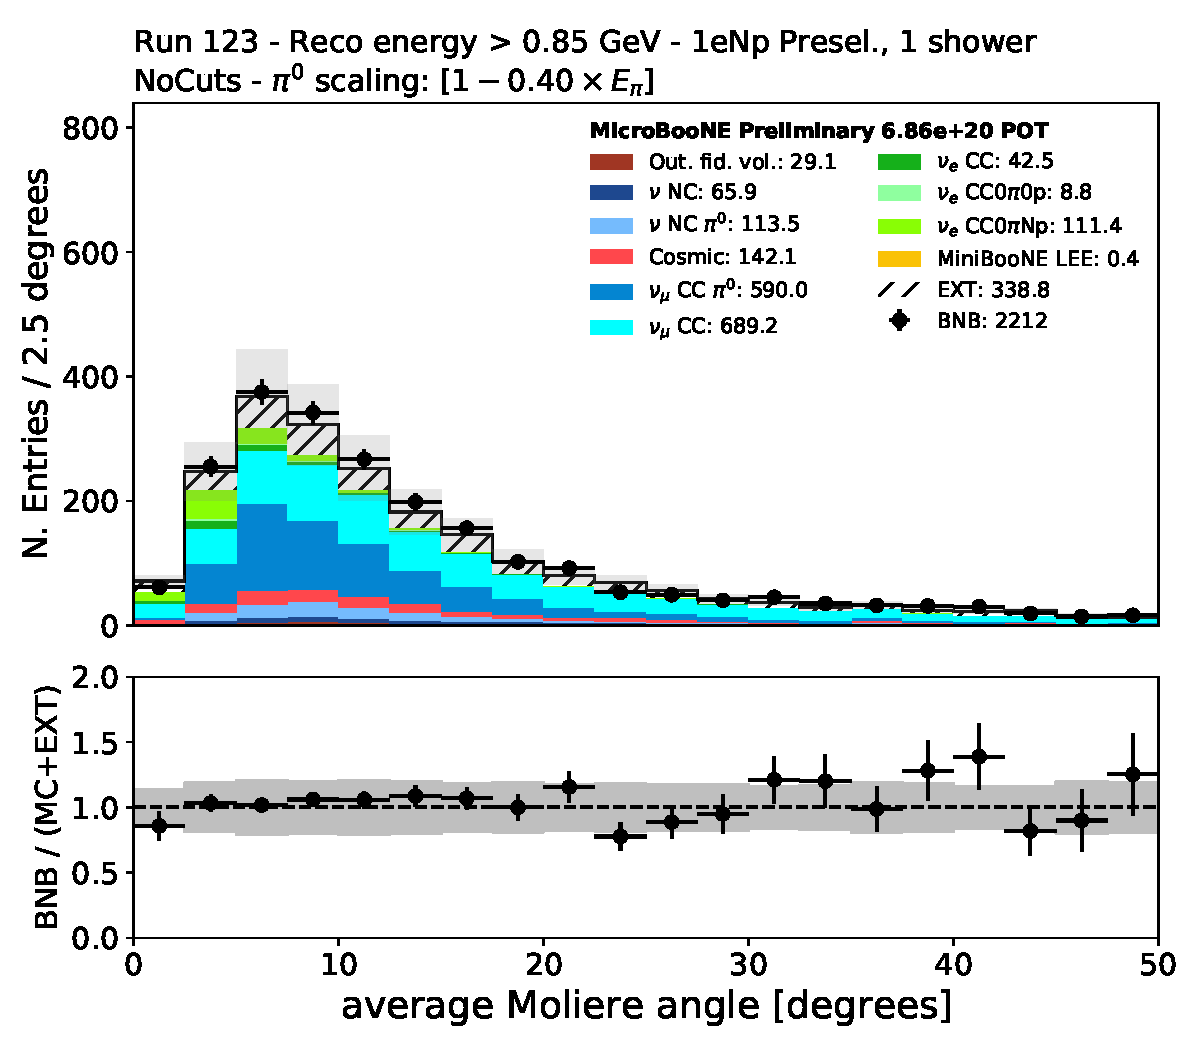
\includegraphics[width=1.0\textwidth]{Sidebands/Figures/1eNp/HighEnergy/HiEext_NPOneShr_None_pi0e040/shrmoliereavg.pdf}
    \caption{shrmoliereavg}
    \end{subfigure}
    \begin{subfigure}{0.3\textwidth}
    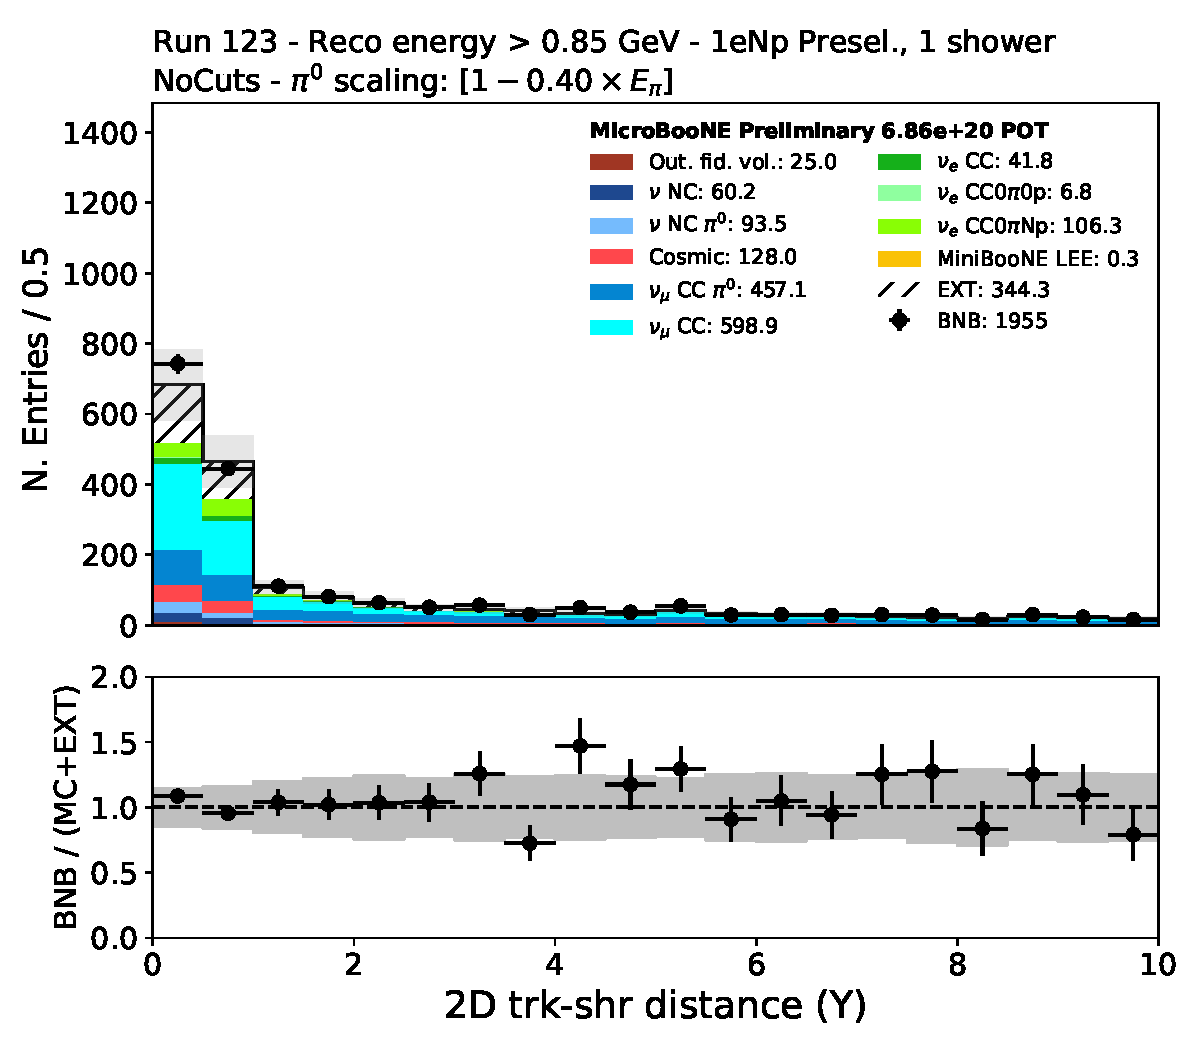
\includegraphics[width=1.0\textwidth]{Sidebands/Figures/1eNp/HighEnergy/HiEext_NPOneShr_None_pi0e040/trkshrhitdist2.pdf}
    \caption{tkshrhitdist2}
    \end{subfigure}
    \begin{subfigure}{0.3\textwidth}
    \includegraphics[width=1.0\textwidth]{Sidebands/Figures/1eNp/HighEnergy/HiEext_NPOneShr_None_pi0e040/hits_ratio.pdf}
    \caption{hits\_ratio}
    \end{subfigure}
    \caption{} 
    \label{fig:HE_1eNp_3}
\end{figure}

\begin{figure}[H]
    \centering
    \begin{subfigure}{0.3\textwidth}
    \includegraphics[width=1.0\textwidth]{Sidebands/Figures/1eNp/HighEnergy/HiEext_NPOneShr_None_pi0e040/secondshower_Y_nhit.pdf}
    \caption{secondshower\_Y\_nhit}
    \end{subfigure}
    \begin{subfigure}{0.3\textwidth}
    \includegraphics[width=1.0\textwidth]{Sidebands/Figures/1eNp/HighEnergy/HiEext_NPOneShr_None_pi0e040/secondshower_Y_vtxdist.pdf}
    \caption{secondshower\_Y\_vtxdist}
    \end{subfigure}
    \begin{subfigure}{0.3\textwidth}
    \includegraphics[width=1.0\textwidth]{Sidebands/Figures/1eNp/HighEnergy/HiEext_NPOneShr_None_pi0e040/secondshower_Y_dot.pdf}
    \caption{secondshower\_Y\_dot}
    \end{subfigure}
    \caption{} 
    \label{fig:HE_1eNp_4}
\end{figure}

\begin{figure}[H]
    \centering
    \begin{subfigure}{0.3\textwidth}
    \includegraphics[width=1.0\textwidth]{Sidebands/Figures/1eNp/HighEnergy/HiEext_NPOneShr_None_pi0e040/anglediff_Y.pdf}
    \caption{anglediff\_Y}
    \end{subfigure}
    \begin{subfigure}{0.3\textwidth}
    \includegraphics[width=1.0\textwidth]{Sidebands/Figures/1eNp/HighEnergy/HiEext_NPOneShr_None_pi0e040/CosmicIPAll3D.pdf}
    \caption{CosmicIPAll3D}
    \end{subfigure}
    \begin{subfigure}{0.3\textwidth}
    \includegraphics[width=1.0\textwidth]{Sidebands/Figures/1eNp/HighEnergy/HiEext_NPOneShr_None_pi0e040/CosmicDirAll3D.pdf}
    \caption{CosmidDirAll3D}
    \end{subfigure}
    \caption{} 
    \label{fig:HE_1eNp_5}
\end{figure}

Figures~\ref{fig:HE_1eNp_7} and~\ref{fig:HE_1eNp_8} show the BDT response from the \npsel high-energy sideband.

\begin{figure}[H]
    \centering
    \begin{subfigure}{0.4\textwidth}
    \includegraphics[width=1.0\textwidth]{Sidebands/Figures/1eNp/HighEnergy/HiEext_NPOneShr_None_pi0e040/nonpi0_score_log.pdf}
    \caption{$\pi^0$ BDT}
    \end{subfigure}
    \begin{subfigure}{0.4\textwidth}
    \includegraphics[width=1.0\textwidth]{Sidebands/Figures/1eNp/HighEnergy/HiEext_NPOneShr_None_pi0e040/nonpi0_score_high_bdt.pdf}
    \caption{$\pi^0$ BDT}
    \end{subfigure}
    \caption{} 
    \label{fig:HE_1eNp_7}
\end{figure}

\begin{figure}[H]
    \centering
    \begin{subfigure}{0.4\textwidth}
    \includegraphics[width=1.0\textwidth]{Sidebands/Figures/1eNp/HighEnergy/HiEext_NPOneShr_None_pi0e040/pi0_score_log.pdf}
    \caption{non-$\pi^0$ BDT}
    \end{subfigure}
    \begin{subfigure}{0.4\textwidth}
    \includegraphics[width=1.0\textwidth]{Sidebands/Figures/1eNp/HighEnergy/HiEext_NPOneShr_None_pi0e040/pi0_score_high_bdt.pdf}
    \caption{non-$\pi^0$ BDT}
    \end{subfigure}
    \caption{} 
    \label{fig:HE_1eNp_8}
\end{figure}

\newpage

Figures~\ref{fig:HE_1eNp_L_1} to~\ref{fig:HE_1eNp_L_5} show all BDT input variables from the HE sideband at loose selection stage.

\begin{figure}[H]
    \centering
    \begin{subfigure}{0.3\textwidth}
    \includegraphics[width=1.0\textwidth]{Sidebands/Figures/1eNp/HighEnergy/HiEext_NPOneShr_NPL_pi0e040/tksh_distance.pdf}
    \caption{tksh\_distance}
    \end{subfigure}
    \begin{subfigure}{0.3\textwidth}
    \includegraphics[width=1.0\textwidth]{Sidebands/Figures/1eNp/HighEnergy/HiEext_NPOneShr_NPL_pi0e040/tksh_angle.pdf}
    \caption{tksh\_angle}
    \end{subfigure}
    \begin{subfigure}{0.3\textwidth}
    \includegraphics[width=1.0\textwidth]{Sidebands/Figures/1eNp/HighEnergy/HiEext_NPOneShr_NPL_pi0e040/shr_tkfit_dedx_max.pdf}
    \caption{shr\_tkfit\_dedx\_max}
    \end{subfigure}
    \caption{} 
    \label{fig:HE_1eNp_L_1}
\end{figure}

\begin{figure}[H]
    \centering
    \begin{subfigure}{0.3\textwidth}
    \includegraphics[width=1.0\textwidth]{Sidebands/Figures/1eNp/HighEnergy/HiEext_NPOneShr_NPL_pi0e040/trkfit.pdf}
    \caption{trkfit}
    \end{subfigure}
    \begin{subfigure}{0.3\textwidth}
    \includegraphics[width=1.0\textwidth]{Sidebands/Figures/1eNp/HighEnergy/HiEext_NPOneShr_NPL_pi0e040/trkpid.pdf}
    \caption{trkpid}
    \end{subfigure}
    \begin{subfigure}{0.3\textwidth}
    \includegraphics[width=1.0\textwidth]{Sidebands/Figures/1eNp/HighEnergy/HiEext_NPOneShr_NPL_pi0e040/subcluster.pdf}
    \caption{subcluster}
    \end{subfigure}
    \caption{} 
    \label{fig:HE_1eNp_L_2}
\end{figure}

\begin{figure}[H]
    \centering
    \begin{subfigure}{0.3\textwidth}
    \includegraphics[width=1.0\textwidth]{Sidebands/Figures/1eNp/HighEnergy/HiEext_NPOneShr_NPL_pi0e040/shrmoliereavg.pdf}
    \caption{shrmoliereavg}
    \end{subfigure}
    \begin{subfigure}{0.3\textwidth}
    \includegraphics[width=1.0\textwidth]{Sidebands/Figures/1eNp/HighEnergy/HiEext_NPOneShr_NPL_pi0e040/trkshrhitdist2.pdf}
    \caption{tkshrhitdist2}
    \end{subfigure}
    \begin{subfigure}{0.3\textwidth}
    \includegraphics[width=1.0\textwidth]{Sidebands/Figures/1eNp/HighEnergy/HiEext_NPOneShr_NPL_pi0e040/hits_ratio.pdf}
    \caption{hits\_ratio}
    \end{subfigure}
    \caption{} 
    \label{fig:HE_1eNp_L_3}
\end{figure}

\begin{figure}[H]
    \centering
    \begin{subfigure}{0.3\textwidth}
    \includegraphics[width=1.0\textwidth]{Sidebands/Figures/1eNp/HighEnergy/HiEext_NPOneShr_NPL_pi0e040/secondshower_Y_nhit.pdf}
    \caption{secondshower\_Y\_nhit}
    \end{subfigure}
    \begin{subfigure}{0.3\textwidth}
    \includegraphics[width=1.0\textwidth]{Sidebands/Figures/1eNp/HighEnergy/HiEext_NPOneShr_NPL_pi0e040/secondshower_Y_vtxdist.pdf}
    \caption{secondshower\_Y\_vtxdist}
    \end{subfigure}
    \begin{subfigure}{0.3\textwidth}
    \includegraphics[width=1.0\textwidth]{Sidebands/Figures/1eNp/HighEnergy/HiEext_NPOneShr_NPL_pi0e040/secondshower_Y_dot.pdf}
    \caption{secondshower\_Y\_dot}
    \end{subfigure}
    \caption{} 
    \label{fig:HE_1eNp_L_4}
\end{figure}

\begin{figure}[H]
    \centering
    \begin{subfigure}{0.3\textwidth}
    \includegraphics[width=1.0\textwidth]{Sidebands/Figures/1eNp/HighEnergy/HiEext_NPOneShr_NPL_pi0e040/anglediff_Y.pdf}
    \caption{anglediff\_Y}
    \end{subfigure}
    \begin{subfigure}{0.3\textwidth}
    \includegraphics[width=1.0\textwidth]{Sidebands/Figures/1eNp/HighEnergy/HiEext_NPOneShr_NPL_pi0e040/CosmicIPAll3D.pdf}
    \caption{CosmicIPAll3D}
    \end{subfigure}
    \begin{subfigure}{0.3\textwidth}
    \includegraphics[width=1.0\textwidth]{Sidebands/Figures/1eNp/HighEnergy/HiEext_NPOneShr_NPL_pi0e040/CosmicDirAll3D.pdf}
    \caption{CosmidDirAll3D}
    \end{subfigure}
    \caption{} 
    \label{fig:HE_1eNp_L_5}
\end{figure}

\begin{table}[H]
\centering
\setlength{\tabcolsep}{10pt}
\renewcommand{\arraystretch}{1.25}
\begin{tabular}{| c | c | c | c | c | c | c | } 
 \hline
\multirow{3}{*}{variable} & \multicolumn{6}{c|}{p-values} \\
\cline{2-7} & \multicolumn{3}{c|}{pre-selection} & \multicolumn{3}{c|}{loose cuts}  \\
\cline{2-7} & stat-only & diag syst. & covariance & stat-only & diag syst. & covariance \\ \hline
n\_showers\_contained & 0.006 & 0.766 & 0.766 & 0.401 & 0.614 & 0.614 \\ \hline
n\_tracks\_contained & 0.000 & 0.934 & 0.080 & 0.038 & 0.105 & 0.074 \\ \hline
hits\_ratio & 0.003 & 0.980 & 0.089 & 0.021 & 0.094 & 0.070 \\ \hline
CosmicIPAll3D & 0.172 & 0.995 & 0.704 & 0.152 & 0.287 & 0.299 \\ \hline
CosmicDirAll3D & 0.004 & 0.995 & 0.086 & 0.683 & 0.826 & 0.820 \\ \hline
trkfit & 0.000 & 0.868 & 0.115 & 0.396 & 0.567 & 0.560 \\ \hline
shrmoliereavg & 0.367 & 0.987 & 0.756 & 0.888 & 0.949 & 0.969 \\ \hline
shr\_score & 0.112 & 0.999 & 0.857 & 0.044 & 0.084 & 0.078 \\ \hline
subcluster & 0.082 & 0.971 & 0.663 & 0.274 & 0.483 & 0.433 \\ \hline
secondshower\_Y\_nhit & 0.053 & 0.969 & 0.420 & 0.248 & 0.369 & 0.358 \\ \hline
secondshower\_Y\_dot & 0.393 & 0.993 & 0.918 & 0.928 & 0.972 & 0.975 \\ \hline
anglediff\_Y & 0.004 & 0.998 & 0.171 & 0.340 & 0.539 & 0.555 \\ \hline
secondshower\_Y\_vtxdist & 0.771 & 1.000 & 0.998 & 0.740 & 0.871 & 0.845 \\ \hline
shr\_tkfit\_dedx\_max & 0.026 & 0.984 & 0.370 & 0.454 & 0.574 & 0.555 \\ \hline
shr\_trk\_sce\_start\_y & 0.024 & 0.996 & 0.239 & 0.458 & 0.667 & 0.658 \\ \hline
shr\_trk\_sce\_end\_y & 0.013 & 0.998 & 0.268 & 0.083 & 0.215 & 0.207 \\ \hline
tksh\_angle & 0.273 & 1.000 & 0.888 & 0.996 & 0.999 & 0.999 \\ \hline
trkshrhitdist2 & 0.066 & 0.984 & 0.320 & 0.945 & 0.978 & 0.979 \\ \hline
tksh\_distance & 0.002 & 0.882 & 0.109 & 0.424 & 0.623 & 0.571 \\ \hline
trkpid & 0.000 & 0.004 & 0.000 & 0.854 & 0.920 & 0.912 \\ \hline
nonpi0\_score & 0.017 & 0.561 & 0.268 & 0.000 & 0.006 & 0.003 \\ \hline
pi0\_score & 0.011 & 0.593 & 0.240 & 0.016 & 0.105 & 0.080 \\ \hline
reco\_e & 0.084 & 0.990 & 0.466 & 0.337 & 0.516 & 0.475 \\ \hline
 \end{tabular}
 \caption{\label{tab:HiENPpvalues}p-values from the high-energy \npsel sideband for input variables to the \npsel in addition to the final BDT scores (\texttt{pi0\_score}, \texttt{nonpi0\_score}) and the reconstructed energy spectrum \texttt{reco\_e}. The three columns show the p-values computed through statistics-only uncertainties (left), with systematics but not accounting for correlations in systematics (center), and finally including the full systematics covariance matrix. Systematics include flux, cross-sections, and re-interaction uncertainties, but not detector uncertainties.}
\end{table}

Figures~\ref{fig:HE_1eNp_9} and~\ref{fig:HE_1eNp_10} show select kinematics distributions for selected \npsel events.

\begin{figure}[H]
    \centering
    \begin{subfigure}{0.3\textwidth}
    \includegraphics[width=1.0\textwidth]{Sidebands/Figures/1eNp/HighEnergy/HiEext_NPOneShr_NPBDT_pi0e040/n_tracks_contained.pdf}
    \caption{}
    \end{subfigure}
    \begin{subfigure}{0.3\textwidth}
    \includegraphics[width=1.0\textwidth]{Sidebands/Figures/1eNp/HighEnergy/HiEext_NPOneShr_NPBDT_pi0e040/protonenergy.pdf}
    \caption{}
    \end{subfigure}
    \begin{subfigure}{0.3\textwidth}
    \includegraphics[width=1.0\textwidth]{Sidebands/Figures/1eNp/HighEnergy/HiEext_NPOneShr_NPBDT_pi0e040/trk_theta.pdf}
    \caption{}
    \end{subfigure}
    \caption{} 
    \label{fig:HE_1eNp_9}
\end{figure}

\begin{figure}[H]
    \centering
    \begin{subfigure}{0.3\textwidth}
    \includegraphics[width=1.0\textwidth]{Sidebands/Figures/1eNp/HighEnergy/HiEext_NPOneShr_NPBDT_pi0e040/shr_theta.pdf}
    \caption{}
    \end{subfigure}
    \begin{subfigure}{0.3\textwidth}
    \includegraphics[width=1.0\textwidth]{Sidebands/Figures/1eNp/HighEnergy/HiEext_NPOneShr_NPBDT_pi0e040/pt.pdf}
    \caption{}
    \end{subfigure}
    \begin{subfigure}{0.3\textwidth}
    \includegraphics[width=1.0\textwidth]{Sidebands/Figures/1eNp/HighEnergy/HiEext_NPOneShr_NPBDT_pi0e040/shr_phi.pdf}
    \caption{}
    \end{subfigure}
    \caption{} 
    \label{fig:HE_1eNp_10}
\end{figure}

\subsection{\zpsel 2+ shower Sideband}
\subsubsection{\zpsel Preselection}
\begin{figure}[H]
    \centering
    \begin{subfigure}{0.3\textwidth}
    \includegraphics[width=1.0\textwidth]{Sidebands/Figures/TwoShr_1e0pSel/Presel/anglediff_U.pdf}
    \caption{angle diff U}
    \end{subfigure}
    \begin{subfigure}{0.3\textwidth}
    \includegraphics[width=1.0\textwidth]{Sidebands/Figures/TwoShr_1e0pSel/Presel/anglediff_V.pdf}
    \caption{angle diff V}
    \end{subfigure}
    \begin{subfigure}{0.3\textwidth}
    \includegraphics[width=1.0\textwidth]{Sidebands/Figures/TwoShr_1e0pSel/Presel/anglediff_Y.pdf}
    \caption{angle diff Y}
    \end{subfigure}
    \caption{} 
    \label{fig:HE_1eNp_1}
\end{figure}

\begin{figure}[H]
    \centering
    \begin{subfigure}{0.3\textwidth}
    \includegraphics[width=1.0\textwidth]{Sidebands/Figures/TwoShr_1e0pSel/Presel/CosmicDirAll3D.pdf}
    \caption{cosmic dir all 3D}
    \end{subfigure}
    \begin{subfigure}{0.3\textwidth}
    \includegraphics[width=1.0\textwidth]{Sidebands/Figures/TwoShr_1e0pSel/Presel/CosmicIPAll3D.pdf}
    \caption{cosmic IP all 3D}
    \end{subfigure}
    \begin{subfigure}{0.3\textwidth}
    \includegraphics[width=1.0\textwidth]{Sidebands/Figures/TwoShr_1e0pSel/Presel/CylFrac2h_1cm.pdf}
    \caption{CylFrac2h 1cm}
    \end{subfigure}
    \caption{} 
    \label{fig:HE_1eNp_1}
\end{figure}

\begin{figure}[H]
    \centering
    \begin{subfigure}{0.3\textwidth}
    \includegraphics[width=1.0\textwidth]{Sidebands/Figures/TwoShr_1e0pSel/Presel/DeltaRMS2h.pdf}
    \caption{delta rms 2h}
    \end{subfigure}
    \begin{subfigure}{0.3\textwidth}
    \includegraphics[width=1.0\textwidth]{Sidebands/Figures/TwoShr_1e0pSel/Presel/shr_trk_len.pdf}
    \caption{shr trk len}
    \end{subfigure}
    \begin{subfigure}{0.3\textwidth}
    \includegraphics[width=1.0\textwidth]{Sidebands/Figures/TwoShr_1e0pSel/Presel/n_showers_contained.pdf}
    \caption{n showers contained}
    \end{subfigure}
    \caption{} 
    \label{fig:HE_1eNp_1}
\end{figure}

\begin{figure}[H]
    \centering
    \begin{subfigure}{0.3\textwidth}
    \includegraphics[width=1.0\textwidth]{Sidebands/Figures/TwoShr_1e0pSel/Presel/reco_nu_vtx_x.pdf}
    \caption{x vertex}
    \end{subfigure}
    \begin{subfigure}{0.3\textwidth}
    \includegraphics[width=1.0\textwidth]{Sidebands/Figures/TwoShr_1e0pSel/Presel/reco_nu_vtx_y.pdf}
    \caption{y vertex}
    \end{subfigure}
    \begin{subfigure}{0.3\textwidth}
    \includegraphics[width=1.0\textwidth]{Sidebands/Figures/TwoShr_1e0pSel/Presel/reco_nu_vtx_z.pdf}
    \caption{z vertex}
    \end{subfigure}
    \caption{} 
    \label{fig:HE_1eNp_1}
\end{figure}

\begin{figure}[H]
    \centering
    \begin{subfigure}{0.3\textwidth}
    \includegraphics[width=1.0\textwidth]{Sidebands/Figures/TwoShr_1e0pSel/Presel/secondshower_U_dot.pdf}
    \caption{second shower dot U}
    \end{subfigure}
    \begin{subfigure}{0.3\textwidth}
    \includegraphics[width=1.0\textwidth]{Sidebands/Figures/TwoShr_1e0pSel/Presel/secondshower_V_dot.pdf}
    \caption{second shower dot V}
    \end{subfigure}
    \begin{subfigure}{0.3\textwidth}
    \includegraphics[width=1.0\textwidth]{Sidebands/Figures/TwoShr_1e0pSel/Presel/secondshower_Y_dot.pdf}
    \caption{second shower dot Y}
    \end{subfigure}
    \caption{} 
    \label{fig:HE_1eNp_1}
\end{figure}

\begin{figure}[H]
    \centering
    \begin{subfigure}{0.3\textwidth}
    \includegraphics[width=1.0\textwidth]{Sidebands/Figures/TwoShr_1e0pSel/Presel/secondshower_U_nhit.pdf}
    \caption{second shower nhit U}
    \end{subfigure}
    \begin{subfigure}{0.3\textwidth}
    \includegraphics[width=1.0\textwidth]{Sidebands/Figures/TwoShr_1e0pSel/Presel/secondshower_V_nhit.pdf}
    \caption{second shower nhit V}
    \end{subfigure}
    \begin{subfigure}{0.3\textwidth}
    \includegraphics[width=1.0\textwidth]{Sidebands/Figures/TwoShr_1e0pSel/Presel/secondshower_Y_nhit.pdf}
    \caption{second shower nhit Y}
    \end{subfigure}
    \caption{} 
    \label{fig:HE_1eNp_1}
\end{figure}

\begin{figure}[H]
    \centering
    \begin{subfigure}{0.3\textwidth}
    \includegraphics[width=1.0\textwidth]{Sidebands/Figures/TwoShr_1e0pSel/Presel/secondshower_U_vtxdist.pdf}
    \caption{second shower vtxdist U}
    \end{subfigure}
    \begin{subfigure}{0.3\textwidth}
    \includegraphics[width=1.0\textwidth]{Sidebands/Figures/TwoShr_1e0pSel/Presel/secondshower_V_vtxdist.pdf}
    \caption{second shower vtxdist V}
    \end{subfigure}
    \begin{subfigure}{0.3\textwidth}
    \includegraphics[width=1.0\textwidth]{Sidebands/Figures/TwoShr_1e0pSel/Presel/secondshower_Y_vtxdist.pdf}
    \caption{second shower vtxdist Y}
    \end{subfigure}
    \caption{} 
    \label{fig:HE_1eNp_1}
\end{figure}

\begin{figure}[H]
    \centering
    \begin{subfigure}{0.3\textwidth}
    \includegraphics[width=1.0\textwidth]{Sidebands/Figures/TwoShr_1e0pSel/Presel/shr_tkfit_2cm_dedx_U.pdf}
    \caption{shr tkfit 2cm dedx U}
    \end{subfigure}
    \begin{subfigure}{0.3\textwidth}
    \includegraphics[width=1.0\textwidth]{Sidebands/Figures/TwoShr_1e0pSel/Presel/shr_tkfit_2cm_dedx_V.pdf}
    \caption{shr tkfit 2cm dedx V}
    \end{subfigure}
    \begin{subfigure}{0.3\textwidth}
    \includegraphics[width=1.0\textwidth]{Sidebands/Figures/TwoShr_1e0pSel/Presel/shr_tkfit_2cm_dedx_V.pdf}
    \caption{shr tkfit 2cm dedx Y}
    \end{subfigure}
    \caption{} 
    \label{fig:HE_1eNp_1}
\end{figure}

\begin{figure}[H]
    \centering
    \begin{subfigure}{0.3\textwidth}
    \includegraphics[width=1.0\textwidth]{Sidebands/Figures/TwoShr_1e0pSel/Presel/shr_tkfit_gap10_dedx_U.pdf}
    \caption{shr tkfit gap10 dedx U}
    \end{subfigure}
    \begin{subfigure}{0.3\textwidth}
    \includegraphics[width=1.0\textwidth]{Sidebands/Figures/TwoShr_1e0pSel/Presel/shr_tkfit_gap10_dedx_V.pdf}
    \caption{shr tkfit gap10 dedx V}
    \end{subfigure}
    \begin{subfigure}{0.3\textwidth}
    \includegraphics[width=1.0\textwidth]{Sidebands/Figures/TwoShr_1e0pSel/Presel/shr_tkfit_gap10_dedx_V.pdf}
    \caption{shr tkfit gap10 dedx Y}
    \end{subfigure}
    \caption{} 
    \label{fig:HE_1eNp_1}
\end{figure}

\begin{figure}[H]
    \centering
    \begin{subfigure}{0.3\textwidth}
    \includegraphics[width=1.0\textwidth]{Sidebands/Figures/TwoShr_1e0pSel/Presel/shr_trk_sce_end_y.pdf}
    \caption{shr tkfit end y}
    \end{subfigure}
    \begin{subfigure}{0.3\textwidth}
    \includegraphics[width=1.0\textwidth]{Sidebands/Figures/TwoShr_1e0pSel/Presel/shr_trk_sce_start_y.pdf}
    \caption{shr tkfit start y}
    \end{subfigure}
    \begin{subfigure}{0.3\textwidth}
    \includegraphics[width=1.0\textwidth]{Sidebands/Figures/TwoShr_1e0pSel/Presel/shrMCSMom.pdf}
    \caption{shr mcs mom}
    \end{subfigure}
    \caption{} 
    \label{fig:HE_1eNp_1}
\end{figure}

\begin{figure}[H]
    \centering
    \begin{subfigure}{0.3\textwidth}
    \includegraphics[width=1.0\textwidth]{Sidebands/Figures/TwoShr_1e0pSel/Presel/shrmoliereavg.pdf}
    \caption{shr moliere avg}
    \end{subfigure}
    \begin{subfigure}{0.3\textwidth}
    \includegraphics[width=1.0\textwidth]{Sidebands/Figures/TwoShr_1e0pSel/Presel/shrPCA1CMed_5cm.pdf}
    \caption{shr pca med 5cm}
    \end{subfigure}
    \begin{subfigure}{0.3\textwidth}
    \includegraphics[width=1.0\textwidth]{Sidebands/Figures/TwoShr_1e0pSel/Presel/subcluster.pdf}
    \caption{subcluster}
    \end{subfigure}
    \caption{} 
    \label{fig:HE_1eNp_1}
\end{figure}

Table~\ref{tab:1e0p:twopshr:pvalues} collects the p-values for variables used in the \zpsel at pre-selection from the 2+ shower sideband.

\begin{table}[H]
\centering
\setlength{\tabcolsep}{10pt}
\renewcommand{\arraystretch}{1.25}
\begin{tabular}{| c | c | c | c | } 
 \hline
\multirow{2}{*}{variable} & \multicolumn{3}{c|}{p-values} \\
\cline{2-4} & stat-only & diag syst. & full covariance \\ \hline
hits\_ratio & 0.255 & 0.849 & 0.849 \\ \hline
CosmicIPAll3D & 0.000 & 0.633 & 0.014 \\ \hline
CosmicDirAll3D & 0.000 & 0.833 & 0.034 \\ \hline
tk1sh1\_angle\_alltk & 0.392 & 0.647 & 0.579 \\ \hline
trkfit & 0.008 & 0.838 & 0.055 \\ \hline
shrmoliereavg & 0.006 & 0.319 & 0.092 \\ \hline
shr\_score & 0.129 & 0.994 & 0.976 \\ \hline
subcluster & 0.026 & 0.777 & 0.114 \\ \hline
secondshower\_Y\_nhit & 0.004 & 0.713 & 0.126 \\ \hline
secondshower\_Y\_dot & 0.031 & 0.530 & 0.251 \\ \hline
anglediff\_Y & 0.202 & 0.979 & 0.606 \\ \hline
secondshower\_Y\_vtxdist & 0.307 & 0.971 & 0.666 \\ \hline
secondshower\_V\_nhit & 0.037 & 0.834 & 0.319 \\ \hline
secondshower\_V\_dot & 0.573 & 0.993 & 0.935 \\ \hline
anglediff\_V & 0.000 & 0.006 & 0.000 \\ \hline
secondshower\_V\_vtxdist & 0.001 & 0.841 & 0.099 \\ \hline
secondshower\_U\_nhit & 0.454 & 0.992 & 0.819 \\ \hline
secondshower\_U\_dot & 0.582 & 0.984 & 0.854 \\ \hline
anglediff\_U & 0.000 & 0.011 & 0.000 \\ \hline
secondshower\_U\_vtxdist & 0.331 & 0.977 & 0.720 \\ \hline
shr\_tkfit\_dedx\_max & 0.046 & 0.906 & 0.173 \\ \hline
shr\_trk\_sce\_start\_y & 0.116 & 0.946 & 0.653 \\ \hline
shr\_trk\_sce\_end\_y & 0.000 & 0.768 & 0.193 \\ \hline
shr\_trk\_len & 0.000 & 0.000 & 0.000 \\ \hline
shr\_tkfit\_2cm\_dedx\_Y & 0.775 & 0.994 & 0.909 \\ \hline
shr\_tkfit\_2cm\_dedx\_V & 0.006 & 0.898 & 0.206 \\ \hline
shr\_tkfit\_2cm\_dedx\_U & 0.035 & 0.792 & 0.132 \\ \hline
shr\_tkfit\_gap10\_dedx\_Y & 0.012 & 0.616 & 0.142 \\ \hline
shr\_tkfit\_gap10\_dedx\_V & 0.211 & 0.855 & 0.525 \\ \hline
shr\_tkfit\_gap10\_dedx\_U & 0.199 & 0.770 & 0.380 \\ \hline
bkg\_score & 0.019 & 0.844 & 0.114 \\ \hline
 \end{tabular}
 \caption{\label{tab:1e0p:twopshr:pvalues}p-values from the 2+ shower \zpsel sideband for input variables to the \zpsel in addition to the final BDT scores (\texttt{pi0\_score}, \texttt{nonpi0\_score}) and the reconstructed energy spectrum \texttt{reco\_e}. The three columns show the p-values computed through statistics-only uncertainties (left), with systematics but not accounting for correlations in systematics (center), and finally including the full systematics covariance matrix. Systematics include flux, cross-sections, and re-interaction uncertainties, but not detector uncertainties.}
\end{table}



\subsubsection{\zpsel Loose Selection}
\begin{figure}[H]
    \centering
    \begin{subfigure}{0.3\textwidth}
    \includegraphics[width=1.0\textwidth]{Sidebands/Figures/TwoShr_1e0pSel/loose/anglediff_U.pdf}
    \caption{angle diff U}
    \end{subfigure}
    \begin{subfigure}{0.3\textwidth}
    \includegraphics[width=1.0\textwidth]{Sidebands/Figures/TwoShr_1e0pSel/loose/anglediff_V.pdf}
    \caption{angle diff V}
    \end{subfigure}
    \begin{subfigure}{0.3\textwidth}
    \includegraphics[width=1.0\textwidth]{Sidebands/Figures/TwoShr_1e0pSel/loose/anglediff_Y.pdf}
    \caption{angle diff Y}
    \end{subfigure}
    \caption{} 
    \label{fig:HE_1eNp_1}
\end{figure}

\begin{figure}[H]
    \centering
    \begin{subfigure}{0.3\textwidth}
    \includegraphics[width=1.0\textwidth]{Sidebands/Figures/TwoShr_1e0pSel/loose/CosmicDirAll3D.pdf}
    \caption{cosmic dir all 3D}
    \end{subfigure}
    \begin{subfigure}{0.3\textwidth}
    \includegraphics[width=1.0\textwidth]{Sidebands/Figures/TwoShr_1e0pSel/loose/CosmicIPAll3D.pdf}
    \caption{cosmic IP all 3D}
    \end{subfigure}
    \begin{subfigure}{0.3\textwidth}
    \includegraphics[width=1.0\textwidth]{Sidebands/Figures/TwoShr_1e0pSel/loose/CylFrac2h_1cm.pdf}
    \caption{CylFrac2h 1cm}
    \end{subfigure}
    \caption{} 
    \label{fig:HE_1eNp_1}
\end{figure}

\begin{figure}[H]
    \centering
    \begin{subfigure}{0.3\textwidth}
    \includegraphics[width=1.0\textwidth]{Sidebands/Figures/TwoShr_1e0pSel/loose/DeltaRMS2h.pdf}
    \caption{delta rms 2h}
    \end{subfigure}
    \begin{subfigure}{0.3\textwidth}
    \includegraphics[width=1.0\textwidth]{Sidebands/Figures/TwoShr_1e0pSel/loose/shr_trk_len.pdf}
    \caption{shr trk len}
    \end{subfigure}
    \begin{subfigure}{0.3\textwidth}
    \includegraphics[width=1.0\textwidth]{Sidebands/Figures/TwoShr_1e0pSel/loose/n_showers_contained.pdf}
    \caption{n showers contained}
    \end{subfigure}
    \caption{} 
    \label{fig:HE_1eNp_1}
\end{figure}

\begin{figure}[H]
    \centering
    \begin{subfigure}{0.3\textwidth}
    \includegraphics[width=1.0\textwidth]{Sidebands/Figures/TwoShr_1e0pSel/loose/reco_nu_vtx_x.pdf}
    \caption{x vertex}
    \end{subfigure}
    \begin{subfigure}{0.3\textwidth}
    \includegraphics[width=1.0\textwidth]{Sidebands/Figures/TwoShr_1e0pSel/loose/reco_nu_vtx_y.pdf}
    \caption{y vertex}
    \end{subfigure}
    \begin{subfigure}{0.3\textwidth}
    \includegraphics[width=1.0\textwidth]{Sidebands/Figures/TwoShr_1e0pSel/loose/reco_nu_vtx_z.pdf}
    \caption{z vertex}
    \end{subfigure}
    \caption{} 
    \label{fig:HE_1eNp_1}
\end{figure}

\begin{figure}[H]
    \centering
    \begin{subfigure}{0.3\textwidth}
    \includegraphics[width=1.0\textwidth]{Sidebands/Figures/TwoShr_1e0pSel/loose/secondshower_U_dot.pdf}
    \caption{second shower dot U}
    \end{subfigure}
    \begin{subfigure}{0.3\textwidth}
    \includegraphics[width=1.0\textwidth]{Sidebands/Figures/TwoShr_1e0pSel/loose/secondshower_V_dot.pdf}
    \caption{second shower dot V}
    \end{subfigure}
    \begin{subfigure}{0.3\textwidth}
    \includegraphics[width=1.0\textwidth]{Sidebands/Figures/TwoShr_1e0pSel/loose/secondshower_Y_dot.pdf}
    \caption{second shower dot Y}
    \end{subfigure}
    \caption{} 
    \label{fig:HE_1eNp_1}
\end{figure}

\begin{figure}[H]
    \centering
    \begin{subfigure}{0.3\textwidth}
    \includegraphics[width=1.0\textwidth]{Sidebands/Figures/TwoShr_1e0pSel/loose/secondshower_U_nhit.pdf}
    \caption{second shower nhit U}
    \end{subfigure}
    \begin{subfigure}{0.3\textwidth}
    \includegraphics[width=1.0\textwidth]{Sidebands/Figures/TwoShr_1e0pSel/loose/secondshower_V_nhit.pdf}
    \caption{second shower nhit V}
    \end{subfigure}
    \begin{subfigure}{0.3\textwidth}
    \includegraphics[width=1.0\textwidth]{Sidebands/Figures/TwoShr_1e0pSel/loose/secondshower_Y_nhit.pdf}
    \caption{second shower nhit Y}
    \end{subfigure}
    \caption{} 
    \label{fig:HE_1eNp_1}
\end{figure}

\begin{figure}[H]
    \centering
    \begin{subfigure}{0.3\textwidth}
    \includegraphics[width=1.0\textwidth]{Sidebands/Figures/TwoShr_1e0pSel/loose/secondshower_U_vtxdist.pdf}
    \caption{second shower vtxdist U}
    \end{subfigure}
    \begin{subfigure}{0.3\textwidth}
    \includegraphics[width=1.0\textwidth]{Sidebands/Figures/TwoShr_1e0pSel/loose/secondshower_V_vtxdist.pdf}
    \caption{second shower vtxdist V}
    \end{subfigure}
    \begin{subfigure}{0.3\textwidth}
    \includegraphics[width=1.0\textwidth]{Sidebands/Figures/TwoShr_1e0pSel/loose/secondshower_Y_vtxdist.pdf}
    \caption{second shower vtxdist Y}
    \end{subfigure}
    \caption{} 
    \label{fig:HE_1eNp_1}
\end{figure}

\begin{figure}[H]
    \centering
    \begin{subfigure}{0.3\textwidth}
    \includegraphics[width=1.0\textwidth]{Sidebands/Figures/TwoShr_1e0pSel/loose/shr_tkfit_2cm_dedx_U.pdf}
    \caption{shr tkfit 2cm dedx U}
    \end{subfigure}
    \begin{subfigure}{0.3\textwidth}
    \includegraphics[width=1.0\textwidth]{Sidebands/Figures/TwoShr_1e0pSel/loose/shr_tkfit_2cm_dedx_V.pdf}
    \caption{shr tkfit 2cm dedx V}
    \end{subfigure}
    \begin{subfigure}{0.3\textwidth}
    \includegraphics[width=1.0\textwidth]{Sidebands/Figures/TwoShr_1e0pSel/loose/shr_tkfit_2cm_dedx_V.pdf}
    \caption{shr tkfit 2cm dedx Y}
    \end{subfigure}
    \caption{} 
    \label{fig:HE_1eNp_1}
\end{figure}

\begin{figure}[H]
    \centering
    \begin{subfigure}{0.3\textwidth}
    \includegraphics[width=1.0\textwidth]{Sidebands/Figures/TwoShr_1e0pSel/loose/shr_tkfit_gap10_dedx_U.pdf}
    \caption{shr tkfit gap10 dedx U}
    \end{subfigure}
    \begin{subfigure}{0.3\textwidth}
    \includegraphics[width=1.0\textwidth]{Sidebands/Figures/TwoShr_1e0pSel/loose/shr_tkfit_gap10_dedx_V.pdf}
    \caption{shr tkfit gap10 dedx V}
    \end{subfigure}
    \begin{subfigure}{0.3\textwidth}
    \includegraphics[width=1.0\textwidth]{Sidebands/Figures/TwoShr_1e0pSel/loose/shr_tkfit_gap10_dedx_V.pdf}
    \caption{shr tkfit gap10 dedx Y}
    \end{subfigure}
    \caption{} 
    \label{fig:HE_1eNp_1}
\end{figure}

\begin{figure}[H]
    \centering
    \begin{subfigure}{0.3\textwidth}
    \includegraphics[width=1.0\textwidth]{Sidebands/Figures/TwoShr_1e0pSel/loose/shr_trk_sce_end_y.pdf}
    \caption{shr tkfit end y}
    \end{subfigure}
    \begin{subfigure}{0.3\textwidth}
    \includegraphics[width=1.0\textwidth]{Sidebands/Figures/TwoShr_1e0pSel/loose/shr_trk_sce_start_y.pdf}
    \caption{shr tkfit start y}
    \end{subfigure}
    \begin{subfigure}{0.3\textwidth}
    \includegraphics[width=1.0\textwidth]{Sidebands/Figures/TwoShr_1e0pSel/loose/shrMCSMom.pdf}
    \caption{shr mcs mom}
    \end{subfigure}
    \caption{} 
    \label{fig:HE_1eNp_1}
\end{figure}

\begin{figure}[H]
    \centering
    \begin{subfigure}{0.3\textwidth}
    \includegraphics[width=1.0\textwidth]{Sidebands/Figures/TwoShr_1e0pSel/loose/shrmoliereavg.pdf}
    \caption{shr moliere avg}
    \end{subfigure}
    \begin{subfigure}{0.3\textwidth}
    \includegraphics[width=1.0\textwidth]{Sidebands/Figures/TwoShr_1e0pSel/loose/shrPCA1CMed_5cm.pdf}
    \caption{shr pca med 5cm}
    \end{subfigure}
    \begin{subfigure}{0.3\textwidth}
    \includegraphics[width=1.0\textwidth]{Sidebands/Figures/TwoShr_1e0pSel/loose/subcluster.pdf}
    \caption{subcluster}
    \end{subfigure}
    \caption{} 
    \label{fig:HE_1eNp_1}
\end{figure}

\subsubsection{\zpsel BDT Selection}
\begin{figure}[H]
    \centering
    \begin{subfigure}{0.3\textwidth}
    \includegraphics[width=1.0\textwidth]{Sidebands/Figures/TwoShr_1e0pSel/BDT/anglediff_U.pdf}
    \caption{angle diff U}
    \end{subfigure}
    \begin{subfigure}{0.3\textwidth}
    \includegraphics[width=1.0\textwidth]{Sidebands/Figures/TwoShr_1e0pSel/BDT/anglediff_V.pdf}
    \caption{angle diff V}
    \end{subfigure}
    \begin{subfigure}{0.3\textwidth}
    \includegraphics[width=1.0\textwidth]{Sidebands/Figures/TwoShr_1e0pSel/BDT/anglediff_Y.pdf}
    \caption{angle diff Y}
    \end{subfigure}
    \caption{} 
    \label{fig:HE_1eNp_1}
\end{figure}

\begin{figure}[H]
    \centering
    \begin{subfigure}{0.3\textwidth}
    \includegraphics[width=1.0\textwidth]{Sidebands/Figures/TwoShr_1e0pSel/BDT/CosmicDirAll3D.pdf}
    \caption{cosmic dir all 3D}
    \end{subfigure}
    \begin{subfigure}{0.3\textwidth}
    \includegraphics[width=1.0\textwidth]{Sidebands/Figures/TwoShr_1e0pSel/BDT/CosmicIPAll3D.pdf}
    \caption{cosmic IP all 3D}
    \end{subfigure}
    \begin{subfigure}{0.3\textwidth}
    \includegraphics[width=1.0\textwidth]{Sidebands/Figures/TwoShr_1e0pSel/BDT/CylFrac2h_1cm.pdf}
    \caption{CylFrac2h 1cm}
    \end{subfigure}
    \caption{} 
    \label{fig:HE_1eNp_1}
\end{figure}

\begin{figure}[H]
    \centering
    \begin{subfigure}{0.3\textwidth}
    \includegraphics[width=1.0\textwidth]{Sidebands/Figures/TwoShr_1e0pSel/BDT/DeltaRMS2h.pdf}
    \caption{delta rms 2h}
    \end{subfigure}
    \begin{subfigure}{0.3\textwidth}
    \includegraphics[width=1.0\textwidth]{Sidebands/Figures/TwoShr_1e0pSel/BDT/shr_trk_len.pdf}
    \caption{shr trk len}
    \end{subfigure}
    \begin{subfigure}{0.3\textwidth}
    \includegraphics[width=1.0\textwidth]{Sidebands/Figures/TwoShr_1e0pSel/BDT/n_showers_contained.pdf}
    \caption{n showers contained}
    \end{subfigure}
    \caption{} 
    \label{fig:HE_1eNp_1}
\end{figure}

\begin{figure}[H]
    \centering
    \begin{subfigure}{0.3\textwidth}
    \includegraphics[width=1.0\textwidth]{Sidebands/Figures/TwoShr_1e0pSel/BDT/reco_nu_vtx_x.pdf}
    \caption{x vertex}
    \end{subfigure}
    \begin{subfigure}{0.3\textwidth}
    \includegraphics[width=1.0\textwidth]{Sidebands/Figures/TwoShr_1e0pSel/BDT/reco_nu_vtx_y.pdf}
    \caption{y vertex}
    \end{subfigure}
    \begin{subfigure}{0.3\textwidth}
    \includegraphics[width=1.0\textwidth]{Sidebands/Figures/TwoShr_1e0pSel/BDT/reco_nu_vtx_z.pdf}
    \caption{z vertex}
    \end{subfigure}
    \caption{} 
    \label{fig:HE_1eNp_1}
\end{figure}

\begin{figure}[H]
    \centering
    \begin{subfigure}{0.3\textwidth}
    \includegraphics[width=1.0\textwidth]{Sidebands/Figures/TwoShr_1e0pSel/BDT/secondshower_U_dot.pdf}
    \caption{second shower dot U}
    \end{subfigure}
    \begin{subfigure}{0.3\textwidth}
    \includegraphics[width=1.0\textwidth]{Sidebands/Figures/TwoShr_1e0pSel/BDT/secondshower_V_dot.pdf}
    \caption{second shower dot V}
    \end{subfigure}
    \begin{subfigure}{0.3\textwidth}
    \includegraphics[width=1.0\textwidth]{Sidebands/Figures/TwoShr_1e0pSel/BDT/secondshower_Y_dot.pdf}
    \caption{second shower dot Y}
    \end{subfigure}
    \caption{} 
    \label{fig:HE_1eNp_1}
\end{figure}

\begin{figure}[H]
    \centering
    \begin{subfigure}{0.3\textwidth}
    \includegraphics[width=1.0\textwidth]{Sidebands/Figures/TwoShr_1e0pSel/BDT/secondshower_U_nhit.pdf}
    \caption{second shower nhit U}
    \end{subfigure}
    \begin{subfigure}{0.3\textwidth}
    \includegraphics[width=1.0\textwidth]{Sidebands/Figures/TwoShr_1e0pSel/BDT/secondshower_V_nhit.pdf}
    \caption{second shower nhit V}
    \end{subfigure}
    \begin{subfigure}{0.3\textwidth}
    \includegraphics[width=1.0\textwidth]{Sidebands/Figures/TwoShr_1e0pSel/BDT/secondshower_Y_nhit.pdf}
    \caption{second shower nhit Y}
    \end{subfigure}
    \caption{} 
    \label{fig:HE_1eNp_1}
\end{figure}

\begin{figure}[H]
    \centering
    \begin{subfigure}{0.3\textwidth}
    \includegraphics[width=1.0\textwidth]{Sidebands/Figures/TwoShr_1e0pSel/BDT/secondshower_U_vtxdist.pdf}
    \caption{second shower vtxdist U}
    \end{subfigure}
    \begin{subfigure}{0.3\textwidth}
    \includegraphics[width=1.0\textwidth]{Sidebands/Figures/TwoShr_1e0pSel/BDT/secondshower_V_vtxdist.pdf}
    \caption{second shower vtxdist V}
    \end{subfigure}
    \begin{subfigure}{0.3\textwidth}
    \includegraphics[width=1.0\textwidth]{Sidebands/Figures/TwoShr_1e0pSel/BDT/secondshower_Y_vtxdist.pdf}
    \caption{second shower vtxdist Y}
    \end{subfigure}
    \caption{} 
    \label{fig:HE_1eNp_1}
\end{figure}

\begin{figure}[H]
    \centering
    \begin{subfigure}{0.3\textwidth}
    \includegraphics[width=1.0\textwidth]{Sidebands/Figures/TwoShr_1e0pSel/BDT/shr_tkfit_2cm_dedx_U.pdf}
    \caption{shr tkfit 2cm dedx U}
    \end{subfigure}
    \begin{subfigure}{0.3\textwidth}
    \includegraphics[width=1.0\textwidth]{Sidebands/Figures/TwoShr_1e0pSel/BDT/shr_tkfit_2cm_dedx_V.pdf}
    \caption{shr tkfit 2cm dedx V}
    \end{subfigure}
    \begin{subfigure}{0.3\textwidth}
    \includegraphics[width=1.0\textwidth]{Sidebands/Figures/TwoShr_1e0pSel/BDT/shr_tkfit_2cm_dedx_V.pdf}
    \caption{shr tkfit 2cm dedx Y}
    \end{subfigure}
    \caption{} 
    \label{fig:HE_1eNp_1}
\end{figure}

\begin{figure}[H]
    \centering
    \begin{subfigure}{0.3\textwidth}
    \includegraphics[width=1.0\textwidth]{Sidebands/Figures/TwoShr_1e0pSel/BDT/shr_tkfit_gap10_dedx_U.pdf}
    \caption{shr tkfit gap10 dedx U}
    \end{subfigure}
    \begin{subfigure}{0.3\textwidth}
    \includegraphics[width=1.0\textwidth]{Sidebands/Figures/TwoShr_1e0pSel/BDT/shr_tkfit_gap10_dedx_V.pdf}
    \caption{shr tkfit gap10 dedx V}
    \end{subfigure}
    \begin{subfigure}{0.3\textwidth}
    \includegraphics[width=1.0\textwidth]{Sidebands/Figures/TwoShr_1e0pSel/BDT/shr_tkfit_gap10_dedx_V.pdf}
    \caption{shr tkfit gap10 dedx Y}
    \end{subfigure}
    \caption{} 
    \label{fig:HE_1eNp_1}
\end{figure}

\begin{figure}[H]
    \centering
    \begin{subfigure}{0.3\textwidth}
    \includegraphics[width=1.0\textwidth]{Sidebands/Figures/TwoShr_1e0pSel/BDT/shr_trk_sce_end_y.pdf}
    \caption{shr tkfit end y}
    \end{subfigure}
    \begin{subfigure}{0.3\textwidth}
    \includegraphics[width=1.0\textwidth]{Sidebands/Figures/TwoShr_1e0pSel/BDT/shr_trk_sce_start_y.pdf}
    \caption{shr tkfit start y}
    \end{subfigure}
    \begin{subfigure}{0.3\textwidth}
    \includegraphics[width=1.0\textwidth]{Sidebands/Figures/TwoShr_1e0pSel/BDT/shrMCSMom.pdf}
    \caption{shr mcs mom}
    \end{subfigure}
    \caption{} 
    \label{fig:HE_1eNp_1}
\end{figure}

\begin{figure}[H]
    \centering
    \begin{subfigure}{0.3\textwidth}
    \includegraphics[width=1.0\textwidth]{Sidebands/Figures/TwoShr_1e0pSel/BDT/shrmoliereavg.pdf}
    \caption{shr moliere avg}
    \end{subfigure}
    \begin{subfigure}{0.3\textwidth}
    \includegraphics[width=1.0\textwidth]{Sidebands/Figures/TwoShr_1e0pSel/BDT/shrPCA1CMed_5cm.pdf}
    \caption{shr pca med 5cm}
    \end{subfigure}
    \begin{subfigure}{0.3\textwidth}
    \includegraphics[width=1.0\textwidth]{Sidebands/Figures/TwoShr_1e0pSel/BDT/subcluster.pdf}
    \caption{subcluster}
    \end{subfigure}
    \caption{} 
    \label{fig:HE_1eNp_1}
\end{figure}

\subsection{\zpsel High Energy Sideband}


Table~\ref{tab:1e0p:HE:pvalues} collects the p-values for variables used in the \zpsel at pre-selection from the HE sideband.

\begin{table}[H]
\centering
\setlength{\tabcolsep}{10pt}
\renewcommand{\arraystretch}{1.25}
\begin{tabular}{| c | c | c | c | } 
 \hline
\multirow{2}{*}{variable} & \multicolumn{3}{c|}{p-values} \\
\cline{2-4} & stat-only & diag syst. & full covariance \\ \hline
hits\_ratio & 0.304 & 0.541 & 0.541 \\ \hline
CosmicIPAll3D & 0.162 & 0.488 & 0.436 \\ \hline
CosmicDirAll3D & 0.214 & 0.559 & 0.522 \\ \hline
tk1sh1\_angle\_alltk & 0.009 & 0.045 & 0.040 \\ \hline
trkfit & 0.116 & 0.368 & 0.319 \\ \hline
shrmoliereavg & 0.571 & 0.814 & 0.772 \\ \hline
shr\_score & 0.260 & 0.720 & 0.593 \\ \hline
subcluster & 0.232 & 0.646 & 0.739 \\ \hline
secondshower\_Y\_nhit & 0.000 & 0.003 & 0.002 \\ \hline
secondshower\_Y\_dot & 0.001 & 0.014 & 0.012 \\ \hline
anglediff\_Y & 0.234 & 0.448 & 0.444 \\ \hline
secondshower\_Y\_vtxdist & 0.422 & 0.673 & 0.610 \\ \hline
secondshower\_V\_nhit & 0.071 & 0.225 & 0.208 \\ \hline
secondshower\_V\_dot & 0.159 & 0.460 & 0.491 \\ \hline
anglediff\_V & 0.201 & 0.463 & 0.403 \\ \hline
secondshower\_V\_vtxdist & 0.041 & 0.234 & 0.215 \\ \hline
secondshower\_U\_nhit & 0.001 & 0.009 & 0.007 \\ \hline
secondshower\_U\_dot & 0.000 & 0.000 & 0.000 \\ \hline
anglediff\_U & 0.118 & 0.315 & 0.328 \\ \hline
secondshower\_U\_vtxdist & 0.026 & 0.202 & 0.175 \\ \hline
shr\_tkfit\_dedx\_max & 0.294 & 0.595 & 0.626 \\ \hline
shr\_trk\_sce\_start\_y & 0.278 & 0.579 & 0.572 \\ \hline
shr\_trk\_sce\_end\_y & 0.207 & 0.585 & 0.561 \\ \hline
shr\_trk\_len & 0.202 & 0.585 & 0.548 \\ \hline
shr\_tkfit\_2cm\_dedx\_Y & 0.165 & 0.365 & 0.334 \\ \hline
shr\_tkfit\_2cm\_dedx\_V & 0.002 & 0.037 & 0.012 \\ \hline
shr\_tkfit\_2cm\_dedx\_U & 0.983 & 0.995 & 0.992 \\ \hline
shr\_tkfit\_gap10\_dedx\_Y & 0.668 & 0.866 & 0.800 \\ \hline
shr\_tkfit\_gap10\_dedx\_V & 0.158 & 0.505 & 0.404 \\ \hline
shr\_tkfit\_gap10\_dedx\_U & 0.895 & 0.967 & 0.963 \\ \hline
bkg\_score & 0.770 & 0.907 & 0.892 \\ \hline
 \end{tabular}
 \caption{\label{tab:1e0p:HE:pvalues}p-values from the high-energy \zpsel sideband for input variables to the \zpsel in addition to the final BDT scores (\texttt{pi0\_score}, \texttt{nonpi0\_score}) and the reconstructed energy spectrum \texttt{reco\_e}. The three columns show the p-values computed through statistics-only uncertainties (left), with systematics but not accounting for correlations in systematics (center), and finally including the full systematics covariance matrix. Systematics include flux, cross-sections, and re-interaction uncertainties, but not detector uncertainties.}
\end{table}

\subsection{\zpsel Low-PID Sideband}


Table~\ref{tab:1e0p:LPID:pvalues} collects the p-values for variables used in the \zpsel at pre-selection from the low-PID sideband.


\begin{table}[H]
\centering
\setlength{\tabcolsep}{10pt}
\renewcommand{\arraystretch}{1.25}
\begin{tabular}{| c | c | c | c | } 
 \hline
\multirow{2}{*}{variable} & \multicolumn{3}{c|}{p-values} \\
\cline{2-4} & stat-only & diag syst. & full covariance \\ \hline
hits\_ratio & 0.776 & 0.957 & 0.957 \\ \hline
CosmicIPAll3D & 0.005 & 0.663 & 0.078 \\ \hline
CosmicDirAll3D & 0.037 & 0.915 & 0.181 \\ \hline
tk1sh1\_angle\_alltk & 0.080 & 0.301 & 0.251 \\ \hline
trkfit & 0.452 & 0.957 & 0.622 \\ \hline
shrmoliereavg & 0.203 & 0.932 & 0.454 \\ \hline
shr\_score & 0.074 & 0.854 & 0.249 \\ \hline
subcluster & 0.842 & 1.000 & 0.947 \\ \hline
secondshower\_Y\_nhit & 0.301 & 0.895 & 0.681 \\ \hline
secondshower\_Y\_dot & 0.010 & 0.178 & 0.081 \\ \hline
anglediff\_Y & 0.178 & 0.867 & 0.438 \\ \hline
secondshower\_Y\_vtxdist & 0.862 & 0.994 & 0.947 \\ \hline
secondshower\_V\_nhit & 0.081 & 0.721 & 0.367 \\ \hline
secondshower\_V\_dot & 0.020 & 0.622 & 0.289 \\ \hline
anglediff\_V & 0.348 & 0.976 & 0.579 \\ \hline
secondshower\_V\_vtxdist & 0.331 & 0.936 & 0.568 \\ \hline
secondshower\_U\_nhit & 0.123 & 0.755 & 0.547 \\ \hline
secondshower\_U\_dot & 0.780 & 0.972 & 0.898 \\ \hline
anglediff\_U & 0.024 & 0.697 & 0.086 \\ \hline
secondshower\_U\_vtxdist & 0.877 & 0.998 & 0.963 \\ \hline
shr\_tkfit\_dedx\_max & 0.624 & 0.979 & 0.795 \\ \hline
shr\_trk\_sce\_start\_y & 0.905 & 1.000 & 0.971 \\ \hline
shr\_trk\_sce\_end\_y & 0.247 & 0.978 & 0.519 \\ \hline
shr\_trk\_len & 0.086 & 0.731 & 0.293 \\ \hline
shr\_tkfit\_2cm\_dedx\_Y & 0.437 & 0.984 & 0.762 \\ \hline
shr\_tkfit\_2cm\_dedx\_V & 0.308 & 0.959 & 0.537 \\ \hline
shr\_tkfit\_2cm\_dedx\_U & 0.766 & 0.996 & 0.891 \\ \hline
shr\_tkfit\_gap10\_dedx\_Y & 0.738 & 0.994 & 0.928 \\ \hline
shr\_tkfit\_gap10\_dedx\_V & 0.181 & 0.962 & 0.425 \\ \hline
shr\_tkfit\_gap10\_dedx\_U & 0.714 & 0.985 & 0.929 \\ \hline
bkg\_score & 0.490 & 0.960 & 0.627 \\ \hline
 \end{tabular}
 \caption{\label{tab:1e0p:LPID:pvalues}p-values from the low-pid \zpsel sideband for input variables to the \zpsel in addition to the final BDT scores (\texttt{pi0\_score}, \texttt{nonpi0\_score}) and the reconstructed energy spectrum \texttt{reco\_e}. The three columns show the p-values computed through statistics-only uncertainties (left), with systematics but not accounting for correlations in systematics (center), and finally including the full systematics covariance matrix. Systematics include flux, cross-sections, and re-interaction uncertainties, but not detector uncertainties.}
\end{table}
